\documentclass[a4paper, 12pt, oneside]{article}
\usepackage[nf]{coelacanth}
\usepackage[T1]{fontenc}
\usepackage{csquotes}
\usepackage{booktabs}
\usepackage{url}
\usepackage{graphicx}
\setlength{\emergencystretch}{15pt}
\graphicspath{ {./figures/} }
\usepackage[figurename=]{caption}
\usepackage{fancyhdr}
\usepackage{amssymb}
\usepackage{array}
\usepackage{float}
\usepackage{imakeidx}
\usepackage{qtree}
\usepackage{microtype}
\renewcommand{\listfigurename}{List of Plates}
\makeindex[columns=2, title=Alphabetical Index, intoc]
\usepackage[dvipsnames]{xcolor}

\usepackage{url}
\usepackage{eso-pic,graphicx}
\usepackage[top=44mm, bottom=45mm, outer=50mm, inner=50mm]{geometry}
\definecolor{customColor}{RGB}{225, 189, 47}
\makeatletter % change only the display of \thepage, but not \thepage itself:
\patchcmd{\ps@plain}{\thepage}{\bfseries\color{customColor}{\thepage}}{}{}
\makeatother

\color{customColor}


\begin{document}

\pagestyle{plain} % after changing a pagestyle command, it's necessary to invoke it explicitly
\AddToShipoutPictureBG{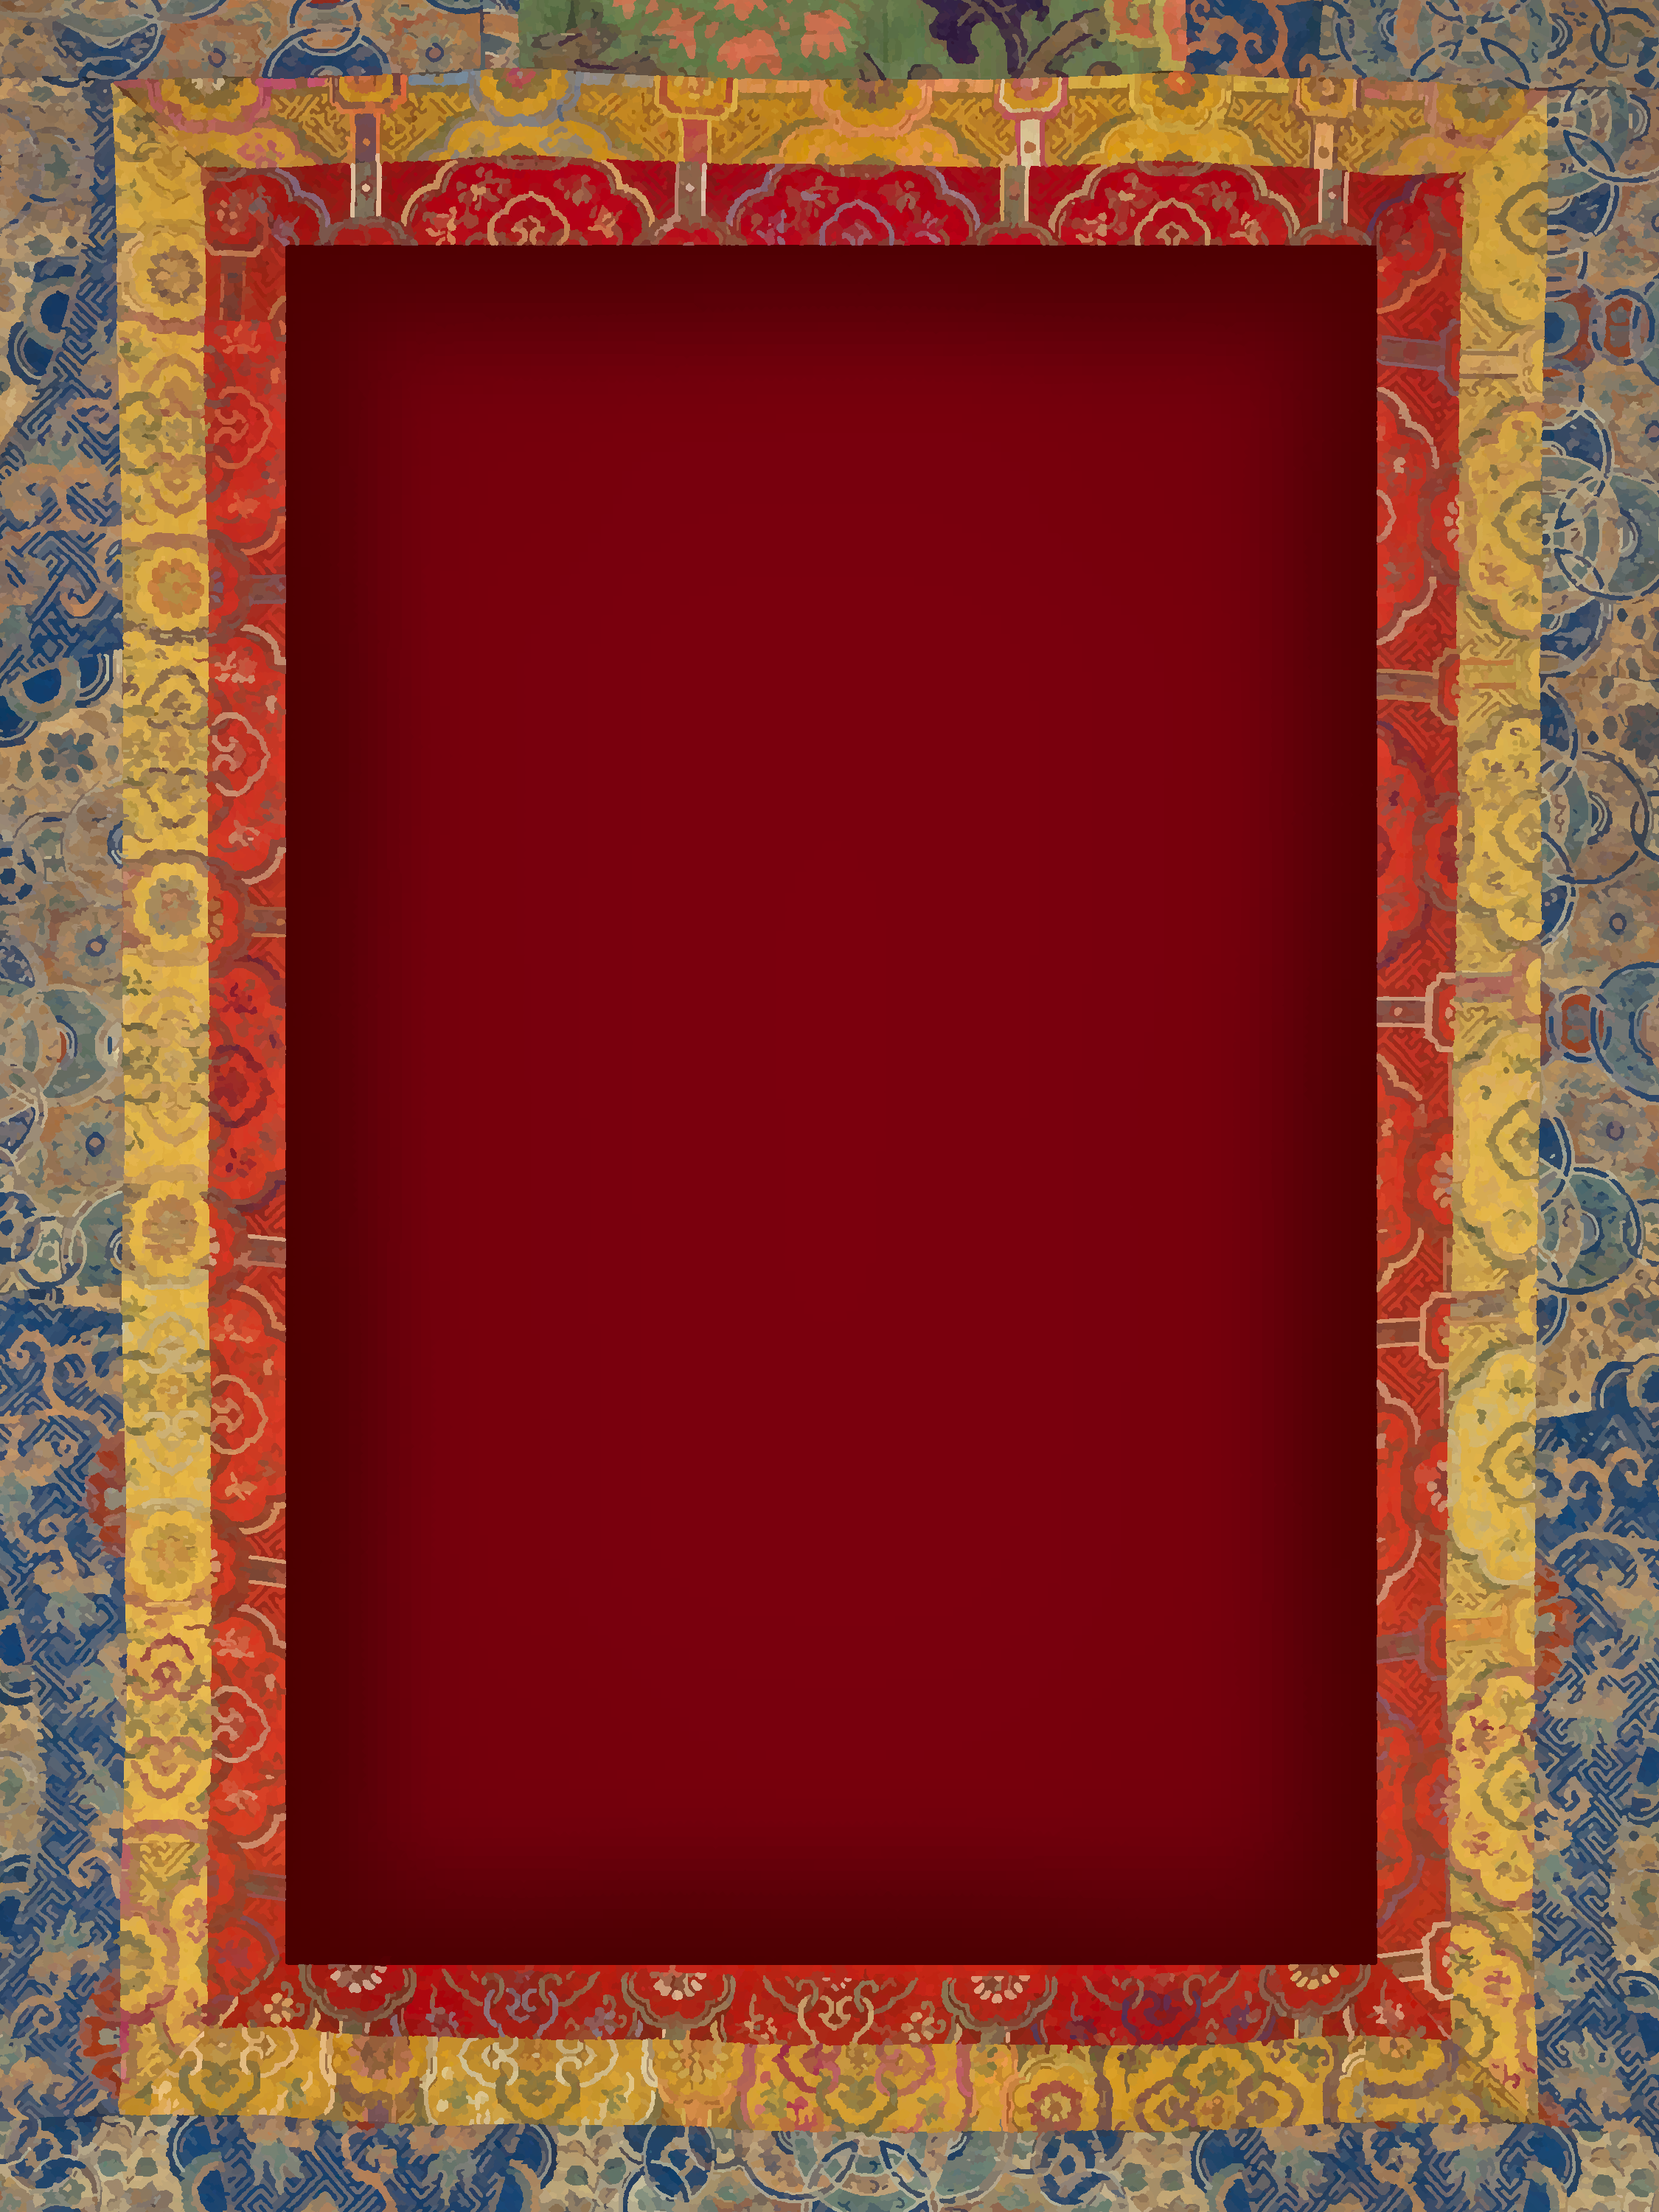
\includegraphics[width=\paperwidth,height=\paperheight]{tibet01.png}}

\renewcommand{\thefigure}{{\bfseries\color{customColor}\arabic{figure}}}

\renewcommand\thefootnote{{\bfseries\color{customColor}{\arabic{footnote}}}}
\let\oldfootnote\footnote
    \renewcommand{\footnote}[1]{\oldfootnote{{\bfseries\color{customColor}#1}}}
\bfseries    
\begin{titlepage} % Suppresses headers and footers on the title page
	\centering % Centre everything on the title page
	\scshape % Use small caps for all text on the title page

	%------------------------------------------------
	%	Title
	%------------------------------------------------
	
	\rule{\textwidth}{1.6pt}\vspace*{-\baselineskip}\vspace*{2pt} % Thick horizontal rule
	\rule{\textwidth}{0.4pt} % Thin horizontal rule
	
	\vspace{0.75\baselineskip} % Whitespace above the title
	
	{\LARGE Tibetan Paintings} % Title
	
	\vspace{0.75\baselineskip} % Whitespace below the title
	
	\rule{\textwidth}{0.4pt}\vspace*{-\baselineskip}\vspace{3.2pt} % Thin horizontal rule
	\rule{\textwidth}{1.6pt} % Thick horizontal rule
	
	\vspace{1\baselineskip} % Whitespace after the title block
	
	%------------------------------------------------
	%	Subtitle
	%------------------------------------------------
	
	{By \scshape\Large George de Roerich} % Subtitle or further description
	
	\vspace*{1\baselineskip} % Whitespace under the subtitle
	
	%------------------------------------------------
	%	Editor(s)
	%------------------------------------------------
	
	\vspace{1\baselineskip} % Whitespace before the editors

    %------------------------------------------------
	%	Cover photo
	%------------------------------------------------
	
	%\includegraphics[scale=1]{cover}
	
	%------------------------------------------------
	%	Publisher
	%------------------------------------------------
		
	\vspace*{\fill}% Whitespace under the publisher logo
	
	13, Rue Jacob. Paris (6\textsuperscript{e}), 1925 % Publication year
	
	{\small Librairie orientaliste, Paul Geuthner } % Publisher

	\vspace{1\baselineskip} % Whitespace under the publisher logo

    Internet Archive Online Edition  % Publication year
	
	{\small Attribution NonCommercial ShareAlike 4.0 International } % Publisher
\end{titlepage}
\setlength{\parskip}{1mm plus1mm minus1mm}
\setcounter{tocdepth}{3}
\setcounter{secnumdepth}{3}
\tableofcontents
\clearpage
\vspace*{\fill}
\begin{figure}[H]
\centering
\includegraphics[width=0.98\textwidth,keepaspectratio]{plates/plate-color.jpeg}
\caption*{Frontispiece. U\d{s}\d{n}\={\i}\d{s}a-Sit\={a}tapatr\={a}.}
\end{figure}
\vspace*{\fill}
\clearpage
\paragraph{}
\section*{Introduction}
\paragraph{}
It is only recently that the systematic study of Buddhist Art has been inaugurated. Thanks to scientific excavations and explorations carried out in India by the Indian Archaeological Survey, in Central Asia by a number of archaeological missions on behalf of different governments, and in China by the pioneer work of the eminent French sinologist, the late Edouard Chavannes, we possess a number of invaluable facts which enable us to reconstruct the vast domain of Buddhist Art. It is true that it is not yet possible to write a history of Buddhist Art in all its phases and different epochs. This huge work remains to be done, and we only can hope that future investigations in this field will facilitate the scholar's task. But if the complete history of Buddhist Art is still to be written, we can already affirm the unity of its evolution. No matter how different were the local influences, --- the types created by the joint effort of the Hellenistic genius and of the Hindu spirit, kindled by the doctrine of Buddha, maintained their originality throughout the centuries, --- from the caravan stations in the deserts of Chinese Turkistan to the island of Java. Indeed, it is a matter of great surprise that the sublime doctrine of Gautama, the Buddha, who established a legion of monks striving for a kind of ideal communism in this world, could have caused the rise of an art which powerfully attested itself throughout the vastnesses of Asia. Contemplating the serene simplicity of a Gandh\={a}ra Buddha, the delicate design of the Aja\d{n}\d{t}\={a} frescoes, the powerful and sometimes martial spirit of the Central-Asiatic pictorial compositions, and the religious fervor of the Wei art in the grottos of Yun-kang and Lung-men, --- we feel ourselves to be in the presence of a lofty altar of beauty erected by the united efforts of a host of Eastern and Western artists. No imaginary barrier stood or stands between these two great spheres of culture and civilization, and only petty racial prejudices have fostered the creation of a separating wall which haunts the imagination of a modern person. It should be remembered that the historic evolution of mankind never knew such barriers and that the message of culture proclaimed in one country is often acclaimed with equal enthusiasm in another country which may be located in a far distant part of our earthly globe. Such is the great attraction of ideas travelling along the routes that link nations together, not knowing what a barrier means. The future scholar will undoubtedly write a general history of the East, and he will also produce a history of Oriental art, which will demonstrate how great was the interchange between the various centers of culture in times gone by. When one thinks about the origins of Buddhist Art, one naturally turns towards India, the land where the Exalted One had preached his doctrine of universal salvation from the miseries of this world. But the scantness of reliable dates in the chronology of ancient India makes it very difficult to locate chronologically the outstanding creations of art produced on the soil of India. The existence of an art in India in pre-Buddhistic times can be left undoubted. Time and climate have destroyed whatever remained of the ancient architecture which used wood as its material, and it is only with great difficulties that we are able to sketch the history of the first plastic representations of Buddhist legends. Tentatives have already been made to discuss different tendencies in the art of the early periods, but all endeavors made by historical criticism have proved so far to be only theories, lacking in material foundations to become established facts. It seems certain that there existed a period of art strongly imbued with Greco-Persian influences. This art flourished under the Maurya dynasty (3\textsuperscript{rd} century \textsc{bce}). A fairly good example of this art is given by the capital of the A\'{s}oka column at S\={a}rn\={a}th, near Benares.

The next period is characterized by the funeral mounts or st\={u}pas of Bh\={a}rhut and S\={a}\~{n}ch\={\i}, which are solitary witnesses of a once flourishing artistic school. The differences in style and composition make it evident that various schools of art were active in the plains of India, and that the Buddhist artistic schools inherited much of the old local traditions, the nature of which it is impossible to ascertain at present. From the folk-lore tendencies of Bh\={a}rhut in Central India, erected about the middle of the second century \textsc{bce}, with its numerous reliefs representing scenes from the J\={a}takas, or stories of previous existences of the Founder of the Order, we pass to the group of funeral mounds of S\={a}\~{n}ch\={\i} (about the first century \textsc{bce}), rich in representations of miracles performed by the Exalted One during his preaching in the basin of the Ganges.\footnote{Sir J. Marshall, A Guide to Sanchi, Calcutta, 1918.}

The powerful influence exercised by the doctrine of Buddha on the minds of the people accounts for the efflorescence of an art dedicated to the glorification of the Master's earthly path, for, as the eminent French Indianist Professor Alfred Foucher has said\footnote{A. Foucher, The Beginnings of Buddhist Art, Paris, 1918, p. 35.}: ``I do not think that the imagination of any race has ever created a finer or vaster subject for a poem than this destiny of a single being in whom are shown all the aspects of life, in whom is concentrated all the experience of past ages, in one word, --- in whom the evolution of the entire race is reflected.''

The early Buddhist artists with singular fervor reproduced in plastic forms the various episodes of the early life of the Exalted One. The pious attention with which the Bharhut artists treated the work of representing the previous lives of the Buddha, made them inscribe below the reliefs the names of the J\={a}takas represented on them, thus giving to the modern scholar an unique opportunity of interpreting the early Buddhist images. The reliefs of S\={a}\~{n}ch\={\i}, although not inscribed with explanatory titles, are for the most part identified by Professor A. Grünwedel and Professor A. Foucher.\footnote{A. Foucher, ibid. pp. 61-110.} Most of the reliefs of this early Buddhist art can be satisfactorily explained with the help of the holy scriptures of Buddhism. Besides he numerous J\={a}taka scenes the early Buddhist reliefs represent the eight great miracles of the Buddha.\footnote{A. Foucher, ibid. pp. 147-184.} We easily recognize:

1. The scene of the Nativity (Skrt. J\={a}ti) in the park of Lumbin\={\i}, near Kapilavastu (the actual site has been commemorated by a pillar erected by A\'{s}oka, found near the present village of Rummindeî some 150 kls to the north of Benares).\footnote{E. J. Rapson, Cambridge History of India, Cambridge, 1922, p. 199.}

2. The perfect Illumination (Skrt. Abhisambodhana) on the site of the present Bodh-gay\={a}.

3. The first preaching (Skrt. Dharmacakrapravartana) at M\d{r}gadava, near Benares.

4. Death (Skrt. Parinirv\={a}\d{n}a), near the small town of Ku\'{s}inagara in the Nepal Terai.

These four sublime moments of Buddha's life, which were recommended for pilgrimage by the Exalted One himself, are supplemented by four others, which are the four principal occasions on which the Exalted One exercised his magical powers:

5. The Great Miracle (Skrt. Mah\={a}pr\={a}tih\={a}rya) at \'{S}r\={a}vast\={\i}.

6. The Descent from Heaven (Skrt. Dev\={a}vat\={a}ra) near S\={a}\.{n}k\={a}\'{s}ya.

7. The Offering of the Monkey near Vai\'{s}\={a}l\={\i}.

8. The Taming of the maddened Elephant at R\={a}jag\d{r}ha.

The Tibetan tradition knows another place of sanctity, which is left unknown in Indian tradition. It is the place where the future Buddha cut down his hair and pronounced his vow in the presence of Brahma and Indra. This place is characterized by a st\={u}pa, called in Tibetan ``the most holy st\={u}pa'' (mĕhod-rten rnam-dag), which is regularly seen on paintings picturing the prince Siddh\={a}rtha taking his monastic vow.\footnote{Cf. painting in the Collection Jacques Bacot in the Musée Guimet, described and edited by M. J. Hackin in his recent Guide-Catalogue du Musée Guimet, Paris, 1923, Pl. 19; a typical Tibetan mĕhod-rten or st\={u}pa is seen behind the figure of the Bodhisattva. In the Lalita-Vistara (ch. 15) we find the mention of a st\={u}pa called ``Chandakanivartana'' that has been erected on the place where Chandaka left the future Buddha. The text calls this place Anuvaineya, and adds that to reach this place one had to cross the territories of the \'{S}\={a}kyas, Kro\d{d}yas, Mallas, and Maineyas.}

It is almost impossible to say whether the early Buddhist art had produced an image of the Exalted One. A legend of the Divy\={a}vad\={a}na,\footnote{Burnouf, Intr. a l'hist. du Bouddhisme indien, p. 34.} which can be regarded as of a late period, tells us of the miraculous origin of the image of Buddha. The king Bimbis\={a}ra, of Magadha, having received rich presents from Rudr\={a}yana, king of Roruka, decided to send to the latter an image of the Exalted One. The artists, to whom the commission was given, found themselves unable to outline the divine face and figure of the Buddha. Seeing their difficulty, the Exalted One ordered a linen-cloth to be brought and on its surface projected his shadow, which was then designed and colored by the artists. We are involuntarily reminded of an almost analogical story concerning the miraculous origin of the image of Christ.

The artistic schools that decorated the funeral mounds of Bh\={a}rhut and S\={a}\~{n}ch\={\i} seem to avoid the human representation of the Exalted One. On the reliefs of Bh\={a}rhut and S\={a}\~{n}ch\={\i}, the Buddha is always represented by symbols, never in human form. Thus the Great Departure (Skrt. Mah\={a}bhini\d{s}krama\d{n}a) is always represented by a horse without a rider coming out of a city gate; the Great Preaching is symbolized by the Wheel of Law, and the Parinirv\={a}\d{n}a by a funeral mound or stǔpa.

As Professor Alfred Foucher has shown,\footnote{A. Foucher, L'Art Greco-Bouddhique du Gandh\={a}ra, Vol. 2\textsuperscript{nd}, fasc. 2, p. 744. Paris, 1923.} the two schools --- the one represented at S\={a}\~{n}ch\={\i}, and the other called Gandh\={a}ra school --- were almost contemporary. One, as we have just seen, used symbols to represent the person of the Teacher, as if denying the possibility of a representation in human form; the other succeeded in creating a human type of the Founder of the Order. It will be interesting to know whether there existed a correspondence between artistic schools and different sects of Buddhism. If such a correspondence could be discovered, the school represented at S\={a}\~{n}ch\={\i} should be regarded as the more orthodox of the two, corresponding to some Buddhist sects of Central India which zealously clung to the formula: ``The Buddha disappears, the Law remains,''\footnote{Mah\={a}parinibh\={a}na-sutta, 6, 1.} --- words which were spoken by the Exalted One himself at the time of his entering into Nirv\={a}\d{n}a.

The creation of a human type of Buddha has been, as we have just said, achieved by the Greco-Buddhist school that flourished in the ancient Gandh\={a}ra province in North-Western India towards the beginning of our era. This school had already established its character about the first century \textsc{bce}, and gained in eminence during the following centuries. About the third century \textsc{ce} its glory faded away and the subsequent centuries saw it in complete decadence.

This school was a typical product of its time, an outcome of the spread of artistic syncretism in the Hellenistic Orient of the last centuries before our era.

Since the memorable campaigns of Alexander the Great this craze for artistic and religious syncretism became general in the Near East, and has probably influenced North-Western India and Bactria, where Hellenistic dynasts established themselves after the dissolution of the great Macedonian Empire. The classical country of Hellenism was Egypt, where Greek emigrants persistently tried to establish a contact with the ancient lore of Egypt, and the Egyptians gradually admitted Greek conceptions into their religious system. The same general tendency was strongly pronounced in art, and the sometimes-clumsy type of Hellenistic artistic productions can be explained by the fact that the Hellenistic artist could not easily assimilate the great variety of different styles placed at his disposal. The Hellenistic tendencies of local dynasties in North-Western India and adjacent countries (Greek plays at Parthian courts), and the spread of Buddhist propaganda across the borders of India, resulted in the establishment of a local school of art. All the productions of this school bear evidence of its double origin: the form is undoubtedly Hellenistic, whereas the meaning can only be established with the help of Buddhist sacred texts.

At present we are in the possession of a monumental work by Professor Foucher on the art of Gandh\={a}ra, where its character, its artistic value, and its spread through the Buddhist world are masterfully described. We have dwelt on this school a little longer because of its important role in the history of Oriental art. Its creations were carried by sea and by land to the countries of the Far East, and established there the foundations of a brilliant efflorescence of artistic schools inspired by the doctrine and legend of Buddha.

The archaeological explorations which were carried out by a number of distinguished scholars along the two great caravan routes in Chinese Turkistan, have unearthed a huge amount of local artistic productions enabling thus to reconstruct the way by which the Gandh\={a}ra art had travelled before it reached the confines of China and powerfully influenced the religious art of the Wei period. The great drawback in the study of the Gandh\={a}ra art, and of the art of the early Buddhist period in general, is the complete absence of frescoes or other paintings. Time and climate have destroyed whatever remained of the old pictorial art. The walls of vih\={a}ras or monasteries and of rock-carved temples were undoubtedly decorated with frescoes, whose character it is impossible to ascertain. The Central-Asiatic pictorial art gives only a very imperfect idea of the character of the pictorial art of the ancient Gandh\={a}ra. Of the pictorial art belonging to the period preceding our era only one specimen exists: it is a fragmentary fresco in the Jog\={\i}m\={a}r\={a} cave of the R\={a}mgarh Hill in the distant Surguj\={a} State. According to Sir John Marshall the fresco was executed in the first century before our era. The original design of the fresco is spoiled by later restauration.\footnote{E. Rapson, The Cambridge History of India, ch. 26, pp. 642-43.} Let us hope that the recent archaeological explorations of Professor Foucher in Afghanistan, besides furnishing new proofs, will help us to fill this gap in our knowledge of Gandh\={a}ra art, and will give fresh material for a new chapter in the history of Indian pictorial art. The Gandh\={a}ra traditions left a lasting trace on the artistic schools of India, and the brilliant Gupta art owes much of its brilliancy to the achievements of Greco-Buddhist artists.

Tibetan art closely follows the ancient Indian traditions. Many iconographical types of the Buddhist pantheon in Tibet can be traced back to Gandh\={a}ra originals. Before discussing Tibetan pictorial art, a brief historical sketch of Tibet will be found useful.

Little is known about the history of the table-lands of Tibet\footnote{About the origin of the name ``Tibet,'' see Professor P. Pelliot, Quelques transcriptions chinoises de noms tibétains. T'oung-pao, 1915, pp. 18-20.} before the introduction of Buddhism in the first half of the seventh century \textsc{ce}. It seems that the country was ruled by a number of petty chieftains, who were in a state of continuous warfare against each other. According to Chinese Annals the first Tibetan kingdom was established about 607 \textsc{ce} by the king rNam-ri Sro\.{n}-btsan. His son was the famous ruler of Tibet, Sro\.{n}-btsan sgam-po, who introduced Buddhism into the land and whom the tradition honors with the title of Čhos-rgyal, or Dharmar\={a}ja. This king established his capital in Lha-Idan or Lha-sa in Central Tibet (dbUs), and laid the foundations of a state organization. His victorious conquests carried him to the confines of China and his armies even sacked the western Ssǔ-ch'uan province. About 640 \textsc{ce} he concluded a peace treaty with the T'ang Emperor T'ai-tsung, by which his supremacy in the region of Kuku-nor was recognized by China. And such was the military strength of the Tibetan king that he even obtained in marriage a Chinese Imperial princess (kung-chu). Sro\d{n}-btsan sgam-po concluded another matrimonial alliance with Nepal by marrying the daughter of the Nepalese king Am\'{s}uvarman. These two royal princesses were fervent Buddhists, and tradition says that the Chinese princess brought to Tibet a famous statue of Buddha, while the Nepalese princess brought an image of the Dhy\={a}ni-Buddha Ak\d{s}obhya. Both statues are now preserved in the Jo-khang in Lhasa. It is even said that the king married the two princesses in order to obtain the two famous statues.

It is through the influence of these two princesses that the king accepted Buddhism and fostered its spread in his kingdom. The grateful Buddhist Church of Tibet regards the two foreign princesses as incarnations of the divine T\={a}r\={a} under her green and white aspects (Tib. SGrol-lja\.{n}, and sGrol-dkar). Sro\.{n}-btsan sgam-po sent to India a number of gifted young men, among whom was the famous Thon-mi Sambhota, the inventor of the Tibetan alphabet and the author of the first Tibetan grammatical work in \'{s}lokas.

After the death of king Sro\.{n}-btsan sgam-po little progress was made by the new religion, and only with the advent of king Khri-sro\.{n} lde (lde'u)-btsan (755-797 \textsc{ce}), the spread of Buddhism gained a new impulse. This king, besides being a conqueror, was a great patron of the new religion, and invited to Tibet the great \'{S}antarak\d{s}ita of N\={a}landa and the Buddhist monk Kamala\'{s}\={\i}la. This last one became famous because of his religious controversy with the Ho-\'{s}ang Mah\={a}y\={a}na, a Chinese monk regarded in China as an incarnation of Maitreya, the future Buddha.

The Buddhism that reached Tibet was already strongly imbued with \'{s}ivaïtic influences and other beliefs in magical practices, which were regarded with such an abhorrence by early Buddhists. Professor de la Vallée Poussin in the learned introduction to his valuable ``Études et Matériaux''\footnote{Prof. de la Vallée Poussin, Bouddhisme, Études et Matériaux, p. 33 and 37.} has already indicated the existence of a scientific Buddhism, a Buddhism of a comparatively small number of learned doctors, and of a popular Buddhism which introduced into the system a number of popular beliefs. The pandit \'{S}\={a}ntarak\d{s}ita advised the king to invite from India the great tantric teacher Padmasambhava of O\d{d}\d{d}iy\={a}na.

Padmasambhava was an adopted son of king Indrabh\={u}ti of O\d{d}\d{d}iy\={a}na. In the Padma Tha\.{n}-yig,\footnote{Padma Tha\.{n}-yig; portions of the work have been translated by M. Toussaint. See bibliography.} a bulky work relating the legendary life of Padmasambhava, it is told how the future teacher was found by the king and his minister sitting on a lotus flower in the middle of a lake called Vimalaprabh\={a}, how he married and left the palace, how he led an austere life in a cemetery called the ``Cool grove'' (Tib. bSil-ba tshal-gyi dur-khrod), and how he became known by his many miracles. The second part of the work contains an account of his mission to the ``Land of the Snows.''

The great Guru, or Mah\={a}c\={a}rya, on his coming to Tibet, had a difficult task before him. He met with a violent opposition on the part of the local religion, probably a kind of Bon, and of many people of influence at the royal court. He overcame all the barriers put before him and accepted a number of local cults into his system. This he did in order to calm his opponents. His followers in Tibet are known under the name of rÑi\.{n}-ma-pa, and are distinguished by their red caps. The rÑni\.{n}-ma sect is essentially a Tantric school and is still influential in the Himalayan Border States. The sect regards the Bodhisattva Samantabhadra as a primordial Buddha, and a special cult is dedicated to him. Besides this Bodhisattva, the cults of the Yi-dam rDo-rje phur-pa and other mGon-po, or ``protectors,'' are strongly recommended by the founder. The system is characterized by a great number of hidden scriptures or gTer-ma discovered from time to time by lamas, and said to contain mystic doctrines. The titles of the hidden books are sometimes given in some unknown language, whose meaning it is impossible to ascertain at present.\footnote{We believe these languages to be artificial languages.} The chief occupation of the followers of this sect is Magic and other ceremonies prescribed by various Tantras. Padmasambhava also assisted king Khri-sro\.{n} lde-btsan in the building of the monastery of bSam-yas-gling, the treasury of the present Lhasa Government. He also began the work of translating the Buddhist books into Tibetan, assisted by the Lo-tsa-ba Pagur Vairocana. The stay of Padmasambhava in Tibet was not a very long one and he soon returned to India.

After the death of king Khri-sro\.{n} lde-btsan Buddhism continued to spread in Tibet. A number of Hindu doctors were invited to Tibet to continue the preaching and the translation of Buddhist texts. A heavy blow to the new doctrine, was delivered by gLa\.{n}-dar-ma, who was proclaimed king about 838 \textsc{ce}, after the murder of his brother, the pious and weak Khri Ral-pa-čan. The short reign of gLa\.{n}-dar-ma was full of violent outbreaks against the doctrine of Buddha. The Indian pandits were driven away from Tibet, books were destroyed, and temples devastated. Only a few lamas succeeded in hiding the scriptures from destruction. Fortunately for Buddhism, the king was murdered by a lama-hermit, dPal-rdo-rje, who approached the king in the disguise of a Bon magician. The memory of this event is still living among the Tibetans of today, and one of the lama religious dances, namely the Black-hat dance, purports to represent this event.

In the 9\textsuperscript{th} century \textsc{ce} we see the Tibetans at the height of their military strength, extending their occupation even into Chinese Turkestan and taking possession of the important oasis of Tun-huang in the western Kansu province, where Sir Aurel Stein and the eminent French sinologist Professor Paul Pelliot made their brilliant discoveries. But the military power of Tibet did not last more than two centuries. With the spreading of Buddhism the martial spirit of the warlike nomads gradually faded away. From now on religious interests occupy the minds of the people and of their sovereigns. Among the Tibetan kings of this period many accepted monkhood. In the 11th century \textsc{ce} the lama-king Byan-čhub-'od invited the famous Indian pandit At\={\i}\'{s}a, otherwise Dip\={a}\.{n}kara\'{s}r\={\i}j\~{n}ana, of the great convent of Vikrama\'{s}\={\i}la.

This outstanding personality in the history of Buddhism in Tibet brought with him the K\={a}lacakra system (Tib. Dus-kyi 'khor-lo), and preached against the magic rites and Tantric cults of the rÑi\.{n}-ma sect. The school of purer Buddhism founded by At\={\i}\'{s}a is known under the name of bKa-gdams-pa, and lays stress on meditation and a severe discipline in the monasteries. Under his guidance a number of texts belonging to the Vinaya (Tib. 'Dul-ba) and the S\={u}tras (Tib. mdo) were translated into Tibetan. About 1050 \textsc{ce} a religious council took place in Central Tibet under the presidency of At\={\i}\'{s}a and proclaimed the reestablishment of the doctrine of Buddha in Tibet. At\={\i}\'{s}a was the author of many well-known works and can be regarded as the true predecessor of rGyal-ba Tso\.{n}-kha-pa, the founder of the Yellow-cap sect. At\={\i}\'{s}a died in 1058 \textsc{ce}.

One of his pupils, the great Tibetan historian 'Brom-ston (born about 1002 \textsc{ce}), systematized the rules of the bKa-gdams-pa sect and founded the monastery of Rva-sgreng (pron. R\={a}-deng) to the North-East of Lhasa on the caravan route to the region of Kuku-nor.

The period from the 11 century to the 13 century \textsc{ce} witnessed a gradual growth of Buddhism on the Tibetan tableland. The number of monasteries steadily increased and a greater percentage of the population accepted monkhood, seeking salvation. A number of monasteries gained great power and their abbots often took an active part in the political feuds of the country. Great was the influence of the Saskya Monastery, which was founded about 1071 \textsc{ce} by 'Khon-dkon-měhog rgyal-po, and whose abbots played such an important rôle at the Court of the Mongol conquerors.

The Mongol tribes, which, since the 8\textsuperscript{th} century \textsc{ce}, were already in contact with the Buddhist Uighur tribes, accepted Buddhism in the 13th century \textsc{ce}. This was a period of an exceptional prosperity of the doctrine, under the mighty patronage of the Mongol khans. One of the greatest abbots of Saskya, generally known under the name of Saskya pan-čhen or pa\d{n}\d{d}ita, was invited by Godan Khan, son of Ogödäi, to visit his residence in Kan-su. The Saskya pontiff, besides spreading the doctrine of \'{S}\={a}kyamuni, is said to have invented for the Mongols an alphabet based on the Uighur script.\footnote{G. Schulemann, Die Geschichte der Dalailamas, p. 51.} His work was continued by his nephew and successor, the lama 'Phags-pa  bLo-gros rgyal-mtshan (Skrt. Matidhvaja \'{s}r\={\i}-bhadra, 1239 or 1240-1280 or 1281 \textsc{ce}), who invented a new script based on the Tibetan alphabet and offering a more correct transcription of Mongolian.\footnote{Prof. Pelliot, Course delivered at the Collège de France, 1922-1923; B. Laufer, Skizze der Mongolischen Litteratur, p. 185.} Khubilai Khan, who transferred the capital from Karakorum first to Shang-tu in 1260 and finally to Peking (Ta-tu) in 1264 \textsc{ce}, conferred upon the lama 'Phags-pa the title of ``Imperial Preceptor'' (Ti-shih). With the fall of the Yüan dynasty in 1368 \textsc{ce}, Buddhism experienced a severe blow and regained its influence only about the end of the 16\textsuperscript{th} century.

It was in 1357 \textsc{ce} that was born the great Tibetan Reformer rGyal-ba Tso\.{n}-kha-pa,\footnote{All students of Tibetan history will do well to study the illuminating article of Prof. Pelliot, Le cycle sexagénaire dans la chronologie tibétaine (J. As. 1913), before using the works published in European languages on Tibetan history; p. 667, n. 3.\\\hspace*{5mm}We hope to bring out in the nearest future a volume on the Life of Tso\.{n}-kha-pa, being a translation of the biographical portions of the rGyal-ba Tso\.{n}-kha-pa'i bka-'bum.} who succeeded in establishing the religious supremacy of his sect in Tibet. His birthplace is situated in the Amdo region. To commemorate this place, the great convent of sKu-'bum was built. Space forbids us to relate in detail the legend of Tso\.{n}-kha-pa, his solitary life in the mountains, his studies in the famous monasteries of Tibet, and his activity as preacher at Lhasa. From the days of his early youth he was strongly bent on religion, and very early he entered the order under the monastic name of rGyal-ba bLo-bzan grags-pa (Skrt. Sumatik\={\i}rti).

The advent of Tso\.{n}-kha-pa marks the return to a purer form of Buddhism already preached by At\={\i}\'{s}a, his glorious predecessor in the field. The austere monk made celibacy obligatory for all monks and forbade the \'{s}akti rites of the old Tantric schools.\footnote{G. Schulemann, ibid., p. 82, says that rgyal-ba Tso\.{n}-kra-pa allowed in the monasteries the study of dKar-rtsis (Weisse Wissenschaften), and forbade the practice of Nag-rtsis (Schwarze Magie).\\\hspace*{5mm}DKar-rtsis does not mean here ``white magic,'' and should be read as sKar-rtsis, which usually denotes astronomy and astrology according to Indian tradition. Nag-rtsis is a contracted form for rGya-nag-gi skar-rtsis, or ``Chinese Astronomy.'' A number of Tibetan astronomical and astrological books have been translated from Chinese.} He laid great stress on the morals and discipline of the monks and called his school dGe-ldan-pa or dGe-lugs-pa, ``the virtuous.'' The first great monastery of this school, called dGa-ldan, was erected about 1409 \textsc{ce}\footnote{Huth, Geschichte des Buddhismus in der Mongolei, vol. 2, p. 183.} in the neighborhood of Lhasa.

Tso\.{n}-kha-pa left a number of remarkable works on Buddhist metaphysics, of which the best known is the Lam-rim čhen-po or Byan-čhub lam-gyi rim-pa, ``the Steps of the Bodhi-path.'' This work is thoroughly studied in the theological schools at the great monasteries of Lhasa, such as Sera or 'Bras-spu\.{n} (pron. De-pung); and some of the convents of Mongolia, such as Porhantu and Tala,\footnote{Laufer, ibid., p. 223; Huth, ibid., p. 375.} have special Lam-rim seminaries. The foundations of the present Church organization in Tibet were laid down by Tso\.{n}-kha-pa.

rGyal-ba Tso\.{n}-kha-pa is said to have had as his spiritual guide the Bodhisattva Ma\~{n}ju\'{s}r\={\i}, who appeared to him in the solitudes of the Amdo mountains. He is believed to have sometimes obtained his inspiration from Maitreya himself, and in this connection lies, perhaps, the explanation of the extraordinary spell exercised by the teachings of the great Reformer on the mind and soul of the Lamaistic monkhood. The work of Tso\.{n}-kha-pa was carried on by his two principal disciples: mKhas-grub-rje (full name mKhas-grub dGe-legs dpal-bza\.{n}, 1385-1439 \textsc{ce}), and rGyal-tshab-rje. mKhas-grub-rje was appointed abbot of the dGa-ldan Monastery. Another pupil of Tso\.{n}-kha-pa, Byams-čhen čhos-rje, also called \'{S}\={a}kya Ye-\'{s}es, on the invitation of the Ming Emperor Yung-lo, was dispatched by Tso\.{n}-kha-pa to China, where he preached the K\={a}lacakra doctrine.

On his return to Tibet he founded the monastery of Sera, near Lhasa (1419 \textsc{ce}). Tso\.{n}-kha-pa died in 1419 \textsc{ce} in the dGa-ldan Monastery. In the following collection of paintings there are seven modern paintings representing the Great Reformer in various attitudes; we shall describe them in the course of our study. The Ming Emperors were in general favorably inclined towards the Lamaistic form of Buddhism, as they were eager to maintain their political protectorate over Tibet.

The first rGyal-ba or ecclesiastic ruler of Lhasa was the nephew of Tso\.{n}-kha-pa, Mah\={a}pa\d{n}\d{d}ita dGe-'dun grub-pa. In the year 1445 he erected the great Monastery of bKra-\'{s}is lhun-po (pron. Tashi-lhunpo) at Shigatse, whose first bKra-\'{s}is lama, according to tradition, was mKhas-grub-rje.

In 1576 \textsc{ce}\footnote{Huth, ibid., p. 215.} the famous Altan Khan, the qavan of the Tümäd, conferred upon the Grand Lama of Lhasa, mKhas-grub bSod-nams rgya-mtsho dpal-bza\.{n}-po (the 3\textsuperscript{rd} rGyal-ba or rGyal-dba\.{n}), the title of Dalaï (Tib. rGya-mtsho-ocean) Lama Vajradhara, and recognized the religious supremacy of the Yellow faith. China continued to exercise her political domination, and in 1793 the Emperor Chien-lung of the Manchu dynasty promulgated an imperial edict correcting the system of reincarnation by which new Dalaï-Lamas were nominated and ordered the investiture of candidates by the Chinese Government.

It would require too much space to record one by one all the reigns of the thirteen Dalaï-Lamas of Tibet. The recent history of Tibet is full of events, and it is difficult at present to foresee the outcome of many of them.

After this brief sketch of Tibetan history, it will be easier for us to discover the many influences that penetrated into the ``Land of the Snows'' and enriched the vast pantheon of Tibetan Buddhism. The high mountain ranges which on all sides surround the tablelands of Tibet did not stop the penetration of foreign influences. In the early days of Tibetan history the trade routes from Tibet into the plains of India passed across western Tibet. By these routes, often not more than narrow mountain trails, Indian artistic traditions reached Tibet. The Buddhist missionaries who entered the country in the 7\textsuperscript{th} century brought with them the first sacred images. These images probably served to illustrate their preaching and consisted of the most important representations of the Buddhist iconography, namely: images of the Exalted One himself, of the principal Bodhisattvas, and images representing scenes from the legendary life of the Master. It is a significant fact that precisely in these images we see the strongest Indian influence. Many types of the Buddhist iconography of Tibet can be traced back to the Gandh\={a}ra School in North-Western India, but one should not forget that it was a Gandh\={a}ra art of the period of decadence that served as model to Tibetan artists.

From an early date Tibet came into close contact with its Southern neighbor Nepal. The Nepalese pictorial art steadily influenced the Tibetan conceptions of beauty. It was through this art that the Tibetan artists acquainted themselves with the traditions of the Aja\d{n}\d{t}\={a} frescoes. In the 13th and 14\textsuperscript{th} centuries this influence of Nepalese art reached its height and even penetrated to the Imperial Court of China. Nepalese artists were highly reputed for their skill and were frequently summoned to the great lamasaries of Tibet. In the Yüanshih, the history of the Yüan dynasty (ch. 203), there is a short biography of one of such artists called A-ni-ko (Anigo), born in 1243.\footnote{For all this information concerning this Nepalese artist, I am indebted to the course delivered by Prof. Pelliot at the College de France in 1922-23; the Edition revised by the commissaries of Ch'ein-lung has the form A-erh-ni-ko. In the history of the 84 mah\={a}siddhas published by Prof. Grünwedel mention is made of a person called Anigo. Prof. Sylvain Lévi, Le Nep\={a}l, vol. 3, p. 185-189.} This skillful molder went to Tibet in company with several fellow-artists from Nepal to execute some work in Tibet, and was subsequently invited to the Court at Peking, where he was entrusted with important restauration work. A number of statues in the Buddhist and Taoist temples of China are said to be the work of this celebrated master.

It is a well-known fact that sculpture is always more conservative, and it is among Tibetan bronzes that we still find specimens strongly imbued with an Indo-Nepalese influence.

Besides this Indo-Nepalese influence from the south, other influences were at work in Tibet. Tibet was always in active relation with the region of Khotan (Tib. Li-yul) in Chinese Turkestan, and there can be no doubt that the Khotanese local artistic productions found their way into Tibet and had an influence on its art. These artistic productions were of a very composite nature, still bearing traces of an Indian past. They belong to this complex world that has been created in Central Asia through a contact of a number of nations. The types of the sixteen arhats, of different religious protectors with their warlike following of devas and yak\d{s}as, all clad in armor, can be considered as importations from the North.

About the tenth century \textsc{ce}, when Mohammedanism spread itself over Central Asia bringing destruction of the ancient Buddhist communities along the great caravan routes, many of the monks of Turkestan found refuge in the monasteries of Tibet and brought with them traditions of their respective localities.\footnote{A. Foucher, L'art gréco-bouddhique du Gandh\={a}ra, vol. 2, fasc. 2, p. 672.} Chinese art never strongly influenced the art of Tibet: on the contrary, some iconographical manuals edited during the Ming period clearly exhibit a predominant Nepalo-Tibetan influence. During the 17-18\textsuperscript{th} centuries the Chinese influence became evident in design and ornamentation. The painting, representing the mGon-po phyag-drug in this collection, can be regarded as an example of this semi-Tibetan art. Notice that the design of this period is more free in its character and in the abundance of rich floral motives in the ornamentation.

Our present knowledge of Tibetan pictorial art is not sufficient to enable us to discuss various schools of art. But, notwithstanding many discrepancies in our knowledge of the subject, we are able to distinguish at least two areas or spheres of artistic activity --- the South-Western and the North-Eastern; the first has as its center the town of Shigatse, in whose neighborhood is situated sNar-tha\.{n}, the biggest printing establishment in the country; the school of Shigatse is tributary to the Indo-Nepalese art, and paintings produced by artist monks of the great convent of Tashi-lhunpo follow the traditions inherited from India.

The North-Eastern school has as its center the province of Derge. This school originated in the neighborhood of the great caravan route from the plains of Mongolia and Western China into Tibet, and is, therefore, strongly imbued with outside influences coming from the North.

Although the foundations are formed by the same Indo-Nepalese art, the later additions point towards Mongolia and China. In paintings coming from Derge (it is only very seldom that one can tell the origin of a painting) we see people dressed in heavy overcoats, fur caps, and boots, and wearing ornaments that could belong to a witch doctor of Eastern Siberia. Some of the representations bear a striking resemblance with the figures of donors of Turko-Mongolian nationality, represented on some frescoes of Tun-huang. The Bodhisattva type met on the Derge paintings reminds us of the Bodhisattva images of the T'ang epoch, attired in a royal fashion that resembles more the costume of a Central Asian Bodhisattva than the princely attire of an Indo-Nepalese Bodhisattva. Such are the two big artistic schools of Tibet. It is impossible to say how far back we can trace their existence, for Tibetan art is entirely anonymous and the complete absence of dates makes it almost impossible to reconstruct chronologically the outstanding events of Tibetan artistic history.

Besides the two big schools, there are a number of local schools, such as the Lhasa school, the Gyangtse school, and the school in the Khams province in Eastern Tibet. In the ancient period the unity of style was greater. The differences between the various local schools became more accentuated in modern times; the peculiarities of styles can be discerned only by an expert eye. Usually each one of the Buddhist sects of Tibet has something of its own in the style of paintings produced by artists belonging to the sect.

We shall note the origin of paintings and the peculiarities of styles of various schools, if discernable, in the process of our description.

Let us now pay a visit to the studio of a Tibetan artist-painter and watch the process of his work. But before starting with our description, we shall have to make a number of preliminary remarks of a general character. It is surprising that religious art in all countries, from the high tablelands of Tibet to the mediaeval workshops of Italian masters of the early Renaissance, have created analogical methods, and, what is still more surprising, a similar atmosphere, of work. For a better understanding and appreciation of Tibetan religious paintings (for art in Tibet is entirely religious), a knowledge of conditions in which the painter's work is carried out is essential. There is in Tibet no big school where future artists receive their training, but, like in the Italy of the Renaissance period, or in old Russia, each master has a number of pupils who live with him and help him in his work. Such was the order of things in ancient times, and a similar custom continues to exist in the Tibet of the present day. There is always a great number of painters in big centers of religious life, such as Tashi-lhunpo, or one of the great Yellow-cap monasteries near Lhasa, where big decorative work is always going on. The Dalaï Lama of Lhasa and the Tashi-Lama have always a staff of artists in their service. It is only seldom that a Tibetan artist stays a long time in one place. Usually he is travelling from one place to another, working in houses of rich laymen, or executing mural decorations in some of the big monasteries. In his wanderings he visits many outlying places of Tibet, makes himself acquainted with local styles, and in his turn introduces into the local art something of his own style. Thus the wandering character of the life of a Tibetan artist may be regarded as one of the causes of the similarity of art objects produced in different provinces of Tibet.

We have already discussed the possible foreign currents that exercised their influences on Tibetan art in the various epochs. We have even made the attempt to arrange chronologically such influences on Tibetan art in the various epochs, being fully aware of the difficulties presented by the subject. At such places as sNar-tha\.{n} near Shigatse, or in one of the big printing houses of Derge, iconographical collections of images have been printed in black and red ink, giving the outlines, but not the coloring. Such printed outlines are widely used by artists in Tibet, and are known under the technical name of tshags-par, which means literally ``dotted impression.'' We call this kind of printed outline --- ``transfer.'' The outlines printed at Derge are far better in execution, and their lines are sharper because printing at Derge is done from metal plates.

This kind of transfer is applied to the surface on which the painting will be made, then a needle is taken, with which the artist goes over the outline. The dotted lines thus produced on the surface of the paintings are then delineated with red or black ink. It is curious that exactly the same method is in use among Russian ikon painters, and ``Corona Mundi'' is fortunate to possess a collection of such ``transfers'' used among the ikon painters in Russia. The wide application of the transfer method made it almost impossible to find in Tibet a clever draftsman, who could sketch an image by free-hand drawing. Only very seldom can such an experienced draftsman be found, and in such cases there is always the danger that the image produced by him will not be canonical in all its detail, for it is almost impossible for one man to remember all the innumerable details of Tibetan iconography. The existence of such ``transfer'' work has created a rigid style of design, and we look in vain in Tibetan pictorial art for the masterful stroke of the brush of a Chinese artist. We have already pointed out that the interest of Tibetan paintings lies in their rich coloration, and their decorative possibilities can hardly be overestimated.

The most characteristic production of Tibetan pictorial art is the so-called tha\.{n}-ka, a word which is commonly interpreted as ``banner.'' Such tha\.{n}-ka are in multitudes found in temples and private houses. They are always carried in religious processions and often serve to illustrate a religious sermon. Wandering lamas are sometimes found in the possession of a good assortment of such paintings, which serve them in their preaching, --- for art in Tibet, and in other lamaïstic countries, was and is a powerful ally of the propagation of Buddha's doctrine.

In the ancient language, instead of the word tha\.{n}-kha and its two corresponding honorific expressions šal-tha\.{n} and \d{s}ku-tha\.{n}, other words, like ri-mo ``picture,'' and \d{s}ku-br\.{n}en, ``figure, image,'' were in use. 

Besides painted banners, a Tibetan painter executes mural paintings, sometimes on a very large scale and of an extremely complex composition. We remember having seen a number of mural decorations executed by modern Tibetan artists in the monasteries of Sikhim, and are glad to state that the old tradition is still alive. The design of such mural decorations often shows an experienced hand, and their color scheme is often very striking. Often the artist in Tibet is called to decorate pieces of furniture both in temples and private houses, temple altars, and the ceremonial trumpets of the Lamaïst divine service. Masks used in religious dances are also decorated by artists; and the outside walls of houses are sometimes found painted in bright colors. For the last kind of work the artist uses a special ornamentation, derived from a purely religious ornamentation; holy symbols, the svastika, the Wheel of the Law, and rich floral designs predominate in such decorative motive.

After this very brief sketch, let us make a closer study of the process itself by which a painting is made in Tibet. We are sure that the reader will excuse us for dwelling a little longer on this particular question, but we are certain that a visit to the studio of a Tibetan artist will greatly help our purpose.

The artist is usually a lama, more or less versed in sacred scriptures. He accompanies his work by a continuous reciting of prayers. Prescriptions for artists, found in the Känjür, tell us that he must be a saintly man of good behavior, learned in scriptures, and reserved in his manners. The saintly image can only be painted in a clean place and, therefore, the studio of an artist is always comparatively clean. The artist himself is usually found sitting on the ground, holding the painting on his knees. Round him are seated his disciples who prepare colors and attend to the various needs of their master. Sometimes an advanced student helps his master in the work by coloring the outlines of figures drawn by the master.

In Tibet, paintings are usually painted on silk or on other thin cloth, which is stretched on a frame. After the silk has been stretched, it is thickly covered with a mixture of glue and chalk, which is then well polished with the smooth surface of a conch. When this is finished, the outlines of the figures are drawn with red or black ink. Mongolian artists often use skin instead of silk.

The work is carried on very slowly, for even minute details of the ornamentation must be attended to before coloration is started. To make a mistake in the measurements of a body given in the iconographical manuals is considered to be a great sin. Sometimes another lama is present, whose duty it is to read aloud prayers while the artist is at work. And so intense is the religious atmosphere which surrounds the creation of a painting, that the face of a Buddha or Bodhisattva is preferably drawn on certain auspicious dates. Throughout Tibet the 15\textsuperscript{th} and 30\textsuperscript{th} days of each month are considered to be sacred, and the artist usually draws the features of the faces on the 15\textsuperscript{th} day of the month, and colors them on the 30\textsuperscript{th} day.

After the design is finished, the artist begins the coloration, whose decorative tendencies we have already stated. Those who know the methods applied by Russian ikon painters will not fail to recognize the great similarity between the two methods. Indeed, it seems that the Russian ikon art and the Tibetan pictorial art derive their methods of work from a common source.

In Tibet an experienced draftsman is seldom a good painter and, likewise, a fine painter is seldom a clever draftsman. Usually the draftsman makes the design and the painter puts the colors on it. Such a distribution of work is also found among the Russian ikon painters, and, therefore, they always go about in small companies. As in the case of the Tibetan artist, the Russian ikon painter before starting the painting, covers the wooden board with a similar mixture of chalk and glue (the mixture is technically called ``levkas''), which is afterwards polished. Similar is also the process of painting itself: first the design, elaborate in every detail, and then the colors. In both cases no sketch work is done, everything being drawn according to firmly established canonical rules: first the principal figures, then the surroundings, sky, hills, trees, etc.

A comparative study can be pushed much further, for even in the composition itself we find common elements. Thus we often see on Tibetan paintings the principal figure enthroned on an island (this being usually the case when Buddha or Bodhisattva is represented). Similar images are frequently found on Russian ikons, the island being a conspicuous element in the landscape. The landscapes themselves, especially the way of representing mountains, rocks, and clouds, are similar in both arts. It is difficult at present to describe Tibetan artistic methods in detail, for each painter zealously guards his own secret of work. There exist in Tibet a number of artistic manuals in which many a detail could be of great interest for a comparative study. Among these manuals, one of the chief ones is the so-called ``Vai\d{d}\={u}rya ser-po''\footnote{Mr. J. van Manen, in his valuable ``Contribution to the Bibliography of Tibet'' (J. A. S. B., vol. 18, Nr. 8, 1922) mentions on p. 511 a Vai\d{d}\={u}rya Ser-po, which seems to be a history of the Yellow-hat sect. It will be interesting to know whether the iconographical manual Vai\d{d}\={u}rya Ser-po forms a part of the historical work quoted by Mr. van Manen, or is a separate work. The Bai-ser (yellow vai\d{d}\={u}rya) mentioned by Mr. van Manen --- is a historical work.}; the fifth rGyal-ba of Tibet is said to have composed a number of treatises on art.

We feel confident that if these texts could be translated and commented on, further striking analogies between Russian ikon art and Tibetan pictorial art would be discovered, for Russian ikon art preserves many artistic traditions of the Orient. Russian ikon art is generally said to have originated from Byzantium. This is historically true, but one should not forget that Byzantine art, especially in its late periods, was essentially oriental and that, through Byzantium, the Indio-Persian influences penetrated into Mediaeval Russia. Then came the Mongol invasion which lasted for several decades, and violently put Russia face to face with the whole of the Middle East. Besides destructions and war, the Mongols brought with them the color-schemes of Oriental art and introduced into Russian religious art new motives, whose eastern origin cannot be denied.

Those who have collected Tibetan paintings know how difficult it is to obtain good specimens. A Tibetan will never part with a tha\.{n}-ka, especially if it is consecrated by some high lama and has the imprint of the lama's hand on its reverse side. The painting of this collection representing the Yi-dam Vajrak\={\i}la has such a handprint on its back. To induce a Tibetan to sell a painting to non-buddhists or, as they are called in Tibetan language, ``outsiders'' (Tib. phyi-rol-pa, pron. či-rol-pa), is almost a hopeless task. Most of the paintings found in European public and private collections have been thrown on the market as the result of recent wars and upheavals in Tibet, which brought the destruction of several lamaseries and the ruin of rich families, which were in possession of numerous religious paintings.

The time has not yet come to write a history of Tibetan art. Such a study necessitates a detailed description of all the collections of Tibetan art preserved in European Museums. Many good paintings are undoubtedly in the possession of private persons, but, unfortunately, we do not possess a list of such private collectors. Museum collections themselves hardly possess detailed catalogues and well executed photographs which could serve our purpose. The only collections of Tibetan paintings and bronzes which were studied and described in detail are the collections of Prince Ukhtomsky in Petrograd, Russia, on which was based the ``Mythologie des Buddhismus in Tibet und der Mongolei'' by Professor Grünwedel, and the rich collection of paintings brought back from Tibet by Mr. Jacques Bacot and now preserved in the Musée Guimet in Paris. This last collection has been thoroughly studied and scientifically described by Mr. J. Hackin, the learned curator of the Museum. Mr. Hackin deserves our grateful thanks for publishing a ``Guide-catalogue du Musée Guimet,'' in which the Buddhist collections of the Museum are described. Let us hope that other Museums will follow this enlightened example and will furnish us with detailed catalogues of their Buddhist collections.

The Ethnographical Museum of Berlin, the Field Natural History Museum in Chicago, the British Museum, the Ethnographical Museum of the Russian Academy of Sciences, Petrograd, and local Museums in Eastern Siberia have undoubtedly accumulated a rich material on the subject.

Only when all the extant material will be edited and a number of Tibetan iconographical texts studied and commented on can we hope to produce a history of Tibetan art.

What are the sources of our knowledge of Buddhist iconography? Besides the already mentioned \'{S}ilpa\'{s}\={a}stras of India, native Tibetan treatises on iconography, and iconographical manuals edited during the Ming period, we possess a number of S\={a}dhanas or conjurations, which sometimes contain a detailed description of the conjured deity. A number of such S\={a}dhanas were brilliantly studied by Professor Alfred Foucher in his ``Étude sur l'Iconographie bouddhique,'' which, although consecrated to the Nepalese miniatures, can hardly be overlooked by students of Tibetan iconography. The S\={a}dhanas are supplemented by prayers, which sometimes give descriptions of the implored deities.

With the help of these sources we are able to find our way in the extreme complexity of types which characterize the pantheon of Northern Buddhism. At first sight it seems hopeless to be able to distinguish and classify this host of many-armed and many-headed divine beings, armed with a whole arsenal of warlike attributes, these numerous figures of saintly lamas, abbots of monasteries, who often appear on paintings side by side with their previous reincarnations, and the many religious symbols, all of which have a special meaning. But step by step we gain an insight into the subject, learn to distinguish different forms of deities, and comprehend the still obscure mystical connections which exist between different forms and are expressed in the mystical rounds, or ma\d{n}\d{d}alas.

To end this introduction, a number of general notes on the iconography will be found useful. The divine beings represented on paintings, are seen surrounded by a nimbus and halo (Skrt. prabh\={a}ma\d{n}\d{d}ala). The nimbus and halo are painted in different colors, and it will be interesting to know whether there exists a correspondence between a deity and the scheme of colors used on its nimbus and halo. As a general rule, the inner circle of the aureole is dark, very often blue, covered with golden rays; the outside circle is often painted in red or lilac.

Usually the divine beings are seen standing or sitting on a lotus flower, symbolizing their divine origin.

The Buddhist iconography knows several kinds of postures or \={a}sanas in which the divine beings are pictured on images.

In one of these postures we see the divinity sitting cross-legged in the Hindu fashion. It is the posture of a Buddha, and several names are used to designate it, according to the kind of throne on which the divinity is seated: padm\={a}sana, the lotus throne, vajr\={a}sana, the diamond throne, and simh\={a}sana, the lion throne.

Another posture, which is said to be particularly common among Bodhisattvas, is the mah\={a}r\={a}ja-l\={\i}la posture. When represented in this posture, the divinity is seated on a throne, its right foot hanging down. Sometimes the divinities are seated in a European fashion. This last posture is said to be characteristic of the Bodhisattva Maitreya and symbolizes the fact that the Bodhisattva is ready to descend from his throne, and has already lowered his feet in order to appear in the world. Such is the explanation of this posture given by lamas.

Other characteristics that help to distinguish different deities, are the so-called mudr\={a}s (Tib. phyag-rgya), signs or manual gestures:--- it is the manner in which the hand and fingers are held during the performance of certain religious rites and ceremonies. The number of such mudr\={a}s or signs is very great; we enumerate here only the most common:

1. Dharmacakra-mudr\={a}, the mudr\={a} of preaching or instruction. The hands are joined in front of the chest, the index and thumb of the right hand holding one of the fingers of the left hand.

2. Vitarka-mudr\={a}, the mudr\={a} of argumentation. The right hand is raised, the thumb and the index joined.

3. Abhaya-mudr\={a}, the mudr\={a} of fearlessness. The right hand is raised, the palm of the hand is turned outwards, the fingers are joined together.

4. Vara-mudr\={a}, the mudr\={a} of charity. The right hand is lowered, the palm turned outwards, as if giving something.

5. Dhy\={a}na-mudr\={a}, the mudr\={a} of meditation. The two hands are joined on the lap.

6. Bh\={u}mi-spar\'{s}a-mudr\={a}, the mudr\={a} of touching the earth. The right hand touches the ground as if attesting a determination. The Buddha is said to have made this sign attesting his will to become a Buddha, and calling earth in testimony, during the night he spent under the Bodhi-tree.

Besides these \={a}sanas and mudr\={a}s, there are a number of attributes which serve to distinguish the various forms of divinities. With the advent of \'{S}ivaistic cults the number of such attributes greatly increased. We mention here below only the most common:

\begin{table}[H]
    \centering
    \small
    \bfseries
    \begin{tabular}{l l l}
   
        \emph{Sanskrit.}  &  \emph{Tibetan.}    &  \emph{Transl.}           \\ \hline
         padma.     &  padma.      &  the pink lotus.   \\
         utpala.    &  utpala.     &  the blue lotus.   \\
         ak\d{s}am\={a}l\={a}.  &  'phe\.{n}-ba.   &  the rosary.       \\
         pustaka.   &  glegs-bam.  &  the book.         \\
         vajra.     &  rdo-rje.    &  the thunderbolt. \\
    \end{tabular}
\end{table}
\paragraph{}
The vajra or thunderbolt is an ancient Indo-Iranian symbol, the club of Indra. A thunderbolt from Persia is said to be preserved in the monastery of Se-ra, founded in 1417 \textsc{ce} by Byams-čhen čhos-rje.

A quadruple form of the thunderbolt is frequently met on images (Skrt. vi\'{s}vavajra; Tib. sNa-tshogs rdo-rje).\footnote{Skrt. Vajra = pers. gorz. Cf. P. Horn, Grundriss der Neupersischen Etymologie, Strassburg, 1893, p. 200. The vajra in the Indo-European antiquity, see S. Feist, Kultur, Ausbreitung und Herkunft der Indogermanen. Berlin, 1913, p. 218.}

\begin{table}[H]
    \centering
    \small
    \bfseries
    \begin{tabular}{l l l}
           \emph{Sanskrit.}  &  \emph{Tibetan.}  &  \emph{Transl.}           \\ \hline
        kha\d{d}ga.     &  ral-gri.     &  the sword.                \\
         da\d{n}\d{d}a.      &  ber-ka.      &  the stick.                \\
         c\={a}pa.       &  gšu.         &  the bow.                  \\
         cakra.      &  'khor-lo.    &  the wheel.                \\
         a\.{n}ku\'{s}a.     &  lčags-kyu.   &  the hook.                 \\
         para\'{s}u.     &  dgra-sta.    &  the axe, the battle axe.  \\
         ku\d{t}h\={a}rik\={a}.  &  sta-re.      &  a hatchet.                \\
         \'{s}ara.       &  mda.         &  the arrow.                \\
         tomara.     &  mda-bo čhe.  &  a kind of large arrow.    \\
         \'{s}akti.      &  mdu\.{n}-thu\.{n}.   &  an iron spear.            \\
         p\={a}\'{s}a.       &  šags-pa.     &  the lasso. \\
    \end{tabular}
\end{table}

\begin{table}[H]
    \centering
    \small
    \bfseries
    \begin{tabular}{l l l}
   
        \emph{Sanskrit.}  &  \emph{Tibetan.}  &  \emph{Transl.}           \\ \hline
         musala.      &  dbyug-gu.   &  the club.           \\
         tri\'{s}\={u}la.     &  rtse-gsum.  &  the trident.        \\
         kha\d{t}v\={a}\.{n}ga.   &  kha\d{t}v\={a}\.{n}ga.  &  the magic scepter. \\
    \end{tabular}
\end{table}
\paragraph{}
The kha\d{t}v\={a}\.{n}ga is a kind of magical scepter, said to have been invented by Padmasambhava. The scepter is sometimes crowned with a trident, or a vajra.

\begin{table}[H]
    \centering
    \bfseries
    \small
    \begin{tabular}{l l l}
           \emph{Sanskrit.}  &  \emph{Tibetan.}  &  \emph{Transl.}           \\ \hline
        chatra.        &  gdugs.         &  the parasol.  \\
         dhvaja.        &  rgyal-mtshan.  &  the banner.   \\
         ma\'{s}akav\={a}ra\d{n}a.  &  'bra\.{n}-yab.     &  a fly slap.   \\
         kartr\={\i}.        &  gri-gug.       &  the knife. \\
    \end{tabular}
\end{table}
\paragraph{}
This knife has the peculiar shape of a hook. Its handle is made of a vajra; it is a weapon of Tantric deities.

\begin{table}[H]
    \centering
    \bfseries
    \small
    \begin{tabular}{l l l}
           \emph{Sanskrit.}  &  \emph{Tibetan.}  &  \emph{Transl.}           \\ \hline
        patra.      &  lhu\.{n}-bzed.          &  the alms bowl.                  \\
         kama\d{n}\d{d}alu.  &  tshe-bum.           &  the vessel.                     \\
         \'{s}a\.{n}kha.     &  du\.{n} or du\.{n}-dkar.    &  the conch.                      \\
         ma\d{n}i.       &  nor-bu rin-po-čhe.  &  the jewel.                      \\
         \d{d}amaru.     &  ča\.{n}-te.             &  the drum.                       \\
         gha\d{n}\d{t}\={a}.     &  dril-bu.            &  the bell.                       \\
         kap\={a}la.     &  thod-pa.            &  the cup made of a human skull. \\
    \end{tabular}
\end{table}
\paragraph{}
Such is the arsenal of attributes with which the pious devotion of worshippers has armed the different deities. Different Tantric schools introduced a number of other attributes, as yet difficult to distinguish. The symbolism of the Tantras is almost unknown and it is only with great difficulty that we are able to find our way through the multitude of symbols. Let us hope that the day will come when the mass of Tantric literature will be translated and commented.

When this work is accomplished, we shall get a clearer insight into the obscure terminology of various systems of meditations and conjurations, which are often represented on paintings in Tibet.

We have arranged the paintings of this collection according to the native Tibetan classification of divinities, which will be easily understood from the following table.

The Three Gems (Skrt. Triratna; Tib. dKon-mčhog gsum), the highest objects of Buddhist worship, are considered to be the symbol of the whole pantheon of Northern Buddhism. To each Gem correspond two classes of divine beings\footnote{A somewhat similar classification of divine beings is found in the G\={a}\d{n}ak\={a}ra\d{n}\d{d}a-vy\={n}ha. R\={a}j. Mitra, Skrt. Buddh. Literature in Nepal, p. 96.}:

1. Buddharatna. (Sa\.{n}s-rgyas dkon-mčhog)

a. The gem of the sublime Buddhas: Buddhas manifested in the three aspects (Skrt. trik\={a}ya), and all the benign and fearful yi-dams.

b. The gem of the manifested Buddhas: Pratyekabuddhas.

2. Dharmaratna. (Čhos dkon-mčhog)

a. The gem of the sublime Law: Buddhas, Bodhisattvas, and arhats.

b. The gem of the manifested Law: the teaching expounded in holy scriptures.

3. Samgharatna. (dGe-'dün dkon-mčhog)

a. The gem of the sublime Samgha: the sixteen great arhats, \'{S}\={a}riputra, Maudgaly\={a}yana, \'{S}r\={a}vakas, the eight sons of the Buddha, Bodhisattvas, religious protectors, goddesses and \d{d}\={a}ki\d{n}is.

b. The gem of the manifested Samgha: the congregation of bhik\d{s}us or monks.

We shall begin our detailed description of paintings with the representations of Buddhas, Dhy\={a}ni-Buddhas and Yi-dams. Then we shall pass over to the Bodhisattvas, the spiritual sons of Dhy\={a}ni-Buddhas, to the different aspects of the divine T\={a}r\={a}, and to a number of paintings representing the Great Reformer rGyal-ba Tso\.{n}-kha-pa, the teacher Padmasambhava, etc.

Most of the paintings in this collection are old: a few modern ones were included in order to show the tenacity of Tibetan artistic tradition.

I take this opportunity to express my thanks for many valuable suggestions to my teacher and friend Lama Lobzang Mingyur, Head Lama of the Darjeeling High School. I have also profitted by the advice of the Abbot of the Tashiding Monastery, Sikhim, and of Byams-pa bKra-\'{s}is (čam-pa Tachi), the monk-iconographer of the Tashilhunpo Monastery, near Shigatse. My grateful thanks are due to my teacher Professor Paul Pelliot, who very kindly went over the proofs, and gave me his valuable advice and support. I also express my gratitude to my friends Mr. George G. Chklaver and Mr. V. V. Dixon for help in various technical matters during my absence in India.

Darjeeling, 1924.

\clearpage
\section{Buddhas}
\paragraph{}
The Buddha on Tibetan paintings always has a human aspect. The color of the body of a Buddha is usually golden. His head shows a protuberance (Skrt. U\d{s}\d{n}\={\i}\d{s}a) on the skull, and a sign (Skrt. \={u}r\d{n}\={a}) between the eyebrows. He has always a monastic appearance. His monastic robe is of a red-brown color, the right shoulder is sometimes uncovered. Frequently he is seen having his robe thrown on both shoulders, the chest uncovered: this is often the case on Tibetan paintings.

A Buddha is also distinguished by the total absence of ornaments.

Such is the type of Buddha created by the Gandh\={a}ra school, which penetrated into all the posterior schools of art.

In this collection there are several paintings representing the Exalted One.

The following paintings: Pl. 1, 2, 3, 4 and 5 represent the Buddha surrounded by sixteen Arhats. Before describing each banner in detail, a short introduction is necessary, which will help us to appreciate the images more thoroughly in their artistic and religious significance.

Arhat means ``deserving, worthy.'' The title is applied to those members of the Order who attained the fourth stage of the path towards Nirv\={a}\d{n}a. Besides having obtained transcendent faculties, Arhats are no more subject to rebirth. The meaning of Arhatship is expressed in the following frequently met formula: ``Destroyed is rebirth, lived is a chaste life, done is what had to be done, after his present life there is no beyond.'' (For further references see under ``Arahant'' [p. 77] the P\={a}li-English Dictionary, ed. by Prof. Rhys Davids and Dr. W. Stede, Part 1 \emph{A.}, 1921.

The group of sixteen Arhats is unknown in India proper, but its cult has spread widely over Tibet and China. In Buddhist texts, translated into Chinese about the 4\textsuperscript{th} century \textsc{ce}, we find a group of four Arhats, namely: Pi\d{n}\d{d}ola, Mah\={a}k\={a}\'{s}yapa, R\={a}hula, and Ku\d{n}\d{d}opadh\={a}n\={\i}ya, corresponding to the four cardinal points of space. This group of Four Great Arhats probably created on the analogy to the four king-guardians of the four cardinal points of space. Then, gradually, to each of these four Arhats four others were added, thus bringing the total number to sixteen. (Cf. S. Lévi and E. Chavannes, Les seize Arhat Protecteurs de la Loi, J. As., 1916, 2, p. 273.) The first of these Arhats, Pi\d{n}\d{d}ola, was widely venerated in China. The fact is made evident by a great number of legends concerning him. His cult probably reached China by sea in the middle of the fifth century \textsc{ce}. The first mention of the group of sixteen great Arhats is found in a short mah\={a}y\={a}nist text entitled ``Account of the duration of the Law, declared by the Great Arhalt Nandimitra'' (Ta A-lo-han Nan-t'i-mi-to-lo so shuo fa chu chi). The text is translated by S. Levi and E. Chavannes in the article cited above (pp. 6-24).

It is related in this text how the Great Arhat Nandimitra, before entering into the final Nirv\={a}\d{n}a, assembled all the monks and nuns and told them of the existence of the sixteen Great Arhats and of their future manifestations. We give a short account of the content of the text, because of its great beauty. The duty of the Great Arhats is to preserve the law after the death of the Master, the Buddha. Having been entrusted by the Exalted One with the preservation of the Law, they have prolonged their lives and remained on this earth. Each of these Arhats dwells in an appointed place, hidden from ordinary mortals, silently keeping guard over the Law. When in the mind of pious people originates a good thought or when they perform meritorious actions, --- the Arhats manifest themselves unto them. When the life of men in the southern Jambudv\={\i}pa reaches the length of ten years, there will come the time of wars and destruction. The Good Law will disappear. After this period will come the time when men live a hundred years. Men will again strive for good, and the sixteen Arhats will manifest themselves in the world. They shall preach the Law, and will save multitudes of people. The time will then come when men live 60,000 years. The Law will spread over the whole world. After this period comes the time when men live 70,000 years. In this period the Law will disappear. The sixteen great Arhats with their retinue will again manifest themselves on this earth. By their magical power they will erect a st\={u}pa, adorned with Seven Jewels. Under this st\={u}pa they shall place all that remains of the earthly body of \'{S}\={a}kyamuni, the Tath\={a}gata, the Arhat, the Supreme Buddha. In a lofty procession they will make the round of the st\={u}pa, honouring it with perfume and flowers. When the rite of contemplative admiration is fulfilled, they will all rise into the air, and, facing the st\={u}pa, they will pronounce the following words:

``Hommage to the Exalted One, the \'{S}\={a}kya, the Tath\={a}gata, the Arhat, the Supreme Buddha! We had received the order to protect the Law, and to perform meritorious actions for the benefit of men and gods. The vessel of the Law comes to its end, the cycle of causality is finished. Now we take leave to enter into the Nirv\={a}\d{n}a without end. ``According to a former vow, a flame will rise and consume their bodies. As the dying flame of a lamp, their bodies will disappear without leaving any trace. The st\={u}pa will sink below the surface of the earth. The Law of the Exalted One will disappear forever. A great number of Pratyekabuddhas will make their appearance. Then will come the time, when men's lives will have the length of 80,000 years and the assembly of Pratyekabuddhas in its turn will enter into Nirv\={a}\d{n}a.
\clearpage
\vspace*{\fill}
\begin{figure}[H]
\centering
\includegraphics[width=0.98\textwidth,keepaspectratio]{plates/plate-001.jpeg}
\caption*{Number 1. Buddha and the sixteen great Arhats.}
\end{figure}
\vspace*{\fill}
\clearpage
\paragraph{}
After this the Buddha of the future time, Maitreya, the Tath\={a}gata, the Arhat, the Samyaksambuddha will appear in this world. The rest of the text contains a description of the future world, similar to those found in s\={u}tras on the coming of Maitreya. Cf. Maitreya-Samiti (the oriental Iranian version) edited by E. Leumann (Strassburg, 1919, part 1, verse 113 and foll.; also P. Demieville, in the Bulletin de l'Ecole Française d'Extrême-Orient, 20, 4, pp. 158-170). We propose to make a special study of the cult of Maitreya.

Let us turn now to the detailed study of the paintings. On the banner Nr. 1 (20 [?]/4 x 13 3/4), we see the Exalted One surrounded by sixteen great Arhats and assisted by his two great disciples, \'{S}\={a}riputra and Maudgaly\={a}yana, who are seen standing on both sides of the throne; in front of the throne we see Hva-\'{s}ang and Dharmatala, the two religious supporters. The Lord Buddha is seated in the middle on a lotus throne (Padm\={a}sana).\footnote{In his left hand he is holding the bowl (Skrt. patra) The left hand makes the sign of ``attestation.''} In front of the throne is placed the Wheel of the Law with different offerings on a kind of altar. In the lower corners of the banner we see the four king-guardians of the four cardinal points of space. Note the unusual pose of Vir\={u}\d{d}haka, king of the southern region, in the left corner. The color scheme of the paintings is red-golden on a greenish background. The upper cloth of the Arhats is yellow with golden embroidery, the undercloth is red.

The following scheme will facilitate the description. The numbers on it do not correspond to those of the Tibetan list of Arhats. We shall mention every time the place of the Arhat in the Tibetan list:

1. The Arhat A\.{n}gaja (Tib. Yan-lag-' byu\.{n}). The Elder dwells on Mount Ti-se (Kail\={a}sa). His attribute are a fan and incense-burner. He is the first of the Tibetan list.

2. Bakula (Tib. Ba-ku-la). The Elder dwells in Uttarakuru, the northern region. (This attribute is a rat vomiting a jewel. He is the ninth of the Tibetan list. (This attribute is a sufficient proof that Bakula is an alteration of Nakula, given by the Chinese lists. Nakula means in Sanskrit ``ichneumon,'' and also ``purse,'' because purses were made with the skin of the animal. --- P. Pelliot).

3. Vajr\={\i}putra (Tib. rDo-rje mo'i bu). He dwells in Ceylan (Simbhaladv\={\i}pa). He is holding the fan in his left hand; the right hand is raised. He is the fifth of the Tibetan list.

4. Badhra (Tib. Bza\.{n}-po). The Elder dwells in Yamun\={a}dv\={\i}pa. His attribute is usually a book; on our painting he is seen in meditation. He is the sixth of the Tibetan list.

5. Kanakabharadv\={a}ja (Tib. Bha-ra-dva-dsa gser-čan). He dwells in Aparagod\={a}n\={\i}. He is seen in meditation. He is the eighth of the Tibetan list.

6. R\={a}hula (Tib. sGra-gčan 'dsin). He dwells in Priya\.{n}gudv\={\i}pa. His attribute is a crown. He is the tenth of the Tibetan list.

7. K\={a}lika (Tib. Dus-ldan). He dwells in T\={a}mradv\={\i}pa. His attributes are two golden trinkets. He is the fourth of the Tibetan list.

8. Pi\.{n}\d{d}olabharadv\={a}ja (Tib. Bha-ra-dva-dsa bsod-s\~{n}oms len). He dwells in P\={u}rvavideha. His attributes are the book and the bowl. We have already mentioned that this Arhat was widely venerated. Space does not permit us to relate the legends concerning him.\footnote{On the legend of Pi\d{n}\d{d}ola, see the article of S. Levi et Ed. Chavannes, J. As. 1916, 2, p. 204; J. Przyluski, La légende de l'Empereur A\'{s}oka, pp. 68-98.} He is the twelfth of the Tibetan list.

9. Ajita (Tib. Ma-pham-pa). He dwells on mount U\'{s}\={\i}ra. He is seen in meditation, the head covered by his upper garment. He is the second of the Tibetan list.

10. Panthaka (Tib. Lam-bstan). He dwells in the Trayastrim\'{s}as heaven. His attribute is a book. He is the thirteenth of the Tibetan list.

\clearpage
\vspace*{\fill}
\begin{figure}[H]
\centering
\includegraphics[width=0.98\textwidth,keepaspectratio]{plates/plate-002.jpeg}
\caption*{Number 2. Arhats.}
\end{figure}
\vspace*{\fill}
\clearpage
\paragraph{}
11. Van\={a}vasi (Tib. Nags-na gnas). He dwells in the Saptapar\d{n}\={\i} cave. His attribute is a fan. He is the third of the Tibetan list.

12. N\={a}gasena (Tib. kLu'i sde). He dwells on Mount Vipulap\={a}r\'{s}va. His attributes are a vase and the stick called khakkhara. (Tib. 'Khar-gsil). He is the fourteenth of the Tibetan list.

13. Kanakavatsa (Tib. gSer-be'u). He dwells in K\={a}\'{s}m\={\i}ra. His attribute is a lasso. He is the seventh of the Tibetan list.

14. Gopaka (Tib. sBed-byed). He dwells on Mount Vatsa. His attribute is a book. He is the fifteenth of the Tibetan list.

15. C\={u}\d{d}apanthaka (Tib. Lam-phran-bstan). He dwells on Mount G\d{r}dhrak\={u}\d{t}a; he is seen meditating. He is the eleventh of the Tibetan list.

16. Abheda (Tib. Mi-phyed). He dwells on the Him\={a}layas. His attribute is a st\={u}pa. He is the sixteenth of the Tibetan list.

The group of sixteen great Arhats is assisted by Hva-\'{s}ang and Dharmatala, called in Tibetan ``religious supporters'' (bstan-pa'i sbyin-bdag). The two last named belong to the popular religion of China, this being evident by the fact that they are considered to be able to master the Dragon and the Tiger --- two symbols current in Taoism. There can be little doubt that they were introduced into the group of sixteen Arhats in China and that the newly constituted group reached Tibet from China.\footnote{S. Levi and Chavannes, ibid., p. 146-147.} They are not considered to be Arhats in Tibet: this is made clear by their dress. The up\={a}saka Dharma (Tib. dGa-bs\~{n}en Dharma) is regularly represented with long hair, wearing the costume of a laic. On our painting he is seen standing, holding a fan and a vessel. Note a kind of string (it may be the smoke from the incense contained in the vessel) which connects him with a small figure of the Dhy\={a}ni-Buddha Amit\={a}bha, seen a little above the altar. His favorite animal, the tiger, is seen at his side. Dharmatala, or Dharmatr\={a}ta, was a celebrated doctor of the Hin\={a}y\={a}na, the compiler of the Ud\={a}navarga, a collection of verses in Sanskrit corresponding to the P\={a}li Dhammapada. Hva-\'{s}ang is a transcription of the Chinese huo-shang, which in its turn comes back to the Skrt. upadhy\={a}ya, ``preceptor,'' through the intermediary of a Khotanese form.\footnote{Ibid., p. 151.} The title is an ordinary designation of a monk in Chinese Buddhism. In Tibet the name Hva-\'{s}ang is applied to the Chinese monk who came to Tibet during the reign of king Kri-sro\.{n} Ide-btsan to preach the Mah\={a}y\={a}na. His full name in Tibetan Buddhism is Hva-\'{s}ang Mah\={a}y\={a}na. He is represented on our banner holding a rosary and a conch. Round him are seen children at play. Hva-\'{s}ang is usually personified in religious dances performed by the lamas.

\bigskip

The paintings Nrs. 2 (23 1/4 x 16 1/4) and 3 (23 1/4 x 16 1/4) belong to a group of seven banners representing the Buddha surrounded by the Great Arhats. The middle one, on which the Exalted One was undoubtedly represented, is missing. Both paintings are well executed. On banner Nr. 2 we see represented the Arhats Kanakavatsa and C\={u}\d{d}apanthaka. They are assisted by Hva-\'{s}ang. For all details see the description of the painting Nr. 1. In the upper corners are seen the green T\={a}r\={a} and the goddess Sit\={a}tapatr\={a}. In the lower corners we see Vir\={u}\d{d}haka and Dh\d{r}tar\={a}\d{s}\d{t}ra. Vir\={u}\d{d}haka is attended by a kumbh\={a}\d{n}\d{d}a. Dh\d{r}tar\={a}\d{s}\d{t}ra has at his side a playing gandharva. (Shigatse School.) The painting Nr. 3 represents the Arhats Panthaka and Abheda. They are assisted by Dharmatala, who is seated, holding an umbrella. In the upper corners are seen the white T\={a}r\={a} and the goddess U\d{s}\d{n}\={\i}\d{s}avijay\={a}. In the lower corners we see Vir\={u}p\={a}k\d{s}a and Vai\'{s}rava\d{n}a. A N\={a}g\={a} is presenting Vir\={u}p\={a}k\d{s}a with a conch. A yak\d{s}a is offering a basket of fruits to Vai\'{s}rava\d{n}a.\footnote{All the four king-guardians are seen clad in armor. On Tibetan armor, see the important publication by Dr. B. Laufer, Chinese Clay figures, Part 1, Prolegomena on the History of Defensive armor, pp. 252-257.}

The banner Nr. 4 (24 1/2 x 15 3/4) is particularly interesting for its technique. The presence of a camel and the Mongolian costume of the two men offering flowers and fruit seem to indicate the east-Tibetan origin of our banner. The style is very different from the others already described. We are of the opinion that the painting is the work of a Derge artist. The Arhats represented are: Ajita, who is seen seated on a throne: a strange looking creature is presenting him fruit; K\={a}lika, seen seated on a throne, having in front of him a pair of shoes and a table with his bowl standing on it; two men, possibly Mongols, are offering him flowers and fruit. Vanav\={a}si, seated on a mat; a forest-dweller is offering him a basket with fruit. In the upper corners of the banner are seen a T\={a}r\={a} and an Avalokite\'{s}vara.

\clearpage
\vspace*{\fill}
\begin{figure}[H]
\centering
\includegraphics[width=0.98\textwidth,keepaspectratio]{plates/plate-003.jpeg}
\caption*{Number 3. Arhats.}
\end{figure}
\vspace*{\fill}
\clearpage
\paragraph{}
Because of its style, we consider the painting Nr. 5 (22 3/4 x 15 1/2) to belong to the same group as painting Nr. 4. We see the Exalted One seated on the lotus throne. In his left hand he is holding his alms bowl, with his right hand he is making the sign of attestation. In front of the throne is seen an altar with the Wheel of the Law on it. The back of the throne is richly ornamented. On the top of it we see the bird Garu\d{d}a (Tib. Khyu\.{n}). In front of the altar are two deities, one presenting the Wheel of the Law, the other a kind of conch. On the top of the painting we see the future Buddha, Maitreya, with two lotus flowers supporting an am\d{r}ta vessel, and a Wheel of the Law, and the Buddha D\={\i}pa\.{n}kara (Tib. Marme-mdsad). The Exalted One is attended by his two great disciples \'{S}\={a}riputra and Maudgaly\={a}yana.

\bigskip

Painting Nr. 6 (28 x 21) represents \'{S}\={a}kyamuni seated on a lotus throne. With his left hand the Buddha is holding the alms bowl, with his right hand he is making the sign of attestation. The color of the body is golden; the monastic robe is thrown on both shoulders, leaving the chest uncovered. The robe is of a yellow color, the lower garment (P\={a}li: antarav\={a}saka) is red with golden embroidery. The inside circle of the nimbus round the head is green, the outside one is violet, the halo round the body is blue and yellow, radiating with golden rays. In front of the throne are seen the Wheel of the Law and a pond with lotuses, The Buddha is surrounded by his eight spiritual sons (\~{n}e-ba'i sras-čhen brgyad-pa). On the top of the painting are seen the Dhy\={a}ni-Buddha Amit\={a}bha: Vai\d{d}\={u}rya-r\={a}ja, the Buddha of Medicine; the goddess dMag-zor-ma, a fearful form of \'{S}r\={\i}dev\={\i} (Tib. dPal-ldan lha-mo). She is seen holding the cup Kap\={a}la and brandishing the club. To the right is seen the goddess Ma-čig dpal lha-mo, a benign form of \'{S}r\={\i}dev\={\i}. The goddess is holding the banner, and a basket filled with fruit.

On the lower part of the painting are seen Kuvera, the god of riches, riding a white lion and holding the banner, and the mongoose, vomiting the jewel; the color of the body is golden; this form of Kuvera is called in Tibetan zNam-sras-gser-čhen; Mah\={a}k\={a}la, under the form of the ``Protector of the Tent,'' (Tib. Gur-gyi mgon-po); and the goddess Vasudh\={a}r\={a} (Tib. Nor-'dsin ser-mo), the \'{s}akti of Kuvera; the color of the goddess is golden; she is seen holding in her six hands the sword, the wheel of life, the book, the flower, and a basket of fruit; one of the hands makes the sign of charity.

\clearpage
\vspace*{\fill}
\begin{figure}[H]
\centering
\includegraphics[width=0.98\textwidth,keepaspectratio]{plates/plate-004.jpeg}
\caption*{Number 4. Arhats.}
\end{figure}
\vspace*{\fill}
\clearpage
\section{Dhy\={a}ni-Buddhas}
\begin{center}
(Tib. rGyal-ba rigs-l\.{n}a)
\end{center}
\paragraph{}
Mah\={a}y\={a}na Buddhism knows five meditative or celestial Buddhas. They are eternally dwelling in contemplation and never were Bodhisattvas. They correspond to the five elements (Skrt. skandha) and to the five senses. Each of these transcendental Buddhas reigns over a cosmic period and manifests himself to the saints plunged in deep meditation. To each of the five meditative Buddhas correspond a ``human Buddha'' (Skrt. m\={a}nu\d{s}ibuddha) and a bodhisattva. The last one is called a dhy\={a}ni-bodhisattva and is considered to be the spiritual son of the meditative Buddha.\footnote{P. Oltramare, L'Histoire des idées théosophiques dans l'Inde, La Théosophie bouddhique, p. 295; Grünwedel, Buddhist art in India, p. 195.} Each of the Dhy\={a}ni-Buddhas has his own color, m\={u}dr\={a}, situation, and vehicle. The following table will be found useful:

\begin{table}[H]
    \centering
    \bfseries
    \scriptsize
    \begin{tabular}{p{15mm}|p{24mm}|p{28mm}|p{29mm}}
        ~ &  \textbf{Human Buddhas (M\={a}nu\d{s}ibuddhas)}  &  \textbf{Meditative Buddhas (Dhy\={a}ni-Buddhas)}  &  \textbf{Meditative Bodhisattvas (Dhy\={a}ni-Bodhisattvas)}  \\ \hline
         \emph{Sanskrit names:}  & ~ & ~ & ~ \\ \hline
        1. &  Krakucchanda.                  &  Vairocana.                           &  Samantabhadra.                                 \\
        2. &  Kanakamuni.                    &  Ak\d{s}obhya.                            &  Vajrap\={a}\d{n}i.                                     \\
        3. &  K\={a}cyapa.                       &  Ratnasambhava.                       &  Ratnap\={a}\d{n}i.                                     \\
        4. &  \'{S}\={a}kyamuni.                     &  Amit\={a}bha.                            &  Avalokite\'{s}vara-Padmap\={a}\d{n}i.                      \\
        5. &  Maitreya.                      &  Amoghasiddhi.                        &  Vi\'{s}vap\={a}\d{n}i.                                     \\ \hline
         \emph{Tibetan names:}   & ~ & ~ & ~ \\ \hline
        1. &  'Khor-ba 'dsig.                &  rNam-par sna\.{n}-mdsad.                 &  Kun-tu bza\.{n}-po.                                \\
        2. &  gSer-thub.                     &  Mi-bskyod-pa.                        &  Phyag-na rdo-rje.                              \\
        3. &  'Od-sru\.{n}.                      &  Rin-čhen 'byu\.{n}-gnas.                 &  Phyag-na rin-čhen.                             \\
        4. &  \'{S}\={a}kya thub-pa.                 &  'Od-pag-med.                         &  Spyan-ras-gzigs.                               \\
        5. &  Byams-pa.                      &  Don-yod 'grub-pa.                    &  Phyag-na tshogs. \\
    \end{tabular}
\end{table}

\begin{table}[H]
    \centering
    \bfseries
    \footnotesize
    \begin{tabular}{l l l l l l}
   
        ~ &  \emph{Meditative Buddhas.}  &  \emph{Color.}  &  \emph{Mudr\={a}.}       &  \emph{Situation.}  &  \emph{Vehicle.}  \\ \hline
        1. &  Vairocana.             &  white.    &  teaching.      &  center.       &  lion.       \\
        2. &  Ak\d{s}obhya.              &  blue.     &  attestation.   &  orient.       &  elephant.   \\
        3. &  Ratnasambhava.         &  yellow.   &  charity.       &  south.        &  horse.      \\
        4. &  Amit\={a}bha.              &  red.      &  meditation.    &  west.         &  swan.       \\
        5. &  Amoghasiddhi.          &  green.    &  fearlessness.  &  north.        &  garu\d{d}a. \\
    \end{tabular}
\end{table}
\paragraph{}
According to the K\={a}lacakra system, the five meditative Buddhas emanated from \={A}di-Buddha, a primordial Buddha of the system.

The meditative Buddhas are usually seen on paintings wearing a monastic robe, deprived of all ornaments. Sometimes they are represented with their \'{s}aktis or female energies. When represented under this last form they wear a diadem and the usual\footnote{A. Grünwedel, Mythologie, p. 100.} Bodhisattva attire.

The fact that Sir Aurel Stein and Dr. Brainerd Spooner have discovered at Sarhi-Bahlol several figures of Bodhisattvas, wearing in their diadems small figures of Buddhas seated in meditation, seems to indicate that the Gandh\={a}ra artists were already acquainted with the theory of transcendental Buddhas. Anyhow, the custom of placing a Dhy\={a}ni-Buddha in the diadem of a Bodhisattva goes back to the Gandh\={a}ra period.\footnote{A. Foucher, L'art gréco bouddhique du Gandh\={a}ra, vol. 2, fasc. 1, p. 333-336.}

The group of the five meditative Buddhas is represented on paintings Nr. 16 and Nr. 18.

\bigskip

Painting Nr. 7 (20 1/2 x 16).

\bigskip

This painting represents the Sukh\={a}vat\={\i} paradise (Tib. bDe-ba-čan).

The Dhy\={a}ni-Buddha Amit\={a}bha is seen seated in meditation, his hands crossed on his lap, holding the alms bowl. The color of the body is red. The meditative Buddha is seated on a lotus throne. In front of the throne is seen a pond with a lotus flower which supports the Wheel of the Law. Round the meditative Buddha are seen the eight principal Bodhisattvas, holding lotus flowers in their hands. 

\clearpage
\vspace*{\fill}
\begin{figure}[H]
\centering
\includegraphics[width=0.98\textwidth,keepaspectratio]{plates/plate-005.jpeg}
\caption*{Number 5. Buddha and his two great disciples.}
\end{figure}
\vspace*{\fill}
\clearpage
\section{Tutelary Deities}
\begin{center}
(Tib. Yi-dam)
\end{center}
\paragraph{}
It is difficult to interpret this term without running into mistakes. The word itself (yi-dam yid-dam-pa) is explained as ``one possessing a firm or fixed mind.'' It is a divine being manifesting itself in meditation (Yi-dam ni: yid-brtan-po dam-par byed-či\.{n} lha sgom-pa'i phyir-ro).\footnote{I am indebted for this information to Lama Lobzang Mingyur.} This class of deities is represented in this collection by several well executed paintings, on which we see Vajrak\={\i}la, Yam\={a}ntaka, Samvara, and others. Each lama, often each Buddhist devotee, has a tutelary deity (Skrt. i\d{s}\d{t}a-devat\={a}) of his own. He chooses his protector either for the whole of his life or for some special purpose. The Tantric literature contains many passages describing the character of the different Yi-dams and prescribing various rites in order to propitiate the deity. Usually these protecting deities appear under a terrible form (Skrt. bhairava; Tib. drag-po).

They are represented on images with several heads and with numerous hands, holding flaming attributes. Usually they are seen associated with their \'{s}aktis. This last form is considered to be very efficient in conjurations. They appear on a flaming background. The yi-dams of the rNi\.{n}-ma sect are winged; those of the dGe-lugs-pa have no wings. The head of such tutelary deities is adorned with a crown made of human skulls (Tib. thod-pan). Round their bodies are often seen garlands of human heads. They are standing on prostrate human bodies. Their arms and legs are adorned with bracelets. Round the waist they have a kind of belt with ribbons and precious stones. On their chest they often wear a kind of string with the image of the Wheel of the Law in the middle. On some Tantric images a serpent is seen ready to bite the Wheel. The cult of these tutelary deities spread very widely over the countries where Lamaïsm gained a stronghold. Each Buddhist sect has a protecting deity of its own: thus Yam\={a}ntaka is the yi-dam of the dGe-lugs-pa sect, and the cult of Vajrak\={\i}la is especially recommended among the rNi\.{n}-ma-pa lamas.

\bigskip

The painting Nr. 8 (Pl. 6), (25 1/2 x 17), represents Vajrak\={\i}la with his \'{s}akti (Tib. rDo-rje phur-pa yab-yum). The banner is of an especially fine execution. The figures are numerous and drawn with great care. The iconographical value of the painting is great, for each of the deities represented has its name inscribed below. Vajrak\={\i}la is seen in the middle. He has three heads adorned with the crown of human skulls. His body is dark green; that of his \'{s}akti is green. The head to the right is red, that to the left is white. He has six arms; the first pair of hands is holding the magic dagger; the second --- the thunderbolt, and the magical scepter with the trident; the third pair --- the vajra, and the lasso. The deity is wearing a tiger skin and an elephant skin. The garland of human heads is seen round the body. The \'{s}akti is holding the cup made of a human skull.

1. A tantric form of the Bodhisattva Samantabhadra (Tib. Čhos-sku Kun-bza\.{n} yab yum). Samantabhadra (Tib. Kun-tu bza\.{n}-po) is the Dhy\={a}ni-Bodhisattva of the Dhy\={a}ni-Buddha Vairocana. He is venerated by the old sects as a primordial Buddha.

2. Vajrasattva (Tiv. rDo-rje sems-pa). The attributes are not clearly seen.

3. Padmasambhava (Tib. sLob-dpon Padma 'byu\.{n}-gnas). The teacher is holding the thunderbolt, the cup, and the magic scepter.

4. rJe-btsün Mar-pa. Mar-pa was the teacher of the famous Tibetan poet-mystic Mi-la ras-pa (1038-1112 \textsc{ce}). Mar-pa is said to be the pupil of 'Brom-ston and At\={\i}\'{s}a. He was the founder of the bKa-brgyud-pa (pron. Ka-jü-pa) sect (about 1080 \textsc{ce}), whose object it was to reconcile the ideas of the old sects with those of the newly established bKa-gdams-pa sect, whose founder was At\={\i}\'{s}a.

5. The figure probably represents the great lo-tsa-ba or translator Vairocana, who began under the guidance of Padmasambhava the translation of Buddhist scriptures into Tibetan. According to a legend, Vairocana knew 300 languages.\footnote{B. Laufer, Der Roman einer Tibetischen Königin. Leipzig, 1911; see index under Vairocana.} He is seen holding the quadruple vajra and a book. He wears the lama dress of the rÑi\.{n}-ma sect.
\clearpage
\vspace*{\fill}
\begin{figure}[H]
\centering
\includegraphics[width=0.98\textwidth,keepaspectratio]{plates/plate-006.jpeg}
\caption*{Number 8. Vajrak\={\i}la.}
\end{figure}
\vspace*{\fill}
\clearpage
\paragraph{}
6. Jo-mo bKris-tshe-ri\.{n}-ma. The goddess is seen holding a mirror and the cup made of a human skull.

7. H\={u}mk\={a}ra. The deity is represented with six hands. The attributes are: the magic dagger, the hook, the knife, the bow and arrow. The color of the body is green, the \'{s}akti is light green.

8. Hayagr\={\i}va (Tib. rTa-mgrin, ``Horse-neck''). Venerated as the protector of horses. His cult was specially recommended by Padmasambhava to the king Kri-sro\.{n} lde-btsan. He is said to drive away demons by neighing. He usually holds the scepter, the lasso, the wheel and the sword. The color of the body is red-brown. The \'{s}akti on our painting is light red, but usually she is light blue. On this painting the yi-dam has six hands and is holding the magic dagger, the quadruple thunderbolt, the scepter, the thunderbolt, and the cup.

9. dbYug-s\~{n}on sder-mo. The deity is represented with six hands, holding the magic dagger, the lasso, the club, the thunderbolt, and the cup. The color of the yi-dam is dark green, the \'{s}akti is light green.

10. 'Dod-dral-m\.{n}a. The deity is represented with six hands, holding the magic dagger, the hook, the spear, the thunderbolt, and the cup. The color of the body is light red, the \'{s}akti is white.

11. rNam-rgyal s\~{n}am-ma. The deity is represented with six hands, holding the magic dagger, the wheel, the bell, the thunderbolt, and the cup. The color of the yi-dam and of the \'{s}akti is white.

12. mGon-po ma-li\.{n}. The deity is represented with six hands, holding the maggic dagger, the sword, the lasso, the thunderbolt and the cup. The color of the deity is green, the \'{s}akti is light green.

13. g\'{S}in-rje-g\'{s}ed. The deity has six hands, holding the magic dagger, the mongoose, the scepter, the thunderbolt and the cup. The color of the deity is dark green, the \'{s}akti is green.

14. Khams-gsum-gsod-byed. The yi-dam is represented with six hands holding the magic dagger, the axe, the lasso, the thunderbolt, and the cup. The color of the deity and of the \'{s}akti is white.

15. Mi-gyo gtun-khu\.{n}. The deity is represented with six hands, holding the magic dagger, the lasso, the knife, the thunderbolt, and the cup. The color of the deity and of the \'{s}akti is light green.

16. sTobs-čhen bskul-byed. The deity has six hands, holding the magic dagger, the bow and arrow, the thunderbolt, and the cup. The color is dark green, the \'{s}akti is green.

17. Ratnak\={\i}la. This deity is represented with six hands, holding the magic dagger, the mongoose, the lasso, the mirror and the cup. The color is yellow. The lower part of the body is in the shape of a dagger.

18. Padmak\={\i}la. The deity has six hands, holding the magic dagger, the chain, the sword, the lotus and the cup. The color is red.

19. Vajrak\={\i}la. This form of the yi-dam has six hands, holding the magic dagger, the wheel, the lasso, the hook and the thunderbolt. The color is green.

20. Karmak\={\i}la. Ihe deity has six hands, holding the magic dagger, the scepter, the bell, the quadruple thunderbolt, and the lasso.

21. s\.{N}ags-kyi sru\.{n}-ma. This deity is considered to be the protector of the Tantra doctrine. The deity is holding the trident and the cup made of a human skull. Round the body is seen the string of human heads.

22. Ye-\'{s}es mgon-po, a form of Mah\={a}k\={a}la. The deity is regarded as the protector of knowledge. He is represented with six hands, holding the magic dagger, the cup, the thunderbolt, the club, the stick and the rosary. The color of the deity is blue.

23. R\={a}hu (Tib. sGra-gčan). The demon is represented shooting the bow. He has nine heads and four arms. Besides the bow, he is holding the lasso and the thunderbolt (usually he holds a banner). His body is in the form of a dragon. On the painting there is the following Tibetan inscription: The great r\d{s}i R\={a}hu accepted the words of Vajradhara: drink the warm blood of the heart of an enemy and cut down the family of an enemy at its foot (Dra\.{n}-sro\.{n} čhen-po R\={a}-hu-las rDo-rje 'čha\.{n}-gi bka bšin-du yid la sna\.{n} (gnag): Dgra-bo'i sni\.{n}-khrag drom-mo šal-du gsol, dgra-bo'i mi-brgyud rtsa-nas čhod).

24. Phyag-bši mgon-po. The deity is represented with four heads and four arms, holding the club, the banner, the knife and the lasso. It is seen riding on a phantastic animal with the horns of a bull. The color of the deity is blue.

25. Srid-pa'i rgyal-mo. The deity has six hands, holding the thunderbolt, the cup, the sword, the mongoose, the club and the trident. It is riding a mule.

26. Lha čhen-po rdo-rje 'bar-ba rtsal. The deity is riding a horse and holding a whip.

27. dPal-ldan lha-mo (Skrt. \'{S}r\={\i}dev\={\i}, \'{S}rimat\={\i} Dev\={\i}). The goddess is holding a sword and the cup. She is seen riding a mule.

\clearpage
\vspace*{\fill}
\begin{figure}[H]
\centering
\includegraphics[width=0.98\textwidth,keepaspectratio]{plates/plate-007.jpeg}
\caption*{Number 9. Samvara.}
\end{figure}
\vspace*{\fill}
\clearpage
\paragraph{}
28. bTsan rgyal. He wears an armor and is seen on horseback. With his right hand he is spearing a human body, lying on the ground; with his left hand he catches the same body with a rope. bTsan-rgyal is a demon king conquered by Padmasambhava.

29. bDül-rgyal, the king of demons. He is seen on horseback, holding a banner and a rope.

30. kLu-rgyal, N\={a}gar\={a}ja. He is seen on horseback, holding a vase and a string.

\bigskip

The painting Nr. 9 (Pl. 7) (25 1/4 x 16 3/4) represents the yi-dam bDe-mčhog (Samvara). The particular form represented on our painting is called in Tibetan dPal 'khor-lo sdom-pa. The yi-dam is represented with his \'{s}akti. He has four heads. The central one is blue, the two heads to the left are green and red, the head to the right is yellow. He wears the crown of human skulls, the tiger skin and the string of severed human heads. In his twelve hands he is holding the following attributes: (right) the elephant skin (Tib. Gla\.{n}-l pags), the axe, the knife (gri-gug), the trident, the drum and the thunderbolt; (left) the elephant skin, the cup, the lasso, the severed head of Brahma (Tib. Tsha\.{n}-pa'i sgo) with four faces, the magical scepter and the thunderbolt.

1. His \'{s}akti is holding the gri-gug knife. The yi-dam's body is of a blue color, his \'{s}akti is red. Both are standing on prostrate human bodies. Under the right foot, the body of a man holding the knife and the cup: under the right foot the body of a man holding the drum. Above is seen Ak\d{s}obhya with his \'{s}akti (Tib. Mi-bskyod-pa yab-yum). The Dhy\={a}ni-Buddha is holding a thunderbolt.

2. The yi-dam dPal-dus-kyi 'khor-lo. dPal-dus-kyi 'khor-lo is the yi-dam of \'{S}ambhala, a mystic country in the north where the K\={a}lacakra system originated. The body of the yi-dam is blue. One of the legs is white, the other red. He has three heads. He is represented with twenty-four arms, with numerous attributes. His \'{s}akti is yellow.

3. Hevajra (Tib. dPal-kyai rdo-rje). The yi-dam is green, the \'{s}akti is blue. The deity is represented with eight heads and four legs.\footnote{For a description of this yi-dam, see Prof. A. Grünwedel, Mythologie des Buddhismus in Tibet und der Mongolei, p. 107 et fig. 86.}

In the four corners are represented four \d{D}\={a}kin\={\i}s (Tib. mKa-'gro-ma). All four wear the usual \d{D}\={a}kin\={\i} attire: the crown of skulls and the string of human skulls. They have four hands holding the magic scepter, the cup, and the drum. Nr. 4 is yellow, Nr. 5 is red, Nr. 6 is grey, Nr. 7 is light green. All four are standing on prostrate human bodies.

The yi-dam bDe-mčhog incarnates himself in the Grand Lama of Peking, the lCa\.{n}-skya Khutukhtu. The cult of this yi-dam is particularly popular in the Tsa-ri province.

\bigskip

Painting Nr. 10 (30 3/4 x 22 1/2) represents the yi-dam bDe-mčhog. The painting is very damaged.

\bigskip

Painting Nr. 11 (24 1/4 x 16 1/4) represents Yam\={a}ntaka (Tib. rDo-rje 'jigs-byed) surrounded by tutelary deities. Yam\={a}ntaka is the Tantric form of the Bodhisattva Ma\~{n}ju\'{s}r\={\i}, who subdued under this form the king of death, Yama. He is considered to be the yi-dam of the dGe-lugs-pa sect. Yam\={a}ntaka has the head of a bull. Above him is seen the red head of a fearful deity and the scornful face of the Bodhisattva Ma\~{n}ju\'{s}r\={\i}. The body of the yi-dam is blue, its \'{s}akti is light blue. Yam\={a}ntaka has sixteen legs and thirty-four arms. He is holding the following attributes: in his right hands he has the gri-gug knife, the tiger skin, the hook, the magic dagger, the club, the mortar, the magic scepter, the knife, the conch, the spear, the thunderbolt, the axe, a kind of hammer, a spear, a sword, an arrow and the drum. In his left hands he has a cup made of a human skull, the skin of a tiger, a severed human head, a shield, a human body on a spear, a human leg, a pot, the lasso, the skull, a human head, human bowels, a bell, and a spear. He is standing on human and animal bodies.

1., 2., 3. represent Tso\.{n}-kha-pa and his two disciples rGyal-tshab-rje, holding the lotus and the wheel, and mKhas-grub-rje holding the bowl. rGyal-ba Tso\.{n}-kha-pa is sometimes seen assisted by At\={\i}\'{s}a and N\={a}g\={a}rjuna.

4. represents dPal-gsa\.{n} ba 'dus-pa. The deity is blue, the \'{s}akti light blue.

5. dPal-'khor-lo sdom-pa.

6. Avalokite\'{s}vara with four arms (Tib. Spyan-ras-gzigs phyag-bši-pa).

7. Vai\'{s}rava\d{n}a (rNam-thos-sras), holding the banner and the mongoose.

8. Gur-gyi mgon-po, the ``Protector of the Tent,'' a form of Mah\={a}k\={a}la. The deity is blue and is holding the gri-gug knife and the cup.

9. mGon-po bram-ze gzugs-čan, or the ``Protector with the body of a Brahman.'' His body is blue, the hair on the head is white. He is holding the sword, the cup and the banner. On his right arm hangs a garland of human skulls. He is sitting on a prostrate human body. The protector is also a form of Mah\={a}hk\={a}la.

\clearpage
\vspace*{\fill}
\begin{figure}[H]
\centering
\includegraphics[width=0.98\textwidth,keepaspectratio]{plates/plate-008.jpeg}
\caption*{Number 12. mGon-po Phyag-drug.}
\end{figure}
\vspace*{\fill}
\clearpage
\paragraph{}
10. Čhos-rgyal phyi-sgrub, a form of the god of death, Yama. He is standing on a bull, holding the club and the lasso. He has the head of a bull; his color is blue. His \'{s}akti, seen behind him, is light blue.

11. mGon-po phyag-drug-pa, or the ``Protector with six hands.'' This form of Mah\={a}hk\={a}la was recommended to the Mongols by the third Dalai-Lama. The god is holding the gri-gug knife, the cup, the drum, the lasso, the trident and the string of skulls. The color is blue. He is standing on a prostrate human body. He is one of the ``eight terrible ones.'' (Tib. drag-gšed).

12. \'{S}r\={\i}dev\={\i} (Tib. Lha-mo). The deity is seen riding a white mule. She is holding the trident and the cup. Her body is blue. She is regarded as the protector of Lhasa and the spouse of Yama. On this painting she is seen crossing a pond of demon's blood.

\bigskip

Painting Nr. 12 (Pl. 8) (23 1/4 x 15 1/2).

\bigskip

The identification of this yi-dam is not certain. The lamas, whom we had the occasion to ask, called the deity ``mGon-po phyag-drug.'' The color of the deity is blue, its \'{s}akti is green. The deity is represented with three heads and six arms. The head to its left is red. The yi-dam is holding the thunderbolt and the cup kap\={a}la. Round the central figure are seen different yi-dams, probably various forms of the mGon-po phyag-drug. Above the central figure are seen: the Bodhisattva Samantabhadra, Vajradhara, Ma\~{n}ju\'{s}r\={\i}, \'{S}\={a}kyamuni, the teacher Padmasambhava, and the founder of the Karma-pa sect (Tib. rGyal-ba Kar-ma-pa).

The painting comes from a Kar-ma-pa monastery. It is designed with gold on a black background. The figures are colored. All the details of ornamentation are executed with great care. The painting belongs to the Sino-Tibetan art of the 18-19\textsuperscript{th} centuries.

\clearpage
\section{Bodhisattvas}
\begin{center}
(Tib. Bya\.{n}-čhub sems-pa) 
\end{center}
\paragraph{}
Let us turn now to the study of the different forms of Bodhisattvas --- those saintly beings whose cult is so widely spread wherever the teachings of the Great Vehicle found their way. Various explanations have been given to the term ``Bodhisattva.'' The reason for such a multitude of interpretations lies in the fact that the term itself is not easily understood. ``Bodhi'' signifies ``highest consciousness,'' and ``sattva'' generally means reality, essence, a living being. The term tends to convey the notion of a being who contains in himself the germ of Bodhi.

The Hin\={a}y\={a}na proclaimed the ideal of Arhatship, whose object was the passionless striving for Nirv\={a}\d{n}a. The Mah\={a}y\={a}na in its turn proclaimed the lofty ideal of Bodhisattvas, numerous ``as the sand of the Ganges,'' whose chief characteristic is compassion.

Out of infinite compassion for humanity they delayed the attainment of Nirv\={a}\d{n}a and remained in this world to help the striving human beings and to preach the Law. The ideal of a Bodhisattva's sacrifice found its expression in the following words found in a passage quoted by \'{S}\={a}ntideva in his ``Compendium of Buddhist Doctrine''\footnote{\'{S}iks\={a}samuccaya, p. 39, Translated by C. Bendall and W. Rouse. London, 1922.}: ``A Bodhisattva in this world has no jewel that he does not give up out of love of the Law. There is no bodily activity on which he does not venture. Under innumerable forms they assist humanity and render help to those who implore them.''

To this effect it is said in the Vimalak\={\i}rti-nirde\'{s}a, quoted by \'{S}\={a}ntideva\footnote{Ibid., pp. 291.} ``They (the Bodhisattvas) practice enjoyment among the sensual, they show meditation amongst those who meditate; they destroy M\={a}ra and give no opening to him. As a lotus in the fire exists not, even so they show that desires and meditation exist not. Of set purpose they become a courtesan to draw men and, alluring them by the hook of lust, establish them in the Buddha's wisdom. They become villagers at any time, or merchants, or chaplains, courtiers great or small, for the good of the world. For the poor they become treasures inexhaustible and, giving them gifts, produce the thought of enlightenment. Amidst those who are stiff in pride they become mighty athletes; they seek the supreme wisdom that destroys all pride. When any are tormented with fear, they stand ever before them, they give them security and ripen them for wisdom. Becoming the five kinds of transcendent knowledge, virtuous sages, they teach all beings in virtue, in the effort of mercy and tenderness. They look on the reverend who need service in this world, they become clever servants, or slaves, and render obedience. They do everything clever in every kind of service to make one become a lover of the Law.''

Invisible, they are always present among men. Thus in Buddhist monasteries in China they are thought to attend the religious sermons delivered by the Abbot, who offers to them, invisibly present, incense, while the whole congregation of monks sings: ``Homage to the Bodhisattvas, Mah\={a}sattvas, who are assembled here in multitudes, numerous as the sand of the Ocean.''\footnote{De Groot, Code du Mah\={a}y\={a}na, p. 135.}

The spiritual evolution of a Bodhisattva, generally called his path (Skrt. cary\={a}), consists of four distinct stages:

1. Prak\d{r}ticary\={a}, the original course.

2. Pra\d{n}idh\={a}nacary\={a}, the vow or firm resolution. According to ancient tradition, the future Bodhisattva has to pronounce his vow of firm resolution before a Buddha. Having been anointed by the Tath\={a}gata, he becomes a Bodhisattva, striving for higher consciousness, wearing the costume of a royal prince, as symbol of his being a spiritual son of a Tath\={a}gata, the Emperor of the Universe. In the last two stages, he is already a Bodhisattva.

3. In this stage, called Anuloma-cary\={a}, he acts in accordance with the vow taken.

4. In this stage he is already firmly established on his path, and therefore this stage is named ``the path on which there is no return'' (Skrt. Anivartana-cary\={a}).

The religious feelings of the Mah\={a}y\={a}na devotees found expression in the adoration of these innumerable infinitely merciful beings. Among them there is a group of eight Bodhisattvas who are frequently seen on lamaïstic images. We give their names in their canonical order:

1. Ma\~{n}ju\'{s}r\={\i} or Ma\~{n}jugho\d{s}a (Tib. 'Jam-dpal or 'Jam-dbya\.{n}s). The Bodhisattva is placed at the head of the list of the eight principal Bodhisattvas because of an erroneous interpretation of the second element of the name of the Bodhisattva, which was interpreted by Chinese translators as Skrt. \'{s}ira, head.\footnote{Cf. Prof. S. Lévi, Le Nepal, 1, p. 343.}

2. Vajrap\={a}\d{n}i (Tib. Phyag-na rdo-rje).

3. Avalokite\'{s}vara (Tib. Spyan-ras-gzigs).

4. K\d{s}itigarbha (Tib. Sa-yi sni\.{n}-po).

5. Sarvanivara\d{n}avi\d{s}kambh\={\i} (Tib. sGrib-pa rnam-par-sel).

6. \={A}k\={a}\'{s}agarbha (Tib. Nam-mka sni\.{n}-po).

7. Maitreya (Tib. Byams-pa, pron. Čam-pa).

8. Samantabhadra (Tib. Kun-tu bza\.{n}-po).

Of this group of eight principal Bodhisattvas three are especially venerated throughout the Mah\={a}y\={a}nist world, namely: Maitreya, the future Buddha, Avalokite\'{s}vara, the All-merciful Lord, and Ma\~{n}ju\'{s}r\={\i}, the Prince of knowledge.

On lamaistic images the Bodhisattvas have the appearance of r\={a}jakum\={a}r\={a}s, or royal princes, adorned with jewels and other ornaments. They have the sign between the eyebrows, but do not have the protuberance on the skull. On their heads they wear the diadem (Skrt. muku\d{t}a; Tib. čod-pan). They wear bracelets on their arms (Skrt. key\={u}ram; Tib. dpu\.{n}-rgyan). Heavy gold necklaces are hanging on their shoulders. The lower part of their body is wrapped in a piece of embroidered cloth called paridh\={a}na, which is the prototype of the modern Hindu dho\d{t}i. On their shoulders is thrown a kind of shawl (Skrt. uttar\={\i}ya) made of a transparent cloth with embroidery. They wear the brahmanic string which is thrown on the left shoulder and which serves to distinguish them from feminine deities, wearing a costume similar to that of the Bodhisattvas. Sometimes a Bodhisattva is seen wearing the skin of a deer or tiger.

\clearpage
\section{Maitreya}
\begin{center}
The Buddha of the future.
\end{center}
\paragraph{}
It is a difficult task to give only a brief sketch of this Bodhisattva, who incarnates in himself all the hopes of the Buddhist world --- from the island of Ceylon to the lamaseries of Transbaikalia in Siberia.

Maitreya, ``the Loving One,'' Ajita ``the Invincible,'' such are the names given to him by his devotees. Maitreya is the only Bodhisattva known to the Hin\={a}y\={a}na. Already in the D\={\i}gha-Nik\={a}ya (3, p. 76) he is said to be the future Buddha, the successor of \'{S}\={a}kyamuni. In a chapter of the Lalita-Vistara (ch. 5, p. 39), it is said that the Exalted One, before descending on earth from the Tu\d{s}ita heaven to become a Buddha appointed the Bodhisattva Maitreya as his successor and placed on his head his own Bodhisattva diadem.

Centuries have elapsed, but the Buddhists of all sects expect the Future One to come. Fa-shien, the Chinese pilgrim of the 5\textsuperscript{th} century \textsc{ce}, relates to us the legend of the monastic bowl of \'{S}\={a}kyamuni, which lies hidden until the time of the manifestation of Maitreya has come.\footnote{H. A. Giles, The travels of Fa-hsien, 74-75.} But not only the bowl awaits the time of the coming of the future Buddha: in Mount Kukku\d{t}ap\={a}da, near Gay\={a}, lies the body of K\={a}cyapa, who preserves the monastic robes of Gautama, the Buddha. When Maitreya makes his appearance in this world, he will miraculously split the mountain and receive from the sage the robes of the last Buddha. These legends clearly reflect the belief that the future Buddha will come to continue the teaching of \'{S}\={a}kyamuni.

The spread of Mah\={a}y\={a}na is associated with the name of Maitreya. Fa-hsien, who, during his travels in India, heard and transcribed many local legends, tells the following one on the miraculous origin of the image of Maitreya\footnote{Ibid, p. 9 (but I have changed the ``folded legs'' of Giles' translation into a ``pedestal,'' in agreement with a remark of Prof. P. Pelliot in \emph{T'oung Pao}, p. 373).}: ``In this country (D\={a}r\={e}l) there was formerly an Arhat who, using his divine power, carried a clever artisan up to the Tu\d{s}ita heavens to observe the height, complexion, and features of the Bodhisattva Maitreya, so that, when he came down, he might carve an image of him in wood.

Altogether he made three journeys for observation and afterwards executed an image eighty feet in height, the pedestal of which was eight feet high. On fast days it always shines with a brilliant light. The kings of near countries vie with one another in their offerings to it. From olden times until now it has been on view in this place.''

A similar legend is told by Hsüan-tsang in his ``Records of the Western Countries.''\footnote{Hsüan-tsang, Rec., 1, p. 134.}

Fa-hsien tells us another interesting legend which explains, perhaps, the extraordinary spread of the cult of the Bodhisattva Maitreya in northern countries, where Buddhism penetrated\footnote{H. A. Giles, Travels of Fa-hsien, p. 10.}: ``When I inquired of the people of those parts, they all said that, according to an old tradition, \'{s}ramanas from India began to bring the S\={u}tras and Disciplines across this river (the preceding passage describes the crossing of a river) from the date of the setting-up of Maitreya, Bodhisattva. This image was put up about three hundred years after the Nirv\={a}\d{n}a of Buddha, which occurred during the reign of king P'ing of the Chou dynasty (770-719 \textsc{bce}); hence it was said that the Great Doctrine began to spread abroad from the setting up of the image, and that who but our ghostly Master, Maitreya, who is to succeed \'{S}\={a}kyamuni, could have caused the Precious Trinity to be preached afar and foreigners to become acquainted with the Faith. `` It is not clear from the context whether this last image is identical with the image located in D\={a}r\={e}l. Images of Bodhisattva Maitreya carved in rocks are frequently met with in Western Tibet and along the mountainous passes of the North-West leading towards the great caravan routes of Turkistan.

Another tradition connects Maitreya directly with the origin of the Mah\={a}y\={a}na school. According to it, the reputed founder of the Yog\={a}c\={a}ra school of Buddhism, Asa\.{n}ga, on several occasions visited the Tu\d{s}ita heaven and there, in the presence of the future Buddha, penetrated into the essence of Mah\={a}y\={a}na. In North-Western India, where a good many of the famous doctors of Buddhism lived and preached and from where went the stream of missionaries to the countries beyond the great snowy ranges of the Hindukush and Karakorum, the cult of the future Buddha was a very popular one. This is clearly attested by the numerous figures of the Bodhisattva made of grey schist, excavated in the soil of ancient Gandh\={a}ra. Prof. Foucher\footnote{A. Foucher, L'art gréco-bouddhique du Gandh\={a}ra, vol. 2, pp. 230-236.} has studied a number of these images. The Bodhisattva of the Gandh\={a}ra school is seen wearing the diadem, attired in a royal fashion, and holding the vessel (Kama\d{n}\d{d}alu). Often he is seen seated cross-legged and making the sign of instruction. The n\={a}ga-pu\d{s}pa, common on later images of Maitreya, fails in Gandh\={a}ra.

\clearpage
\vspace*{\fill}
\begin{figure}[H]
\centering
\includegraphics[width=0.98\textwidth,keepaspectratio]{plates/plate-009.jpeg}
\caption*{Number 13. Maitreya.}
\end{figure}
\vspace*{\fill}
\clearpage
\paragraph{}
The cult of the Bodhisattva was extremely popular along the two great caravan routes in Chinese Turkistan. Sir Aurel Stein brought from the oasis of Tun-huang a number of paintings representing the pariv\={a}ra of the Bodhisattva Maitreya. In later iconography several forms of the Bodhisattva are frequently met with. His body is always golden in color and he is often represented (this is the case in Tibet) under the form of a perfect Buddha. In Tibet the Bodhisattva is usually addressed with the title of rGyal-ba or Jina, an epithet always given to a Buddha. The old Gandh\={a}ra type, with the hands making the sign of instruction, is very popular in Tibet. The only difference is that behind the Bodhisattva are always seen the two N\={a}ga flowers. When represented in this form, the Bodhisattva often wears the monastic robes of a Buddha. In another form we see the Bodhisattva standing, attired in the garments of a Bodhisattva, wearing on his head the diadem with a small st\={u}pa in it (when the Bodhisattva has no diadem, the st\={u}pa is painted on his forehead). The right hand is making the sign of argumentation or, sometimes, the sign of charity. The left hand is holding the am\d{r}ta vessel. In a third form Maitreya is seated, dressed as a Bodhisattva, his hands folded on his lap in the sign of meditation, and holding between his fingers the gullet of the am\d{r}ta vessel.

Finally there exists a Tantric form of the Bodhisattva with Kurukull\={a} on his right and Bh\d{r}ku\d{t}\={\i} on his left. Professor Foucher has published in his Iconographie Bouddhique\footnote{Fasc. 2, 48.} a Maitreya-s\={a}dhana, where another form of the Bodhisattva with three faces and four arms is described. In Tibet the Bodhisattva is often represented seated on the throne in a European fashion. This way of sitting is considered to be characteristic of the Bodhisattva and to symbolize the fact that he is ready to come, and has already lowered his legs from the throne.\footnote{Cf. Introduction, p. 22.}

\bigskip

The Bodhisattva Maitreya of our collection (painting Nr. 13) (Pl. 9) (32 x 19 1/4) is represented under the form of a Buddha, seated cross-legged on a lotus throne, his hands making the sign of instruction. The body is golden, the monastic robes are of a red color with golden embroidery on them. The back of the throne is richly ornamented. We see the two n\={a}ga-flowers, two n\={a}gas, and the bird Garu\d{d}a on its top. Round it are seen Gandharvas, or heavenly musicians, and nymphs. The painting is the work of a modern artist and is very vivid in colors.

To end this very brief sketch of the future Buddha, as represented in Tibetan iconography, it is suitable to point out the new revival of his cult among the Buddhists of Tibet and Mongolia. Some ten years ago the present Tashi-Lama (dGe-legs rnam-rgyal), rJe-btsun bLo-bza\.{n} thub-bstan čhos-kyi \~{n}i-ma dge-legs rnam-rgyal dpal-bza\.{n}-po, who recently left Tibet, erected a huge statue of the coming Buddha in the great monastery of Tashi-lhunpo, thus giving a fresh impulse to the cult. Upon the erection of the statue numerous branch-monasteries of Tashi-lhunpo erected in their temples analogical statues of the Coming One and dedicated a special cult to them. It seems that the Buddhist world is preparing to receive the Buddha of the future.

\bigskip

Painting Nr. 14 (Pl. 10) represents the future Buddha Maitreya, assisted by At\={\i}\'{s}a and rGyal-ba Tso\.{n}-kha-pa. The Bodhisattva is holding the am\d{r}ta vessel and makes the sign of argumentation. The Bodhisattva has the appearance of a perfect Buddha. On his forehead he has the st\={u}pa. The painting is executed by a modern artist from Shigatse and is said to represent the Buddha Maitreya of Tashi-lhunpo; hence its interest for the history of modern religious currents in the ``Land of Snow.''

\clearpage
\vspace*{\fill}
\begin{figure}[H]
\centering
\includegraphics[width=0.9\textwidth,keepaspectratio]{plates/plate-010.jpeg}
\caption*{Number 14. Maitreya of Tashi-lhunpo.}
\end{figure}
\vspace*{\fill}
\clearpage
\section{Avalokite\'{s}vara or Padamp\={a}ni}
\begin{center}
(Tib. Spyan-ras-gzigs or Pyag-na rdo-rje)
\end{center}
\paragraph{}
He is the greatest Bodhisattva of Northern Buddhism. Having emanated from his spiritual father, the Dhy\={a}ni-Buddha Amit\={a}bha, the Bodhisattva appeared on earth from a lotus flower for the deliverance of mankind. He refused to attain Buddhahood until all suffering creatures are firmly established on the path towards Bodhi, or higher consciousness. He provides salvation for those suffering in hell and, therefore, he is often represented on images surrounded by pretas or damned ones, who implore him for mercy and blessing. In the Saddharma-Pu\.{n}\d{d}ar\={\i}ka we find the following definition of the Bodhisattva's mission in this world, uttered by the Exalted One himself\footnote{Saddharma-Pu\.{n}\d{d}ar\={\i}ka, transl. by H. Kern, p. 415, stanza 17.}: ``He (Avalokite\'{s}vara) with his powerful knowledge beholds all creatures who are beset with many hundreds of troubles and afflicted by many sorrows, and thereby is a savior of the world, including the gods.'' The Bodhisattva was already working for the salvation of mankind in the time of Vipa\'{s}y\={\i}, \'{S}ikh\={\i}, Jina, and \'{S}\={a}kyamuni. Indeed, it is said that \'{S}\={a}kyamuni himself once benefitted by Avalokite\'{s}vara's power of salvation. It is said in the Gu\d{n}ak\={a}ra\d{n}\d{d}a-vy\={u}ha, a text wholly dedicated to the praise of the all-embracing mercy of the Bodhisattva, that Gautama, the Buddha, being in one of his previous incarnations Si\d{m}hala, was saved from the island of evil R\={a}k\d{s}as\={\i}s on a miraculous horse, which was a manifestation of Avalokite\'{s}vara himself.\footnote{R\={a}j. Mitra, The Sanskrit Buddh. Literature of Nepal, p. 95-98.} Several chapters of the Saddharma-Pu\.{n}\d{d}ar\={\i}ka are dedicated to the praise of various Bodhisattvas. In ch. 24, which was already quoted above, we find listed a number of pious merits resulting from cherishing the name of the Bodhisattva. Thus it is said\footnote{Saddharma-Pu\.{n}\d{d}ar\={\i}ka, p. 413, stanza 5.}: ``If one be thrown into a pit of fire by a wicked enemy with the object of killing him, he has but to think of Avalokite\'{s}vara, and the fire shall be quenched, as if sprinkled with water.'' And again in stanza 9, it is said: ``If a man be surrounded by a host of enemies armed with swords, who have the intention of killing him, he has but to think of Avalokite\'{s}vara, and they shall instantaneously become kind-hearted.''

Among the many names given to the Bodhisattva by the religious fervor of his devotees, the following ones are the most common: Lokan\={a}tha or Loke\'{s}vara, ``the Lord of the World''; Sa\.{n}gharatna, ``the Jewel of the Sa\.{n}gha''; and Mah\={a}karu\d{n}nika --- ``the Great Merciful One.''

In plastic art we can already trace the images of Avalokite\'{s}vara among Gandh\={a}ra sculptures. Thanks to the works of Prof. Grünwedel, Prof. d'Oldenburg, and Prof. Foucher, we are able to recognize the Merciful Lord in these figures of royal princes (Skrt. r\={a}jakum\={a}ra), holding the lotus flower, the rosary, and sometimes the am\d{r}ta vessel. This two-armed form of the Bodhisattva is only seldom met on later images. In the time of the Chinese pilgrim, Fa-hsien, the cult of Avalokite\'{s}vara was already widely established and the pious pilgrim himself was saved from a shipwreck by the merciful power of the Bodhisattva.\footnote{H. A. Giles, The travels of Fa-hsien, p. 76-77.} The cult of Avalokite\'{s}vara spread widely north and numerous indeed are the images of the Bodhisattva brought back by European archaeological expeditions from Chinese Turkistan. In China the Bodhisattva is greatly venerated under a feminine form, called Kuan-yin. In Tibet the Bodhisattva is considered to be the spiritual patron of the Lamaïst Church, and the origin of the Tibetan people itself is associated with the name of Avalokite\'{s}vara.\footnote{Rockhill, Life of Buddha, p. 204.}

The Dalai Lama is considered to be an incarnation of the Bodhisattva and bears the title of rGyal-ba rgya-mtsho, an appellation often given to Avalokite\'{s}vara. The pontifical residence in Lha-sa is called Potala, after Mount Potala, the favorite residence of the Bodhisattva in India.

In the pariv\={a}ra of the Bodhisattva we usually find the T\={a}r\={a}s (white and green), Ma\~{n}ju\'{s}r\={\i}, the prince of wisdom, and Vajrap\={a}\d{n}i, the wielder of the thunderbolt.\footnote{Avalokite\'{s}vara, Ma\~{n}ju\'{s}r\={\i}, and Vajrap\={a}\d{n}i are called in Tibetan rigs-gsum mgon-po, ``the three tutelar Saints.''} Sometimes we see Bhai\d{s}ajyaguru, the Buddha of medicine, and his seven followers. The color of the Bodhisattva is usually white, although occasionally one finds images on which the body is painted gold or red.

In this collection there are several paintings representing Avalokite\'{s}vara. Among them there are three representing the four-armed form of the Bodhisattva, one representing his eleven-faced form, one the Loke\'{s}vara-Si\.{m}han\={a}d\={a}, and two representing the Bodhisattva under the form of Amoghap\={a}\'{s}a.

\clearpage
\vspace*{\fill}
\begin{figure}[H]
\centering
\includegraphics[width=0.98\textwidth,keepaspectratio]{plates/plate-011.jpeg}
\caption*{Number 15. Avalokite\'{s}vara.}
\end{figure}
\vspace*{\fill}
\clearpage
\paragraph{}
It is interesting to notice that on all the paintings the uttar\={\i}ya, or the shawl of the Bodhisattva's attire, is green, and his paridh\={a}na is red with golden embroidery on it.

\bigskip

Painting Nr. 15 (Pl. 11) (20 x 14 1/2).

\bigskip

This painting represents the eleven-faced Avalokite\'{s}vara. Under this particular form the Bodhisattva is called the ``Merciful Lord'' (Tib. Thugs-rje čhen-po bču-gčig šal). The Bodhisattva is standing on a lotus flower on an island, or mountain surrounded by water. The figure of the Merciful One is seen on the blue background of the nimbus with golden rays. His eleven faces have the following coloring: the first row: green (right), white (middle), red (left); second row: red (right), green (middle), white (left); third row: white (right), red (middle), green (left). Above the third row is seen the blue head of a Religious Protector. Above it, the head of the Dhy\={a}ni-Buddha Amit\={a}bha. On other representations of the same form of the Merciful One, which we had occasion to study, the coloring of the faces was slightly different. Apparently there is no canonical rule prescribing the use of certain colors.

The color of the Bodhisattva's body is white. He wears the usual Bodhisattva attire. On his shoulders is thrown a shawl (Skrt. uttar\={\i}ya). The lower part of the body is wrapped in a sort of open skirt which represents the modern Hindu dho\d{t}i (Skrt. paridh\={a}na). Both the shawl and the paridh\={a}na are richly covered with golden embroidery. The Bodhisattva wears heavy golden earrings, bracelets, and necklaces.

The Bodhisattva has eight hands. The first pair is joined at the chest, holding the jewel of an oval shape. The second pair is holding the lotus flower and the rosary. The third pair is holding the bow and arrow and the wheel. The left hand of the fourth pair is holding the am\d{r}ta vessel, the right one makes the sign of charity.

Above the figure is seen the image of the Dhy\={a}ni-Buddha Amit\={a}bha in a meditative posture, holding the alms bowl.

\bigskip

Painting Nr. 16 (Pl. 12), (25 x 17 1/4).

\bigskip

This painting represents the pariv\={a}ra of the Bodhisattva Avalokite\'{s}vara with four arms (Tib. Spyan-ras-gzigs phyag-bši-pa).

The Bodhisattva is seen in the middle of the painting, seated cross-legged on a lotus throne (padm\={a}sana). He wears the usual Bodhisattva attire.

On his head we see the diadem with the head of the Dhy\={a}ni-Buddha Amit\={a}bha. Heavy golden earrings adorn his ears. Round his neck and arms we see golden necklaces and bracelets inlaid with precious stones. His uttar\={\i}ya is green with golden embroidery. The paridh\={a}na is red with golden design. The Bodhisattva has four arms. In his hands, folded at the chest, he is holding the jewel, on which his eyes are concentrated. The two other hands are holding the rosary and the lotus flowers.

The halo is green with a broad lilac-colored line on the outside. Above it is seen a red flower with a flaming jewel emerging out of it.

In front of the throne is seen a basket standing on a lotus flower which contains the Wheel of the Law, a musical instrument, a conch, and some fruit. Besides it, on a lotus flower, is seen a figure of a kneeling deva with hands clasped in adoration.

1. Vai\d{d}\={u}ryaprabh\={a}r\={a}ja (Tib. sMan-gyi bla be-\d{d}u-ryai 'od-kyi rgyal-po), the chief of the ``Eight healing ones'' (Tib. sMan-bla bde-gšegs-brgyad).

The ``Healing Buddha,'' also called Bhai\d{s}ajyaguru, is represented seated in meditation, holding in his left hand, which is resting on his lap, the alms bowl, and with his right hand, which makes the sign of charity, a flower. The color of the body is dark blue. His garment is red, covered with golden embroidery. Bhai\d{s}ajyaguru is widely venerated in China, Mongolia, and Japan. Scenes of his paradise have been discovered by Sir Aurel Stein on the borders of Chinese Turkistan (in the oasis of Tun-huang). In Tibet his cult is extremely popular. He is often met with on lamaistic images together with Gautama, the Buddha, and Amit\={a}bha. Those who prayed to Bhai\d{s}ajyaguru or only heard his name will be reborn in Sukh\={a}vat\={\i}, the Western Paradise ruled by the Dhy\={a}ni-Buddha Amit\={a}bha.

Thus in the Saddharma-Pu\.{n}\d{d}ar\={\i}ka there is a chapter, where the Exalted One tells to the Bodhisattva Nak\d{s}atrar\={a}jasa\.{n}kusumit\={a}bhij\~{n}a the story of the former exertions of the Bodhisattva Bhai\d{s}ajyar\={a}ja, who was formerly known under the name of Bodhisattva Sarvasattvapriyadar\'{s}ana. In this chapter is found the following passage\footnote{Saddh. Pu\.{n}\d{d}ar\={\i}ka, p. 389; for a similar passage see \'{S}ik\d{s}\={a}samuccaya, p. 171.}: ``The Exalted One said: Any female, Nak\d{s}atrar\={a}jasa\.{n}kusumit\={a}bhij\~{n}a, who in the last five hundred years of the millennium shall hear and penetrate this chapter of the former exertions of Bhai\d{s}ajyar\={a}ja will, after disappearing from earth, be (re)born in the world of Sukh\={a}vat\={\i}, where the Lord Amit\={a}yus (another form of Amit\={a}bha), the Tath\={a}gata, dwells, exists, lives surrounded by a host of Bodhisattvas.''

\clearpage
\vspace*{\fill}
\begin{figure}[H]
\centering
\includegraphics[width=0.98\textwidth,keepaspectratio]{plates/plate-012.jpeg}
\caption*{Number 16. Avalokite\'{s}vara.}
\end{figure}
\vspace*{\fill}
\clearpage
\paragraph{}
5. \'{S}\={a}kyamuni. The Buddha is seen on the very threshold of his spiritual conquest, seated in deep meditation, and attesting with his right hand his will to attain the Supreme Enlightenment. In his left hand he holds the alms bowl. \'{S}\={a}kyamuni is considered to be the head of the seven Buddha-assistants of Bhai\d{s}ajyaguru.

9. Mi-'khrugs-pa. He is seen in meditation. The left hand, placed on the lap, is holding a vajra; the right one makes the sign of attestation. The color of the body is blue. The monastic robe is red with golden design.

12. mTshan-legs rgyal-po. The body is yellow-ochre. The left hand is placed on the lap, the right one makes the sign of fearlessness. The garment is red.

13. sGra-dbya\.{n}s rgyal-po. The body is yellow-ochre. The left hand is placed on the lap, the right one makes the sign of charity.

14. Čhos-sgrags rgya-mtsho. The body is white. The hands make the sign of instruction. The garment is red.

15. Mya-\.{n}an-med mčhog-dpal. The body is red. The hands make the sign of instruction. The garment is red.

16. M\.{n}on-mkhyen rgyal-po. The left hand makes the sign of meditation; the right one makes the sign of charity. The body is red. The garment is yellow.

17. gSer-bza\.{n} dri-med. The body is yellow. The hands make the sign of instruction. The garment is yellow.

2. Dhy\={a}ni-Buddha Vairocana.

3. Dhy\={a}ni-Buddha Ak\d{s}obhya.

4. Dhy\={a}ni-Buddha Ratnasambhava.

6. Dhy\={a}ni-Buddha Amit\={a}bha.

7. Dhy\={a}ni-Buddha Amoghasiddhi.

Notice that all the five contemplative Buddhas wear the Bodhisattva attire with the diadem, the uttar\={\i}ya, and the paridh\={a}na. The Dhy\={a}ni-Buddhas are not accompanied by their \'{s}aktis or female energies.

8. The \d{d}\={a}kin\={\i} Na-ro mkha-spyod-ma. This \d{d}\={a}kin\={\i} is probably a form of Vajrav\={a}r\={a}h\={\i}. She is seen dancing on a prostrate human body, holding the knife gri-gug, the magic scepter and the cup. The color of her body is bright red.

9. Ma\~{n}jugho\d{s}a (Tib. 'Jam-dbya\.{n}s). The Bodhisattva is seen seated cross-legged, holding, the sword and the lotus flower with the book on it. The color of his body is yellow-ochre.

10. A fearful form of Vajrap\={a}\d{n}i (Tib. Phyag-na rdo-rje), seen brandishing the thunderbolt. The color of the body is blue. Ma\~{n}jugho\d{s}a and Vajrap\={a}\d{n}i are almost always represented in the pariv\={a}ra of the Bodhisattva Avalokite\'{s}vara.

18. Jambhala. The god of riches. He is holding the conch, and the mongoose vomiting the jewel.

19. Vajrasattva (Tib. rDo-rje sems-pa). He is seen seated cross-legged, holding the thunderbolt and the bell. His body is white.

This painting is the work of an artist belonging to the local school at Gyangtse which has much in common with the school of Shigatse.

\bigskip

Painting Nr. 17 (18 1/2 x 12 3/4).

\bigskip

This painting represents the same form of the Bodhisattva as the previous one. The Bodhisattva is holding the rosary and the lotus flower. In his hands, joined at the chest, he is holding the jewel.

Above the Bodhisattva are seen (from left to right): Amit\={a}bha with the alms bowl, rGyal-ba Tso\.{n}-kha-pa, holding the bowl and the stalks of the lotus flowers on which are placed the sword and the book, and the green T\={a}r\={a}, holding in both hands the stalks of lotuses and making with the right hand the sign of charity.

Below the Bodhisattva are seen the Bodhisattva Ma\~{n}ju\'{s}r\={\i}, and Vajrap\={a}\d{n}i.

\bigskip

Painting Nr. 18 (27 3/4 x 21 1/4).

\bigskip

This painting represents again the four-armed form of the Bodhisattva.

In his pariv\={a}ra we see the five Dhy\={a}ni-Buddhas under the form of perfect Buddhas, and the five goddesses guarding the five organs of sense (Skrt. Pa\~{n}carak\d{s}\={a}). The painting is very damaged.

\bigskip

Painting Nr. 19 (Pl. 13) (27 3/4 x 17 1/2).
 
\bigskip

The painting represents the Si\d{m}han\={a}da Loke\'{s}vara (Tib. Spyan-ras-gzigs se\.{n}-ge-sgra). The artist has faithfully reproduced the Indian prototype, whose \'{s}ivaïstic character was already mentioned by Mr. James Burgess and Prof. Grünwedel.\footnote{Cf. the sculpture in the Calcutta Museum, reproduced in the Étude sur l'Iconographie bouddhique of Prof. Foucher, fasc. 2, fig. 2.}

\clearpage
\vspace*{\fill}
\begin{figure}[H]
\centering
\includegraphics[width=0.98\textwidth,keepaspectratio]{plates/plate-013.jpeg}
\caption*{Number 19. Si\d{m}han\={a}da-Loke\'{s}vara.}
\end{figure}
\vspace*{\fill}
\clearpage
\paragraph{}
The Bodhisattva is seen seated on a lotus throne placed on the back of a lion. The Bodhisattva is seated in the pose of a king (r\={a}jal\={\i}l\={a}). The color of the body is white. He wears the costume of an Indian ascetic. The right hand makes the sign of attestation; the left one is holding a lotus flower, on which are placed the sword and the cup made of a human skull full of flowers. On his right is seen a trident with a serpent round it. According to the s\={a}dhana published by Prof. Grünwedel,\footnote{Mythologie, p. 132-134.} the cup full of flowers emanates the five Tath\={a}gatas, which are usually seen on images above the figure of the Bodhisattva. On our painting, instead of the five Tath\={a}gatas, we see represented Bhai\d{s}ajyaguru and his seven assistants. In front of the lion on which the Bodhisattva is riding is seen a lotus flower with a human being emerging out of it. Among the Tantric forms of the Bodhisattva Avalokite\'{s}vara there exists one also called Si\d{m}han\={a}da-Loke\'{s}vara. The Bodhisattva in this form is accompanied by his \'{s}akti. His body is of a red color. His appearance is fierce, and he is seen ``roaring like a lion.'' He has four hands holding the magic scepter, the cup and the gri-gug knife.

\bigskip

Painting Nr. 20 (Pl. 14) (26 1/4 x 18 1/2).

\bigskip

This painting represents the ma\d{n}\d{d}ala or mystic circle of Amoghap\={a}\'{s}a, a form of the Bodhisattva Avalokite\'{s}vara. Amoghap\={a}\'{s}a (Tib. Don-šags) is seen in the central circle of the ma\d{n}\d{d}ala. He is represented standing, with eight hands holding the book, the trident, the lotus, the am\d{r}ta vessel, the rosary, and the lasso. One hand is making the sign of fearlessness, another the sign of charity. Round his waist he wears the tiger skin. His ma\d{n}\d{d}ala is composed of the Dhy\={a}ni-Buddha Amit\={a}bha, \'{S}\={a}kyamuni, Bhai\d{s}ajyaguru, rGyal-ba Se\.{n}-ge'i \.{n}a-ro, seen holding the bowl and making the sign of charity, and four forms of T\={a}r\={a} (yellow, red, green, and blue). Above and below the ma\d{n}\d{d}ala are seen eight figures of the green T\={a}r\={a} delivering from the eight dangers (Tib. 'Jigs-pa brgyad skyobs-ma).

\bigskip

Painting Nr. 21.

\bigskip

This painting represents another form of Amoghap\={a}\'{s}a-Avalokite\'{s}vara. The Bodhisattva is seen seated cross-legged on a lotus throne. His body is white. He has four heads, each head wearing in the diadem a small figure of Dhy\={a}ni-Buddha Amit\={a}bha. The Bodhisattva is represented with four hands holding the trident, the lotus flower and the lasso. On his shoulders he wears a deer skin. Round him are seen eight figures of the green T\={a}r\={a}.

\clearpage
\vspace*{\fill}
\begin{figure}[H]
\centering
\includegraphics[width=0.98\textwidth,keepaspectratio]{plates/plate-014.jpeg}
\caption*{Number 20. Ma\d{n}\d{d}ala of Amoghap\={a}\'{s}a.}
\end{figure}
\vspace*{\fill}
\clearpage
\section{Ma\~{n}ju\'{s}r\={\i} or Ma\~{n}jugho\d{s}a}
\begin{center}
(Tib. 'Jam-dpal or 'Jam-dbya\.{n}s)
\end{center}
\paragraph{}
To end our brief sketch of Bodhisattvas honored by the Buddhist of the Mah\={a}y\={a}na, let us briefly describe the Bodhisattva Ma\~{n}ju\'{s}r\={\i} or Ma\~{n}jugho\d{s}a. In this collection there is no painting representing the Bodhisattva, but he is regularly seen in the pariv\={a}ra of Avalokite\'{s}vara and on paintings representing rGyal-ba Tso\.{n}-kha-pa, whose spiritual preceptor he had been. Ma\~{n}ju\'{s}r\={\i}, also called V\={a}g\={\i}\'{s}vara, ``the prince of speech,'' is the patron of transcendental knowledge, learned in innumerable dh\={a}ra\d{n}\={\i}s and magic formulae.

His chief sanctuary is located in China, in the Shan-si province, on the mountain with the five peaks (Chin. Wu-t'ai-shan; Tib. Ri-bo rtse-l\.{n}a; Skrt. Pa\~{n}ca\'{s}\={\i}r\d{s}aparvata). From there he is said to have visited on several occasions the region of Nepal, and is regarded as its virtual creator. The cult of Ma\~{n}ju\'{s}r\={\i} of Wu-t'ai-shan is known in Tibet, and the Chinese pilgrim I-tsing, who visited India in the 7\textsuperscript{th} century \textsc{ce}, records the fact that the Wu-t'ai-shan sanctuary was known in the India of his time. The cult of Ma\~{n}ju\'{s}r\={\i} is especially popular in the eastern parts of Tibet and the great Tibetan Reformer rGyal-ba Tso\.{n}-kha-pa, himself a native of Amdo, was spiritually guided by the Bodhisattva, whose domain is transcendental knowledge.

Numerous are the legends relating the story of famous doctors being instructed by the Bodhisattva. In one of such legends it is said that a pandit from Benares, called Dharma\'{s}r\={\i} Mitra, who dwelled in the monastery of Vikrama\'{s}\={\i}la, possessed of deep knowledge, was unable to explain the mysterious meaning of a certain sacred formula. The learned pandit decided to visit the Bodhisattva Ma\~{n}ju\'{s}r\={\i} who possessed the required explanation. The journey had to be a very long one --- a year of travelling to the North of the Him\={a}layas. The pandit chose the way leading through Nepal. On his way he saw a peasant who was ploughing his field with a plough to which were yoked a lion and a tiger. The learned man questioned the strange peasant about the route to China, and the ploughman replied: ``It is too late to-day to continue your journey; spend the night at my home.'' Dharma\'{s}r\={\i} followed his advice and went with him. Suddenly the plough disappeared and, as by miracle, a spacious monastery emerged from the ground. During the night spent in the monastery Dharma\'{s}r\={\i} understood that the Bodhisattva himself was his host, and in the morning asked for the explanation of the mysterious formula, which was given to him.\footnote{Prof. S. Lévi, Le Nepal, 1, p. 334.}

This legend strikingly resembles in its character the numerous stories belonging to the cycle of Saint Nicolas so popular in Russia.

The following forms are frequently met on Tibetan paintings:

Ma\~{n}jugho\d{s}a. The Bodhisattva sits cross-legged on a lotus-throne. He wears the usual Bodhisattva attire. His body is yellow-ochre. With his right hand he is brandishing the flaming sword, and with his left hand he is holding the blue lotus on which is placed the book, symbol of his deep knowledge. Notice that the rGyal-ba Tso\.{n}-kha-pa, his spiritual pupil, is always represented on images with the same two attributes usually placed on two lotus flowers behind him.

The Bodhisattva known under the name of 'Jam-dbya\.{n}s dkar-po is seen seated cross-legged on a lotus throne. The right hand makes the sign of charity, the left one the sign of argumentation. Behind him are seen the two blue lotuses supporting the sword and the book.

Another form of the Bodhisattva (Tib. 'Jam-dbya\.{n}s dmar-ser) has the red-yellow color of the body. The lotus flowers are absent. The Bodhisattva is brandishing the sword with his right arm, and is holding the book in his left hand, which is placed in front of the chest.

As Si\.{m}han\={a}da-Ma\~{n}ju\'{s}r\={\i} (Tib. 'Jam-dpal sgra (smra)-se\.{n}), he is seen seated on a lotus throne placed on the back of a lion. He wears the Bodhisattva attire. The left foot is lowered. The Bodhisattva is brandishing the sword and holding the lotus flower with the book. On some images he is seen making the sign of instruction. In this form his \'{s}akti, Sarasvat\={\i}, is often associated with him.

When represented as Ma\~{n}ju\'{s}r\={\i}-J\~{n}\={a}nasattva (Tib. 'Jam-dpal ye-\'{s}es sems-pa), the Bodhisattva is seen seated cross-legged, attired in the usual Bodhisattva fashion. He has four hands holding the sword, the arrow, the lotus with the book, and the bow.

Beside these forms a Tantric form: with three heads and eight arms is known under the name of Dharmadh\={a}tu V\={a}g\={\i}\'{s}vara (Tib. Čhos-dbyi\.{n}s gsu\.{n}s-dba\.{n}). His attributes are the sword, the arrow, the thunderbolt, the book, the bow and the bell.

We have already seen that the Yi-dam Yam\={a}ntaka is a Tantric form of the Bodhisattva. One of his epithets is Kum\={a}ra, royal prince, and it is very probable that the primitive form of the Bodhisattva was a royal prince holding the lotus flower.\footnote{Prof. Grünwedel, Mythologie, p. 142.} Under this form his color is green. Many outstanding persons in the history of Tibet were considered to be incarnations of the Bodhisattva, among them Thon-mi Sambhota, the inventor of the Tibetan alphabet, and king Khri-sro\.{n} lde-btsan, the royal patron of Padmasambhava.
\clearpage
\section{Female Deities}

\subsection{T\={a}r\={a}}
\paragraph{}
T\={a}r\={a}, the Merciful One, is born from a tear of the Bodhisattva Avalokite\'{s}vara, the Merciful Lord. She symbolizes compassion and guides the travelers across the infinite ocean of transmigrations. She is T\={a}r\={a}, the brilliant one, the star that guides the navigator on his voyage. Together with Avalokite\'{s}vara she is the protector of mankind, and when invoked saves people from multitudes of dangers. She is the Princess Bha\d{t}\d{t}\={a}rik\={a}, and as such wears the princely attire of a Bodhisattva. Her favorite residence is Mount Potala, from whose heights she looks over the suffering of this world.

T\={a}r\={a} is the principal feminine deity of Buddhism of later days. With the spreading of \'{s}ivaïstic influences among Buddhists, numerous other goddesses of the Hindu pantheon were admitted into the religious system of the Mah\={a}y\={a}na; and, with the advent of a strong current of religious syncretism, they were proclaimed to be different aspects of T\={a}r\={a}, the Savioress. Under the influence of pious adoration, her character gradually transformed itself and she assumed the aspect of a Goddess-Mother, the ``Mother of all the jinas'' (Tib. rGyal-yum), as she is addressed in prayers and songs composed in her honor.

The Buddhist iconography of Tibet knows twenty-one forms of T\={a}r\={a}.

T\={a}r\={a} adopts the five sacred colors and her ardent devotee, the Ka\'{s}mirian poet Sarvaj\~{n}amitra, tells us that the merciful goddess can be seen red as the sun, blue as the sapphire, white as the foam of the ocean, or brilliant as the sparkling of gold. And the same poet sings in the ecstasy of his devotion: Thy universal form is similar to the crystal which becomes transformed in its aspects when things round it are changed.\footnote{De Blonay, Matériaux pour servir à l'histoire de la déesse bouddhique T\={a}r\={a}, p. 39 and 46, stanza 33.}

To each Dhy\={a}ni-Buddha corresponds an aspect of T\={a}r\={a} with her ritual color:

\begin{table}[H]
    \small
    \bfseries
    \centering
    \begin{tabular}{l l l l}
        ~ &  \emph{Dhy\={a}ni-Buddhas.}  &  \emph{T\={a}r\={a}s.}             &  \emph{Color.}         \\ \hline
        1. &  Ak\d{s}obhya.        &  Locan\={a}.            &  blue.          \\
        2. &  Ratnasambhava.   &  M\={a}mak\={\i}.            &  yellow, gold.  \\
        3. &  Vairocana.       &  Vajradh\={a}tvi\'{s}var\={\i}.  &  white.         \\
        4. &  Amit\={a}bha.        &  P\={a}ndar\={a}.           &  rose.          \\
        5. &  Amoghasiddhi.    &  T\={a}r\={a}.              &  green. \\
    \end{tabular}
\end{table}
\paragraph{}
The green aspect of T\={a}r\={a} is one of the most popular ones. Our collection (painting Nr. 22) (21 1/2 x 15 3/4) possesses a slightly damaged image of the green T\={a}r\={a}, surrounded by the Dhy\={a}ni-Buddha Amit\={a}bha and the god of riches, Jambhala. She is always seen seated on a lotus throne emerging from the waves of the ocean. Her right hand is making the sign of charity, the left one is holding the flower of the blue lotus, for she is called in stotras ``n\={\i}lotpalakar\={a} dev\={\i}.'' She sits in the royal fashion, the right leg hanging down from the throne. This form of T\={a}r\={a} is regularly met on paintings representing the pariv\={a}ra of the Bodhisattva Avalokite\'{s}vara.

On the painting representing the ma\d{n}\d{d}ala of Amoghap\={a}\'{s}a-Loke\'{s}vara, which was described above, we remember having seen this aspect of T\={a}r\={a}, as saviouress from the eight perils of this world.

\bigskip

Painting Nr. 23 (15 1/2 x 10) represents the white aspect of T\={a}r\={a}. The goddess is sitting on a lotus throne, making the sign of charity with her right hand. She is holding a flower.

\bigskip

T\={a}r\={a} is greatly venerated in Tibet. The two queens of the famous Sro\.{n}-btsan sgam-po were considered, as we have already said in our introduction, as incarnations of T\={a}r\={a}. The Nepal princess is T\={a}r\={a} under green aspect, and the Chinese imperial princess is T\={a}r\={a} under her white form.

\subsection{Sit\={a}tapatr\={a}parajit\={a}}
\paragraph{}
The goddess Sit\={a}tapatr\={a}parajit\={a} (Tib. bČom-ldan gDugs-dkar) must be considered as an aspect of T\={a}r\={a} corresponding to the manifestation of the Bodhisattva Avalokite\'{s}vara, called ``the White umbrella Lord.''

This collection possesses a remarkable painting (Nr. 24) (29 x 19 1/2) of the goddess surrounded by different manifestations of T\={a}r\={a}. The goddess is represented with a thousand heads and thousand hands. This particular form of the goddess is known under the name of U\d{s}\d{n}\={\i}\d{s}a-Sit\={a}tapatr\={a}parajit\={a} (Tib. gTsug-tor gDugs-dkar), and the prayer translated below is addressed to this form of the goddess. Her color is white, and her many heads are successively red, yellow, white, green, and red. Images of innumerable eyes cover her body, as symbols of her omnipresence. In her two hands joined at the chest she is holding the Wheel of the Law, the white umbrella and an arrow. She wears heavy golden ornaments. Her skirt is of a red color with golden embroidery, the shawl thrown on her shoulders is green with golden design. In the crown of her diadem she wears the image of the thousand Tath\={a}gatas, for she is styled in songs and prayers the ``Mother of all the jinas'' (Tib. rGyal-yum), a title often given to T\={a}r\={a}. She is standing on a kind of mat, stamping two crowds of damned ones, driven away by fantastic animals.

The prayer translated here is said to have been composed by rGyal-ba Tso\.{n} kha-pa, who is reputed as having composed numerous prayers and psalms in honor of the different deities.

``To the seven millions of Jinas, to the assembly of arhats, to all the r\d{s}is learned in mantras, to Brahma and Indra, to Mah\={a}deva and N\={a}r\={a}ya\d{n}a, to Legs-ldan nag-po gdu\.{n}-bdun, to the ten Sugatas, and to all the worshipful ones, I bow in salutation. From the crown of the head of the Sugata emerged the word of incantation by which we sing praise to the holy gDugs-dkar, commanding a large retinue.''

``Her, who is well-born from the most excellent u\d{s}\d{n}\={\i}\d{s}a of the Lord of \'{S}\={a}kyas, dwelling in the holy world of gods, who is invincible by the knowledge of demons, who expels all the enemies, we call the U\d{s}\d{n}\={\i}\d{s}a-Sit\={a}tapatr\={a}, the unconquerable by others.''

``I salute you, the Exalted One, the only mother of all the Jinas of the past, present, and future, you who entirely penetrate the three worlds with your glory.''

``I salute you, the Savioress from the evil influence of demons and planets, from untimely death and evil dreams, from the dangers of poison, arms, fire and water. The ma\d{n}\d{d}ala of your being is extremely large. You have a thousand heads full of innumerable thoughts, thousand hands holding flaming attributes.''

``The queen of all the ma\d{n}\d{d}alas of the three worlds, assisted by twenty-two terrible mudr\={a}s, the ever-present in the work of taming the evil ones, I salute you, goddess of charms, turning the demons into dust.''

``I take my refuge in you from fear of untimely death, of disease, from fear of men and demons. I implore you to protect me eternally from all fears.''

``I implore you, only by remembering your feet, to free me from devas, n\={a}gas, asuras, demons, and evil ones who steal brightness, snatch a child from the womb, and partake of flesh and blood.''

``Through whatever door the thieves may come in and deprive us of our well-being, --- destroy them, and strike them with the flaming dagger.''

``In short, having taken my refuge in you, the Exalted One, assisted by different mudr\={a}s, having pronounced my prayer, and dwelling reconciled, may all my wishes be fulfilled.''

``You, the goddess gDugs-dkar, born from the crown of the head of the Sugata, who crushes into dust the assemblage of demons and evil spirits, may you, the Exalted One possessed of wonderful brightness, expand the Doctrine. May we receive the blessing of the bDe-mčhog gDugs-dkar, who is born from the u\d{s}\d{n}\={\i}\d{s}a of the Merciful Sugata, who destroys those who hinder the blissful Law, the giver of the fruits of happiness.''

Let us now consider the deities forming the pariv\={a}ra of the goddess:

1. \'{S}\={a}kyamuni. The Exalted One is holding the alms bowl on his lap and makes the sign of attestation.

2. and 3. The Bodhisattva Avalokite\'{s}vara in his four-armed aspect. The Bodhisattva's (2) body is colored in yellow; he is holding the rosary and the book. Two hands are joined at the chest making the sign of instruction. The Bodhisattva (3) is white and is holding the rosary, the lotus flower, and the jewel.

4. 5. 6. 7. and 8. represent the five goddesses protecting the five senses, called in Sanskrit Mah\={a}rak\d{s}\={a} or Pa\~{n}carak\d{s}\={a} (Tib. gČan-rim-pa l\.{n}a). These five goddesses are rarely met on lamaistic images. Their cult is very popular in Nepal, where their dh\={a}ra\d{n}\={\i}s are widely read.\footnote{Prof. S. Lévi, Le Nepal, vol. 2, p. 295.}

It is difficult to distinguish the goddesses, for they often change their color and multiply their hands and attributes, a fact already noticed by Prof. Foucher in his Étude sur l'Iconographie Bouddhique, part 2, p. 100. Their usual order is as follows:

Mah\={a}pratisar\={a}, protects against sin, illness, and other dangers.

Mah\={a}sahasrapram\={a}rdin\={\i}, protects against evil spirits.

Mah\={a}m\={a}y\={u}r\={\i}, protects against the poison of venomous snakes.

Mah\={a}\'{s}\={\i}tavat\={\i}, protects against the evil influences of planets, wild animals and poisonous insects.

Mah\={a}(rak\d{s}\={a})mantr\={a}nus\={a}ri\d{n}\={\i}, protects against illness.\footnote{Winternitz, Geschichte der Indischen Litteratur vol. 2, p. 271.}

It is difficult to say what is the order on our painting, but it seems that the Mah\={a}sahasrapram\={a}rdin\={\i} is regarded as the first goddess of the series.

4. Mah\={a}sahasrapram\={a}rdin\={\i} (Tib. sTo\.{n}-čhen-po rab-tu 'joms-ma; sTo\.{n}-čhen-mo). Our image accurately corresponds to the short description of the goddess given by R\={a}jendr\={a}lal Mitra in his Sanskrit Buddhist Literature of Nepal\footnote{P. 167.}: ``A fierce goddess with exposed teeth, blue of color, seated on two crouching men of yellow color. The heads are successively white, blue, red, and yellow.'' The goddess wears the crown of human skulls and has a tiger skin round her waist. The hair is disheveled. She has eight arms. One pair is joined at the chest, holding the quadruple thunderbolt and the lasso. The other hands are holding the flaming sword, the bow and arrow, the trident, the lotus flower and the axe. In the s\={a}dhana published by Professor Foucher,\footnote{Étude, fasc. 2, p. 100.} the color of the goddess is said to be white, with only one head and six arms. On the same page Prof. Foucher mentions a blue form of the goddess.

5. Mah\={a}(rak\d{s}\={a})mantr\={a}nus\={a}ri\d{n}\={\i} (Tib. gSa\.{n}-s\.{n}ags čhen-po rjes-su 'dsin-mo; gSan-s\.{n}ags chne-mo). The color of the goddess is green. The heads are successively white, green, and red. She wears the diadem and is seated cross-legged on a lotus throne. In her six hands she is holding the bow and arrow, the lasso, the banner, the thunderbolt and the bell. Notice that the first pair of hands, holding the vajra and the bell, is in the attitude of Vajrasattva. Professor Foucher mentions a red form of the goddess.\footnote{Ibid., p. 100.}

6. Mah\={a}pratisar\={a} (Tib. So-sor 'bra\.{n}-ma).\footnote{In his Mythologie des Buddhismus in Tibet und der Mongolei, p. 148, Prof. Grünwedel gives the Tibetan name as corresponding to the Skrt. \={A}ryaj\={a}\~{n}gul\={\i}t\={a}ra, which designates an assistant of the green T\={a}r\={a}.} The goddess has four heads and eight arms. She is seated on a lotus throne. Her color is pure white, and her heads are successively yellow, white, red, and green.\footnote{R\={a}j. Mitra, ibid., p. 169.} The goddess wears the diadem. In her hands she is holding the flaming sword, the bow and arrow, the thunderbolt, the axe, the trident; the two hands joined at the chest are holding the wheel and the lasso.

7. Mah\={a}\'{s}\={\i}tavat\={\i} (Tib. bSil-ba'i tshal čhen-mo). The goddess has three heads and eight arms. The color of the body is yellow. The heads are successively white, yellow and red. She is holding the following attributes: the flaming sword, the lotus flower, the banner, the quadruple thunderbolt and the peacock's feather. One hand is making the sign of charity, another is holding an alms bowl, inside of which is the head of a Buddha. Another hand is holding an earring. Professor Foucher\footnote{A. Foucher, ibid., p. 99.} has edited a Mah\={a}\'{s}\={\i}tavat\={\i}-s\={a}dhana in which the goddess is described as being red in color, with four arms, and only one head.

8. Mah\={a}m\={a}y\={u}r\={\i} (Tib. rMa-bya čhen-mo). The goddess is seated cross-legged on a lotus throne. Her color is red. Her four heads are successively white, red, green and blue. She has twelve hands which are holding the thunderbolt, the arrow, the crescent, the peacock's feather, the book, the lotus and the lasso. Two hands are folded on the lap, holding a bowl containing the head of a Buddha. Another pair is joined, making the sign of instruction. Prof. Foucher\footnote{Foucher, ibid., p. 100.} mentions a yellow and green form of the goddess.\footnote{On the cult of the goddess in China and Japan, see the article of W. De Visser, Die Pfauen königin, Festschrift für Friedrich Hirth, Berlin, 1920, pp. 370-387.}

9. Par\d{n}a\'{s}avar\={\i} (Tib. Lo-ma gyon-ma). The goddess is seen kneeling on a lotus throne. Her color is yellow. Her three heads are successively white, yellow and red. In s\={a}dhanas she is described as having a smiling face. In her six hands she is holding the axe, the bow and arrow, the thunderbolt, the flower, the lasso. Notice the unusual garment of leaves round her waist.

10. M\={a}r\={\i}c\={\i} (Tib. 'Od-zer čan-ma). The goddess is represented under the form of Vajrav\={a}r\={a}h\={\i}. Her name seems to be derived from the Skrt. mar\={\i}ci, ``ray of light,'' and the goddess herself must be a personification of dawn.\footnote{A. Foucher, ibid., fasc. 1, p. 146.} In Tibetan monasteries she is invoked at sunrise.

The goddess is the \'{s}akti of Hayagr\={\i}va, and is often represented in the pariv\={a}ra and ma\d{n}\d{d}ala of Amoghap\={a}\'{s}a-Loke\'{s}vara. On our painting she is represented standing on a lotus throne drawn by a number of wild boars. Her color is yellow. She has three faces; one is red, the other is yellow, the third is that of a boar. She has eight arms and is seen shooting the bow. Besides the bow and arrow, she is holding the lasso, the a\.{n}ku\'{s}a, the thunderbolt and what seems to be a dagger. A similar representation of the goddess is found on a stone stele from Magadha, now in the Calcutta Museum.\footnote{A. Foucher, ibid., fasc. 1, fig. 27.}

There exists also a benign form of the goddess. In this form her right hand makes the sign of charity, and the left one is holding the lotus flower.

11. Kurukulle or Kurukull\={a} (Tib. Ku-ru-ku-le or Rig-byed-ma). She is a goddess of riches and an assistant of Kuvera.\footnote{Prof. Grünwedel, Mythologie, p. 154.} She is thought to be the \'{s}akti of K\={a}madeva, the god of love, and possibly represents a Buddhist counterpart of the Hindu goddess Rati.

On our image she is seen dancing on the body of the demon R\={a}hu. Her body is red. She wears the crown of human skulls, her hair being dishevelled. Round her waist she has a tiger skin, and a garland of severed human heads is hanging on her shoulders. She has four arms. She is seen shooting the bow and holding the hook and the flower.

12. 14. and 16. Represent three forms of Yama called in Tib. Legs-ldan mčhed-gsum, or the ``Three noble brothers.'' The god is dancing on prostrate human bodies. His body is blue. He wears the tiger skin round his waist and the garland of human heads on his shoulders. He is brandishing the gri-gug knife and holding the club and the cup. On his head he wears the crown of human skulls.

13. Represents a Tantric form of Kuvera, the god of riches. The god is seen standing on human bodies. The color of his body is red and his three heads are successively white, red and yellow. He has six hands, holding the hook, the axe and the lasso. One hand is making the sign of charity, two others are holding two mongooses vomiting the jewel.

15. Vasudh\={a}r\={a} (Tib. Lha-mo Nor-rgyun-ma). She is the goddess of abundance and the \'{s}akti of Jambhala-Kuvera. On our painting she is represented as having six hands which hold the fruit, the jewel, the book, the vase and an ear of corn. Her color is yellow. She is seated in the royal fashion, one hand making the sign of fearlessness.\footnote{A. Foucher, Étude, p. 84.}

To end this chapter on feminine deities of the Buddhist Pantheon represented in the collection, we shall mention the goddess U\d{s}\d{n}\={\i}\d{s}avijay\={a} (Tib. gTsug-tor rnam-par rgyal-ma). An image of the goddess can be seen on painting Nr. 3 of this collection. The cult of this goddess is extremely popular. Usually she is seen seated cross-legged on a lotus throne. Her color is white, her three heads are successively yellow, white and blue. In her eight hands she is holding an image of the Dhy\={a}ni-Buddha Amit\={a}bha (a fact clearly indicating her connection with the cycle of deities emanated from this Dhy\={a}ni-Buddha; the Bodhisattva Avalokite\'{s}vara is often represented with the goddess), the bow and arrow, the quadruple thunderbolt, the lasso and a vase. One hand is making the sign of charity, another that of fearlessness.

The class of \d{D}\={a}ki\d{n}\={\i}s is represented in this collection by the \d{d}\={a}ki\d{n}\={\i} Na-ro mkha-spyod-ma, the patroness of the famous monastery of Sa-skya.

\bigskip

On painting Nr. 25 (26 1/4 x 18), she is represented standing on two prostrate human bodies. Her color is bright red. She wears the crown of human skulls and the garland. She is holding the gri-gug knife, the magic scepter and the cup made of a human skull. She is seen surrounded by Avalokite\'{s}vara, Vajrap\={a}\d{n}i with his \'{s}akti, the green T\={a}r\={a}, Mah\={a}k\={a}la in the form of a Brahman (Tib. mGon-po bram-ze'i gzugs-čan), the Lord of the Tent (Tib. Gur-gyi mgon-po), and \'{S}ma\'{s}\={a}napati (Tib. Dur-khrod bdag-po); these two spirits always appear in the form of two skeletons and belong to the following of Yama. They are usually represented in the religious dances performed by lamas.
\clearpage
\vspace*{\fill}
\begin{figure}[H]
\centering
\includegraphics[width=0.98\textwidth,keepaspectratio]{plates/plate-015.png}
\caption*{Number 26. Padmasambhava.}
\end{figure}
\vspace*{\fill}
\clearpage
\paragraph{}
\section{Padmasambhava}
\paragraph{}
In our introduction we briefly stated the legendary origin of Padmasambhava, his mission to Tibet and his missionary work in the ``Land of Snow.'' In this chapter we shall occupy ourselves with an iconographical description of the four paintings of this collection representing the teacher himself and his paradise. The type of the teacher from O\d{d}\d{d}iy\={a}na is firmly established in Tibetan iconography. He always appears on lamaïstic images wearing his peculiar garment, which he himself called Za-hor-ma. In the gSol-'debs li'u-bdun-ma (p. 5 of the Tibetan text), a rÑi\.{n}-ma prayer book in seven chapters, we find the following short description of the appearance of the founder of the Red-cap sect in Tibet, which has a certain iconographical value and faithfully corresponds to the images of the teacher found on our paintings:

``He (Padmasambhava) appears in heaven on a background of five colors. He is sitting on a lion throne whose surface is similar to two moon-like lotuses. He has accumulated in himself the three bodies of a Jina, and because of his origin he is called the `Lotus-born' teacher (Padmasambhava). His complexion is fair, and he manifests himself in a benign and fierce form. He wears the miter-shaped hat (Tib. pad-šva) and a religious robe, made of silk and red-brown woolen cloth. With his right hand he holds the five-pointed thunderbolt. In his left he has the am\d{r}ta vessel. With his left elbow he is supporting the magical scepter. He is sitting cross-legged, perfectly still. From the ma\d{n}\d{d}ala of his body, speech, and thought, emanates the fiery way of the brilliant assembly of all the wise protectors of the triple Law. His manifestation should be represented as such.''

Such is the orthodox image of the teacher prescribed for use in meditations and conjurations performed by the Tantric schools of Tibet.

\bigskip

Painting Nr. 26 (Pl. 15), (22 1/2 x 16).

\bigskip

On this painting, we see the Teacher in the middle, seated cross-legged on a lotus throne. His under-garment is green with golden design; the outer one is red and golden. He also wears a heavy red-brown mantle.

The image corresponds to the description given in the prayer translated above. Notice, however, that the am\d{r}ta vessel is placed on the cup made of a human skull. Round the central figure, are seen:

1. A Tantric form of the Dhy\={a}ni-Buddha Ak\d{s}obhya with his \'{s}akti (Tib. Mi-bskyod-pa yab-yum). We have already mentioned (p. 42) that in this form the Dhy\={a}ni-Buddhas wear the diadem and the Bodhisattva attire.

2. The Mah\={a}siddha L\={u}i-pa. The Mah\={a}siddha is seen seated cross-legged on a kind of mat, holding a fish. The costume of a mah\={a}siddha (Tib. Grub-čhen) consists of a kind of paridh\={a}na worn round the waist, and of the usual ``meditation rope'' (Tib. sGom-thag), a kind of bandage worn across the body, which keeps the legs tied to the body. A shawl is thrown on the shoulders. The hair is tied on the crown of the head (Skrt. ja\d{t}\={a}; Tib. lča\.{n}-lo).

3. The Mah\={a}siddha To-lo-pa. The saint is holding the cup made of a human skull.

4. rJe-btsün Mar-pa, the leacher of Mi-la-ras-pa. The saint is holding the cup made of a human skull.

5. rJe-btsün Mi-la-ras-pa. The famous ascetic-poet of Tibet, who converted people by singing songs of his own composition, and which are incorporated in a collection called Mi-la-ras-pa'i mgur-'bum. The songs of this saint often are of great beauty and full of deep religious feeling. The life of this extraordinary man is related in a rNam-thar or storybook, composed by the pious ardor of his pupils.

Mi-la-ras-pa can be recognized on images by his peculiar pose. He is always seen listening to something, his right hand raised to his ear. In his left hand he is holding the cup made of a human skull.

6. The Mah\={a}siddha Saraha, also called R\={a}hulabhadra. He is reputed to have been the teacher of the great N\={a}g\={a}rjuna at N\={a}landa. His attribute is an arrow (Skrt. \'{s}ara). He appeared to rGyal-ba Tso\.{n}-kha-pa when the great Reformer was meditating in the mountains of Amdo. Tso\.{n}-kha-pa is sometimes said to be an incarnation of Saraha.

7. A personage attired in the dress of a lama and holding the stalks of two flowers, which support a sword and a book. Name unknown.

8. Rigs-'dsin 'ja-mtshon sni\.{n}-po. The saint is holding the magic dagger, and is brandishing the thunderbolt with his right hand.

9. Probably kLo\.{n}-čhen rab-'byams pa. The saint is holding the stalks of two lotus flowers with the sword and the book.

10. gTer-ston 'jigs-med gli\.{n}-pa. The saint is seated in meditation holding the am\d{r}ta vessel.

11. A form of Ekaja\d{t}\={\i} (Tib. Ral-gčig-ma) with one eye. The goddess is seen standing on the prostrate body of a woman. She wears the garland and the crown of skulls. In her right hand she is brandishing a human body, in her left hand --- that of an animal.

12. Dam-čan mgar-ba nag-po. This deity is a form of Dam-čan rdo-rje-legs, and belongs to the old religion of Tibet. According to the Padma-tha\.{n}-yig, the teacher Padmasambhava subdued the god and made him serve the cause of the new religion. The god is seen riding a goat. The body of the god is blue. His under-garment is red. He is brandishing a club crowned with a quadruple thunderbolt.

13. The demon Rh\={a}u (Tib. Khyab-'jug or gZa-mčhog R\={a}hula). Cf. p. 46.

This painting is the work of a Lha-sa artist. Notice the slight coloring of the background and the peculiar way of painting the clouds which is a characteristic of the local school at Lhasa.

\bigskip

Painting Nr. 27 (28 3/4 x 20 1/2).

\bigskip

This painting is extremely curious in its style and composition. It represents the miracles of Padmasambhava.

Padmasambhava himself is represented in the middle of the painting, seated cross-legged on a lotus throne and brandishing the thunderbolt with his right hand. With his left hand he is holding the magic scepter and the cup representing the great magical performances of the Tantric teacher. On the top of the painting we see Padmasambhava in his mystical form, seated in deep meditation, his hands folded on his lap.

In the corner, he is seen flying through the air above mountains and clouds. A little lower the Teacher is seen conjuring a serpent. Notice the costume of the magician, bearing the signs and symbols of great magical ceremonies.

Still lower, the teacher is seen talking to a mountain spirit. On the lower corners of the painting, we see Padmasambhava emerging from a subterranean cave, and stopping the wind with his outstretched hand.

He is also seen subduing a tiger, conjuring demons, meditating, assisted by \d{d}\={a}ki\d{n}\={\i}s, and making libations from his cup.

The painting is dark in colors, and unfortunately damaged.

\bigskip

Painting Nr. 28 (Pl. 16) (22 1/2 x 16).

\bigskip

This painting represents the paradise of Padmasambhava (Tib. Za\.{n}s-mdog dpal-ri). In the middle of the painting we see a four-storied building of a distinctly Chinese style. A high wall encircles it. The whole structure is situated on a rocky island.

In the gSol-'debs li'u-bdun-ma (pp. 15 v.-16 v.) we find the following description of the paradise, which well corresponds to our painting:

``The holy mountain of Za\.{n}s-mdog (copper-color) has the shape of the heart. Its base is set in the realm of the king of n\={a}gas, its middle part shines in the domain of the \d{d}\={a}ki\d{n}\={\i}s, and its summit reaches the world of Brahma (Brahmaloka).''

``The eastern side of the glaring summit of the holy mountain has the color of crystal (white), the southern side is blue (vai\d{d}\={u}rya), the western side is red, and the northern is green. The palace is clearly seen from the outside and the inside. It has four sides and eight corners. Its top and lower parts are adorned with precious stones. There is a courtyard and four kinds of enclosures of different colors corresponding to the four kinds of deeds.\footnote{In Tibetan Buddhism to each deed corresponds a color. Ex. the exercise of power = red.} The walls are made of brick. The balconies are ornamented with five kinds of jewels. The  archways of the four gates are beautifully ornamented with different kinds of precious stones and all the religious symbols. There are wishing-trees, and fountains of am\d{r}ta. Rainbows of five colors gather like clouds from the outside and inside.''

``The atmosphere is filled with the light of lotus flowers.''

``One obtains great bliss by the mere remembrance of this place.''

``Inside the palace there is a throne with eight corners, adorned with  precious jewels. On the stalk of the blossoming and undefiled lotus sits Padmasambhava, who has accumulated in himself all the Sugatas. According to his decision, he shows himself benign or charitable, powerful or fierce. Although his body and color, his attributes and ornaments are only visional, his brightness is greater than the light emanated from a thousand suns. His brightness is higher than the mountain itself. The world is fully penetrated by this `incarnation of the heart' (Padmasambhava). The veins of his eyes look round like the sun and moon.''

\clearpage
\vspace*{\fill}
\begin{figure}[H]
\centering
\includegraphics[width=0.98\textwidth,keepaspectratio]{plates/plate-016.jpeg}
\caption*{Number 28. Za\.{n}s-mdog dpal-ri.}
\end{figure}
\vspace*{\fill}
\clearpage
\paragraph{}
``The actions of the Merciful One are swifter than the lightning of the sky. His thoughts are deep as the depth of heavens. Because of his compassion for the living beings, he labors for the sake of the world. He has a smiling face of beautiful appearance. The sound of his voice is similar to the roar of a thousand thunders. The place is filled with the sound: ri, ri, ri, due to the reciting of the deep mantras.''

``On the four sides and on the eight corners of the `Great Incarnation' (Padmasambhava) the five kinds of Sugatas, subduing the fierce demons and performing the four kinds of deeds, are seated on thrones, which are erected on crouching demons. On thrones of lotus flowers, with four petals and four sides, are seated demons and \d{d}\={a}ki\d{n}\={\i}s adorned with all the necromantic attributes, who pass their time in enjoyment, adorned with beautiful ornaments. The four-sided courtyard of the palace and the encircling walls are full of \d{d}\={a}ki\d{n}\={\i}s. Gods and goddesses are gathered in multitudes, like clouds. They perform different kinds of Tantric offerings from the outside and the inside. On the balconies of the precious palace the sacrificing deities are gathered like clouds. The world is filled with the offering of the six kinds of earthly good and pleasures. They honor the Sugata with offerings to the Bodhisattva Samantabhadra. At the four gates of the palace are seen the four king-guardians, who are assisted by the eight classes of deities, slaves, and messengers, and are crushing the demons and the heretics into dust. H\={u}m!''

The teacher Padmasambhava is seated on a lotus throne inside the courtyard. He is holding the thunderbolt, the cup made of a human skull, and the magic scepter. His attire is similar to his other images, already described. Above him is seen the figure of the Bodhisattva Avalokite\'{s}vara with four arms, and that of the Dhy\={a}ni-Buddha Amit\={a}bha, whose spiritual son is Padmasambhava. On both sides of the throne of Padmasambhava are seen his two great women disciples, the Princess Mand\={a}rava (1) and mKha-'gro ye-\'{s}es mtsho-rgyal, presenting the teacher with cups made of human skulls. Round the throne of Padmasambhva are seen the eight gurus, previous incarnations of the teacher from O\d{d}\d{d}iy\={a}na.

3. Guru mTsho-skyes rdo-rje. The guru is represented with his \'{s}akti. His body is blue, the \'{s}akti is white. He wears the attire of a Bodhisattva. In his right hand he has the thunderbolt, in his left hand he is holding the bell. The \'{s}akti is holding the cup made of a human skull.

4. Padma rgyal-po. The guru is sitting cross-legged on a kind of mat, holding in his left hand a basket with fruit.

5. \'{S}\={a}kyasi\d{m}ha. Padmasambhava is said to be an incarnation of the Buddha. The Exalted One is seen sitting in meditation. His right hand is making the sign of attestation, his left one is holding the alms-bowl.

6. Se\.{n}-ge sgra-sgrogs. This guru has the appearance of a yi-dam. He is brandishing the thunderbolt. His body is blue and he is seen wearing the tiger skin and the garland of severed human heads. He is standing on a prostrate human body.

7. rDo-rje gro-lod. The guru is riding a tiger, brandishing the thunderbolt and a flaming magic dagger.

8. Ñi-ma 'od-zer. The guru is holding the magic scepter, and wears the crown of skulls.

9. bLo-ldan phyogs-sred. The guru is sitting cross-legged, holding the wheel and the drum.

10. Padmasambhava. The teacher is holding the thunderbolt, the cup and the magic scepter.

In front of the four gates of the outside wall are seen the four king-guardians. Outside the wall we see:

11. Yi-dam Guru drag-dmar. The deity is seen dancing on two crouching human bodies, brandishing the thunderbolt and a crab. The color of the body is red. The deity wears the tiger skin, and the garland of human skulls.

12. mKa-'gro se\.{n}-ge gdo\.{n}-čan. The \d{d}\={a}ki\d{n}\={\i} is dancing on a human body. She has the head of a lion and is holding the thunderbolt, the cup and the magic scepter. Her body is blue.

13. mGon-po ma-li\.{n} nag-po. The deity is seen brandishing a spear and holding the cup. The color of the body is blue. The deity wears the garland of heads, and the tiger skin round her waist.

14. Sam-yas rtshe dmar-po. The deity is riding a horse and spearing a human body. In the left hand the deity has a cup. The color of the body is red.

Round the palace are seen flying nymphs. Radiant rainbows emerge from the palace, forming on their end clouds on which are enthroned rJe-btsün Mi-la, rJe-btsün Mar-pa and a Tantric form of the Bodhisattva Samantabhadra with his \'{s}akti.

On the lower part of the painting, is represented the R\={a}k\d{s}as\={\i} world.

The king of the r\={a}k\d{s}as\={\i}s (Tib. Srin-po'i rgyal-po) is seen seated on a throne in front of a building whose roofs are crowned with human skulls.

The king is preaching to a number of r\={a}k\d{s}as\={\i}s seated in front of him; some of whom are offering him baskets and cups.

Notice the r\={a}k\d{s}as\={\i} devouring a human body; another is seen drinking human blood out of a cup, amidst mountain scenery.

Curious are the strings, resembling the Tibetan kha-btags or ceremonial scarfs, on which human souls are crossing the stream towards the paradise of Padmasambhava. Some of these souls have already crossed and are seen praying to the teacher. Others are still in the R\={a}k\d{s}as\={\i} world, waiting for their turn. The strings are held by woman-figures dressed in the costume of nymphs.

On the rocky side of the island, on which the paradise is situated, are seen caves with meditating hermits.

The painting is of a very fine execution, both in design and colors. It is the work of a Lhasa artist. Notice the peculiar way of painting the clouds, and the slight coloration of the background, characteristics which are always found on paintings produced by Lhasa artists.

\bigskip

Painting Nr. 29 (24 1/2 x 16 1/4).

\bigskip

This painting represents the same subject as the previous one. The composition is slightly different. Above the palace of Padmasambhava is seen \'{S}\={a}kyamuni assisted by D\={\i}pa\.{n}kara, the previous Buddha, and Maitreya, the future Buddha.

The painting is slightly damaged. 

\clearpage
\section{Rgyal-ba Tso\.{n}-kha-pa}
\paragraph{}
The following series of paintings (Nrs. 30-36) represents the rGyal-ba Tso\.{n}-kha-pa in various attitudes. This series of paintings is the work of a modern artist belonging to the Shigatse school. All the seven paintings come from the Rongphug Monastery, recently visited by the Mount Everest Expedition.

Like Padmasambhava, rGyal-ba Tso\.{n}-kha-pa has a firmly established type in Tibetan iconography. The great Reformer can always be recognized by his pronounced nose, and we are told that this was a characteristic feature of Tso\.{n}-kha-pa's face. His opponents called him the ``Amdo-man with the big nose'' (Tib. A-mdo sna-bo čhe). It is the only instance of portrait art that can be recalled in the history of Tibetan art.

The images of rGyal-ba Tso\.{n}-kha-pa are exceedingly numerous. He is one of the ``four suns'' of Northern Buddhism (\'{S}\={a}kyamuni, N\={a}g\={a}rjuna, At\={\i}\'{s}a, and Tso\.{n}-kha-pa) and is often represented in a triad with N\={a}g\={a}rjuna and At\={\i}\'{s}a. Frequently the Reformer is seen together with his two principal pupils, rJe-tshab-rje and mKhas-grub-rje. On images he wears the yellow cap (šva-ser) of his sect and a red brown monastic robe, often covered with golden designs (sometimes the color of the robe is yellow). Two lotus flowers, usually seen behind him, support the sword and the book.

\bigskip

Painting Nr. 30 (26 3/4 x 19).

\bigskip

rGyal-ba Tso\.{n}-kha-pa is seen seated on a lotus throne. His right hand is making the sign of attestation and is holding the stalks of the two lotus flowers supporting the sword and the book. The left hand is holding the alms bowl.

Round the central figure we see scenes from the youth of Tso\.{n}-kha-pa. In one of these scenes the parents of Tso\.{n}-kha-pa are seen bringing their son before a lama, probably lama Rol-pa'i rdo-rje, who accepted Tso\.{n}-kha-pa as pupil and gave him the name of Kun-dga sni\.{n}-po.

Notice an image of Yam\={a}ntaka, the Yi-dam of the dGe-lugs-pa sect, and the image of Buddha surrounded by sixteen great Arhats.

\bigskip

Painting Nr. 31 (26 3/4 x 19).

\bigskip

rGyal-ba Tso\.{n}-kha-pa is seen seated on a lotus throne in front of a pond out of which emerges an alms bowl on a lotus flower. With his right hand he makes the sign of argumentation, with his left one he is holding a book, wrapped in a piece of cloth according to the Tibetan custom.

Behind him are seen the two lotus flowers supporting the sword and the book. The central figure is surrounded by numerous preaching scenes which serve to illustrate the legend of Tso\.{n}-kha-pa.

\bigskip

Painting Nr. 32 (26 3/4 x 19).

\bigskip

rGyal-ba Tso\.{n}-kha-pa is seen in the middle. With his right hand he is making the sign of fearlessness and is holding the stalks of the two lotus flowers with the sword and the book. His left hand is holding a book. Round the central figure are represented numerous monastic scenes.

\bigskip

Painting Nr. 33 (26 3/4 x 19).

\bigskip

Tso\.{n}-kha-pa is seen in the middle, seated on a lotus throne. His right hand makes the sign of charity and is holding the stalk of the lotus flower supporting the sword. His left hand is holding an am\d{r}ta vessel and the stalk of the lotus flower supporting the book.

Round the central figure are numerous preaching scenes. Notice in the left corner the image of the eleven-faced Avalokite\'{s}vara, which is adored by four monks.

rGyal-ba Tso\.{n}-kha-pa is seen in the attitude of Vajrasattva. He is holding in front of his chest the thunderbolt and the bell. Behind him are the usual lotus flowers with the sword and the book.

Round the central figure, numerous scenes probably taken from the Life of Tso\.{n}-kha-pa. Notice the image of Yam\={a}ntaka, assisted by the Bodhisattva Ma\~{n}ju\'{s}r\={\i} and Ak\d{s}obhya. Below the Yi-dam are seen different forms of Yama, god of death (from left to right: Čhos-rgyal phyi-sgrub, Čhos-rgyal na\.{n}-sgrub, and Čhos-rgyal gsa\.{n}-sgrub).

\bigskip

Painting Nr. 35 (Pl. 17) (26 3/4 x 19).

\bigskip

Represents rGyal-ba Tso\.{n}-kha-pa in the attitude of a Tantric lama.

In his hands crossed at the chest, he is holding the bell and the drum Behind him are seen the two lotus flowers supporting the sword and the book. In front of the lotus throne is seen the Wheel of the Law.

\clearpage
\vspace*{\fill}
\begin{figure}[H]
\centering
\includegraphics[width=0.98\textwidth,keepaspectratio]{plates/plate-017.jpeg}
\caption*{Number 35. rGyal-ba Tso\.{n}-kha-pa.}
\end{figure}
\vspace*{\fill}
\clearpage
\paragraph{}
Round the central figure, numerous images representing the thousand Tath\={a}gatas, the Bodhisattva Ma\~{n}ju\'{s}r\={\i}, Bhai\d{s}ajyaguru, Amit\={a}yus and Maitreya. Above the central figure is seen Yam\={a}ntaka. In the right corner is seen Tso\.{n}-kha-pa preaching to a number of pupils. Notice the golden string that connects the Reformer and his pupils with the Bodhisattva Ma\~{n}ju\'{s}r\={\i}, who is seen surrounded by the eight Bodhisattvas and the ten Tath\={a}gatas.

\bigskip

Painting Nr. 36 (26 3/4 x 19).

\bigskip

rGyal-ba Tso\.{n}-kha-pa is seen in the middle. With his right hand he is making the sign of argumentation and is holding the stalk of the lotus flower supporting the sword. The left hand is holding an alms bowl.

Round the central figure are drawn numerous scenes from the Life of Tso\.{n}-kha-pa, images of the thousand Tath\={a}gatas, Vajrap\={a}\d{n}i, and Ma\~{n}ju\'{s}r\={\i}.

In the lower corner, to the left, the Dharmar\={a}ja Sro\.{n}-btsan sgam-po, surrounded by courtiers wearing fur caps and overcoats.

\bigskip

Painting Nr. 37 (18 1/2 x 12 1/2).

\bigskip

This painting represents the lama 'Dul-'dsin Graga-pa rgyal-mtshan (Vinyadhara K\={\i}rtidhvaja). He was the pupil of rGyal-ba Tso\.{n}-kha-pa, and was famous for his scholarly activity throughout Tibet.\footnote{Huth, Geschichte des Buddhismus in der Mongolei. Text, p. 118; Translation, p. 185.}

On this painting he is seen seated on a throne richly covered with embroidered cloth. He wears the ordinary lama dress. In his hands he is holding the thunderbolt and the bell.

In front of the throne is seen a table, on which ate placed the drum, the vessel, the alms bowl, and a vase with a lotus flower.

The painting is the work of a Derge or Khams artist.

\clearpage
\section*{Bibliography}
\paragraph{}
\small
Bacot, J. --- \emph{A propos de documents tibétains} (Bulletin archéologique du Musée Guimet, fasc. 2). Paris and Bruxelles, 1921.

Bacot, J. --- \emph{La Décoration Tibétaine.} Paris 1923.

Bendall, C. and Rouse, W. H. D. --- \emph{\'{S}ik\d{s}\={a}samuccaya. Translated from Sanskrit.} Indian Texts series. London, 1922.

Bendall, C. --- \emph{\'{S}ik\d{s}\={a}samuccaya} (Bibliotheca Buddhica, 1), St. Petersburg, 1897-1902.

Blonay, G. de --- \emph{Matériaux pour servir à l'histoire de la déesse bouddhique T\={a}r\={a}}. Paris 1895.

Das, Sarat-Chandra --- \emph{Indian Pandits in Tibet} (Journal of the Buddhist Text Society of India, 1, 1893, pp. 7-31).

Foucher, A. --- \emph{L'art gréco-bouddhique du Gandh\={a}ra}. Paris, 1905-1923.

Foucher, A. --- \emph{Étude sur l'iconographie bouddhique de l'Inde d'après des documents nouveaux} (Bibliothèque de l'Ecole des Hautes-Études, Sciences religieuses), 13th volume, 1\textsuperscript{st} part. Paris, 1900. 2\textsuperscript{nd} part. Paris, 1905.

Foucher, A. --- \emph{The Beginnings of Buddhist Art}. Paris, 1918.

Giles, H.-A. --- \emph{The travel of Fa-hsien.} Cambridge, 1923.

Grünwedel, A. --- \emph{Mythologie des Buddhismus in Tibet und der Mongolei.} Leipzig, 1900.

Grünwedel, A. --- \emph{Die Geschichten der vierundachtzig grossen Zauberer} (Baessler Archiv, 5, 4/5); Index (Jörgensen), Bd. 6, Heft 3.

Grünwedel, A. --- \emph{Obzor sobraniya predmetov lamaïskago kulta E. E. Uchtomskago} (Bibl. Buddh. 6, fasc. 1 and 2). St. Petersburg, 1905.

Grünwedel, A. --- \emph{Altbuddhistische Kultstätten in Chinesisch-Turkistan} (Königlich-Preussische Turfan-Expeditionem). Berlin, 1912.

Grünwedel, A. --- \emph{Buddhist Art in India.} Transl. by A. C. Gibson, London, 1901.

Hackin, J. --- \emph{Guide-Catalogue du Musée Guimet. Les collections bouddhiques.} Paris and Bruxelles, 1923.

Hackin, J. --- \emph{L'Art Tibétain.} Paris, 1911.

Hackin, J. --- \emph{Les scènes figurées de la vie du Bouddha dans l'iconographie tibétaine} (Mémoires concernant l'Asie Orientale, Vol. 2). Paris, 1916.

Hackin, J. --- \emph{Documents tibétains de la mission Bacot} (Bulletin archéologique du Musée Guimet, fasc. 2), Paris, 1921.

Huth, G. --- \emph{Geschichte des Buddhismus in der Mongolei.} Text. Strassburg, 1892. Translation. Strassburg, 1896.

Kern, H. --- \emph{Manual of Indian Buddhism} (Grundriss der Indo-arischen Philologie und Altertumskunde). Strassburg, 1896.

Kern, H. --- \emph{Saddharma-Pu\d{n}\d{d}ar\={\i}ka} (Sacred books of the East, Vol. 21) Oxford, 1909.

Laufer, B. --- \emph{Dokumente der indischen Kunst, erstes Heft, Malerei.} Das Citralak\d{s}a\d{n}a, nach dem tibetischen Tanjur herausgegeben und übersetzt. Leipzig, 1913.

Laufer, B. --- \emph{Der Roman einer Tibetischen Königin.} Leipzig, 1911.

Laufer, B. --- \emph{Skizze der Mongolischen Litteratur} (Extrait de la \emph{Revue Orientale}), 1907.

Laufer, B. --- \emph{Chinese Clay Figures.} Part 1. Prolegomena on the History of Defensive Armour (Field Museum of Natural History, Anthropological Series, vol. 13, No. 2). Chicago, 1914.

La Vallée Poussin, L. de --- \emph{Bouddhisme, Études et Matériaux}, 1898.

Lévi, S. --- \emph{Le Nepal. Étude historique d'un royaume hindou} (Annales du Musée Guimet, Bibliothèque d'études, Vol. 17-19). Vol 1. Paris, 1905; Vol. 2. Paris, 1905; Vol. 3. Paris, 1908.

Lévi, S. and Chavannes, Ed. --- \emph{Les seize arhats protecteurs de la Loi} (J. As., 1916).

Le Coq, A. von --- \emph{Die Buddhistische spätantike in Mittelasien, Erster Teil. Die Plastik} (Ergebnisse der Kgl. Preussischen Turfan Expeditionen). Berlin, 1922.

Manen, Johan van --- \emph{Contribution to the Bibliography of Tibet} (Journal of the Asiatic Society of Bengal, New series), vol. 18, 1922, N. 8.

Marshall, Sir John --- \emph{A guide to Sanchi.} Calcutta, 1918.

Marshall, Sir John --- \emph{A guide to Taxila.} Calcutta, 1918.

Mitra, R\={a}jendral\={a}la --- \emph{The Skrt. Buddhist Literature of Nepal.} Calcutta, 1882.

Oldenburg, S. d' --- \emph{Sbornik izobrazeniï 300 burkhanov} (Bibl. Buddhica, 5). St. Petersburg, 1903.

Pelliot, P. --- \emph{Les grottes de Touen-houang}, vol. 1-6. Paris, 1920-1924.

Pelliot, P. --- \emph{La Mission Pelliot} (Bulletin archéologique du Musée Guimet, fasc. 2). Paris and Bruxelles, 1921.

Pelliot, P. --- \emph{Le cycle sexagénaire dans la chronologie tibétaine} (J. As. 1913).

Pelliot, P. --- \emph{Quelques transcriptions chinoises de noms tibétains} (T'oung-Pao, 1915), pp. 18-20.

Rapson, E. J. --- \emph{The Cambridge History of India.} Vol. 1, Ancient India. Cambridge, 1922.

Rockhill, W. W. --- \emph{The life of the Buddha.} London, 1907.

Roerich, N. C. --- \emph{Ikonnyï Terem, Sobranie Sočineniï.} Moscow, 1914. pp. 27-40.

Schulemann, G. --- \emph{Die Geschichte der Dalaïlamas.} Heidelberg, 1913.

Toussaint, G.-Ch. --- \emph{Padma tha\.{n}-yig} (Ch. 1 and 12-22 are translated in the Bulletin de l'Ecole française d'Extrême-Orient, vol. 20, p. 13-56; ch. 2-11 are translated in the J. As., 1923).

Visser, M. W. de --- \emph{Die Pfauenkönigin (K'ung-tsioh ming-wang, Kujaku my\={o}-\={o}) in China und Japan} (Festschrift für Friedrich Hirth). Berlin, 1920.
\end{document}
